% Evolução científica (2026) do TCC "Desenvolvimento de uma Arquitetura de IoT
% para Medições e Monitoramento de Resíduos Sólidos" (IFS, 2024).
% Versão histórica preservada em original/tcc-artigo-sbc-2024/.
\documentclass[12pt]{article}

% babel antes do sbc-template: a ordem inversa, combinada com hyperref,
% gera "Undefined control sequence \normalsfcodes" no TeX Live 2026.
\usepackage[T1]{fontenc}
\usepackage[utf8]{inputenc}
\usepackage[brazilian]{babel}
\usepackage{sbc-template}
\usepackage{graphicx,url}
\usepackage{amsmath,amssymb}
\usepackage{booktabs,multirow,array,tabularx}
\usepackage{xcolor}
\usepackage{tikz}
\usetikzlibrary{arrows.meta,positioning,calc,shapes.geometric}
\usepackage[font=footnotesize]{subcaption}
\usepackage[hidelinks]{hyperref}
\newcommand{\num}[1]{#1}% números já no formato brasileiro
\newcommand{\doi}[1]{\href{https://doi.org/#1}{doi:\nolinkurl{#1}}}
\newcommand{\polA}{\textsf{A}}\newcommand{\polB}{\textsf{B}}\newcommand{\polBOR}{\textsf{B-OR}}
\newcommand{\polC}{\textsf{C}}\newcommand{\polD}{\textsf{D}}
% gerado por experiments/analysis.py — não editar
\newcommand{\NExecTotal}{1.476}
\newcommand{\NExecErros}{0}
\newcommand{\NExecEUm}{450}
\newcommand{\NExecEDois}{440}
\newcommand{\NExecETres}{586}
\newcommand{\NExecEQuatro}{---}
\newcommand{\NExecECinco}{---}
\newcommand{\BalancoMaxResidual}{3,7e-08}
\newcommand{\CPUhoras}{3,6}
\newcommand{\KmNVinteA}{59,5}
\newcommand{\OvNVinteA}{1,37}
\newcommand{\FillNVinteA}{64}
\newcommand{\BelowNVinteA}{24,5}
\newcommand{\VehNVinteA}{1}
\newcommand{\SolverNVinteA}{0,00}
\newcommand{\PredNVinteA}{---}
\newcommand{\PersistNVinteA}{---}
\newcommand{\AvailNVinteA}{97,2}
\newcommand{\KmNVinteB}{50,1}
\newcommand{\OvNVinteB}{5,35}
\newcommand{\FillNVinteB}{92}
\newcommand{\BelowNVinteB}{0,0}
\newcommand{\VehNVinteB}{1}
\newcommand{\SolverNVinteB}{0,00}
\newcommand{\PredNVinteB}{0,098}
\newcommand{\PersistNVinteB}{0,250}
\newcommand{\AvailNVinteB}{97,2}
\newcommand{\KmNVinteBOR}{49,8}
\newcommand{\OvNVinteBOR}{5,31}
\newcommand{\FillNVinteBOR}{92}
\newcommand{\BelowNVinteBOR}{0,0}
\newcommand{\VehNVinteBOR}{1}
\newcommand{\SolverNVinteBOR}{0,00}
\newcommand{\PredNVinteBOR}{0,098}
\newcommand{\PersistNVinteBOR}{0,250}
\newcommand{\AvailNVinteBOR}{97,2}
\newcommand{\KmNVinteC}{47,8}
\newcommand{\OvNVinteC}{4,24}
\newcommand{\FillNVinteC}{85}
\newcommand{\BelowNVinteC}{0,4}
\newcommand{\VehNVinteC}{1}
\newcommand{\SolverNVinteC}{0,00}
\newcommand{\PredNVinteC}{0,102}
\newcommand{\PersistNVinteC}{0,252}
\newcommand{\AvailNVinteC}{97,2}
\newcommand{\KmNVinteD}{55,8}
\newcommand{\OvNVinteD}{1,10}
\newcommand{\FillNVinteD}{68}
\newcommand{\BelowNVinteD}{16,2}
\newcommand{\VehNVinteD}{1}
\newcommand{\SolverNVinteD}{0,00}
\newcommand{\PredNVinteD}{0,105}
\newcommand{\PersistNVinteD}{0,246}
\newcommand{\AvailNVinteD}{97,3}
\newcommand{\KmNCemA}{120,0}
\newcommand{\OvNCemA}{1,28}
\newcommand{\FillNCemA}{63}
\newcommand{\BelowNCemA}{26,0}
\newcommand{\VehNCemA}{2}
\newcommand{\SolverNCemA}{0,06}
\newcommand{\PredNCemA}{---}
\newcommand{\PersistNCemA}{---}
\newcommand{\AvailNCemA}{97,2}
\newcommand{\KmNCemB}{121,7}
\newcommand{\OvNCemB}{5,79}
\newcommand{\FillNCemB}{92}
\newcommand{\BelowNCemB}{0,0}
\newcommand{\VehNCemB}{2}
\newcommand{\SolverNCemB}{0,01}
\newcommand{\PredNCemB}{0,099}
\newcommand{\PersistNCemB}{0,248}
\newcommand{\AvailNCemB}{97,1}
\newcommand{\KmNCemBOR}{100,1}
\newcommand{\OvNCemBOR}{5,77}
\newcommand{\FillNCemBOR}{92}
\newcommand{\BelowNCemBOR}{0,0}
\newcommand{\VehNCemBOR}{2}
\newcommand{\SolverNCemBOR}{0,03}
\newcommand{\PredNCemBOR}{0,099}
\newcommand{\PersistNCemBOR}{0,248}
\newcommand{\AvailNCemBOR}{97,1}
\newcommand{\KmNCemC}{96,2}
\newcommand{\OvNCemC}{3,61}
\newcommand{\FillNCemC}{81}
\newcommand{\BelowNCemC}{0,7}
\newcommand{\VehNCemC}{2}
\newcommand{\SolverNCemC}{0,08}
\newcommand{\PredNCemC}{0,105}
\newcommand{\PersistNCemC}{0,252}
\newcommand{\AvailNCemC}{97,2}
\newcommand{\KmNCemD}{112,2}
\newcommand{\OvNCemD}{0,92}
\newcommand{\FillNCemD}{66}
\newcommand{\BelowNCemD}{17,3}
\newcommand{\VehNCemD}{2}
\newcommand{\SolverNCemD}{0,10}
\newcommand{\PredNCemD}{0,107}
\newcommand{\PersistNCemD}{0,244}
\newcommand{\AvailNCemD}{97,2}
\newcommand{\KmNQuinhentosA}{350,8}
\newcommand{\OvNQuinhentosA}{1,20}
\newcommand{\FillNQuinhentosA}{63}
\newcommand{\BelowNQuinhentosA}{25,3}
\newcommand{\VehNQuinhentosA}{9}
\newcommand{\SolverNQuinhentosA}{1,22}
\newcommand{\PredNQuinhentosA}{---}
\newcommand{\PersistNQuinhentosA}{---}
\newcommand{\AvailNQuinhentosA}{97,2}
\newcommand{\KmNQuinhentosB}{364,7}
\newcommand{\OvNQuinhentosB}{5,31}
\newcommand{\FillNQuinhentosB}{91}
\newcommand{\BelowNQuinhentosB}{0,0}
\newcommand{\VehNQuinhentosB}{9}
\newcommand{\SolverNQuinhentosB}{0,04}
\newcommand{\PredNQuinhentosB}{0,099}
\newcommand{\PersistNQuinhentosB}{0,248}
\newcommand{\AvailNQuinhentosB}{97,1}
\newcommand{\KmNQuinhentosBOR}{304,3}
\newcommand{\OvNQuinhentosBOR}{5,27}
\newcommand{\FillNQuinhentosBOR}{91}
\newcommand{\BelowNQuinhentosBOR}{0,0}
\newcommand{\VehNQuinhentosBOR}{9}
\newcommand{\SolverNQuinhentosBOR}{0,57}
\newcommand{\PredNQuinhentosBOR}{0,099}
\newcommand{\PersistNQuinhentosBOR}{0,248}
\newcommand{\AvailNQuinhentosBOR}{97,1}
\newcommand{\KmNQuinhentosC}{307,2}
\newcommand{\OvNQuinhentosC}{2,24}
\newcommand{\FillNQuinhentosC}{75}
\newcommand{\BelowNQuinhentosC}{1,3}
\newcommand{\VehNQuinhentosC}{9}
\newcommand{\SolverNQuinhentosC}{1,67}
\newcommand{\PredNQuinhentosC}{0,108}
\newcommand{\PersistNQuinhentosC}{0,252}
\newcommand{\AvailNQuinhentosC}{97,2}
\newcommand{\KmNQuinhentosD}{332,3}
\newcommand{\OvNQuinhentosD}{0,63}
\newcommand{\FillNQuinhentosD}{63}
\newcommand{\BelowNQuinhentosD}{21,7}
\newcommand{\VehNQuinhentosD}{9}
\newcommand{\SolverNQuinhentosD}{1,83}
\newcommand{\PredNQuinhentosD}{0,107}
\newcommand{\PersistNQuinhentosD}{0,243}
\newcommand{\AvailNQuinhentosD}{97,2}
\newcommand{\RelNVinteBvsAKm}{$-$15,8}
\newcommand{\DifNVinteBvsAKm}{$-$9,40}
\newcommand{\PNVinteBvsAKm}{$<$0,001}
\newcommand{\LoNVinteBvsAKm}{$-$10,80}
\newcommand{\HiNVinteBvsAKm}{$-$8,11}
\newcommand{\RelNVinteBORvsAKm}{$-$16,4}
\newcommand{\DifNVinteBORvsAKm}{$-$9,74}
\newcommand{\PNVinteBORvsAKm}{$<$0,001}
\newcommand{\LoNVinteBORvsAKm}{$-$11,20}
\newcommand{\HiNVinteBORvsAKm}{$-$8,35}
\newcommand{\RelNVinteCvsAKm}{$-$19,7}
\newcommand{\DifNVinteCvsAKm}{$-$11,72}
\newcommand{\PNVinteCvsAKm}{$<$0,001}
\newcommand{\LoNVinteCvsAKm}{$-$13,11}
\newcommand{\HiNVinteCvsAKm}{$-$10,33}
\newcommand{\RelNVinteDvsAKm}{$-$6,2}
\newcommand{\DifNVinteDvsAKm}{$-$3,71}
\newcommand{\PNVinteDvsAKm}{$<$0,001}
\newcommand{\LoNVinteDvsAKm}{$-$4,70}
\newcommand{\HiNVinteDvsAKm}{$-$2,73}
\newcommand{\RelNVinteDvsCKm}{16,8}
\newcommand{\DifNVinteDvsCKm}{8,01}
\newcommand{\PNVinteDvsCKm}{$<$0,001}
\newcommand{\LoNVinteDvsCKm}{7,17}
\newcommand{\HiNVinteDvsCKm}{8,84}
\newcommand{\RelNVinteCvsBORKm}{$-$4,0}
\newcommand{\DifNVinteCvsBORKm}{$-$1,98}
\newcommand{\PNVinteCvsBORKm}{$<$0,001}
\newcommand{\LoNVinteCvsBORKm}{$-$2,53}
\newcommand{\HiNVinteCvsBORKm}{$-$1,44}
\newcommand{\RelNVinteBORvsBKm}{$-$0,7}
\newcommand{\DifNVinteBORvsBKm}{$-$0,33}
\newcommand{\PNVinteBORvsBKm}{0,014}
\newcommand{\LoNVinteBORvsBKm}{$-$0,58}
\newcommand{\HiNVinteBORvsBKm}{$-$0,11}
\newcommand{\RelNCemBvsAKm}{1,5}
\newcommand{\DifNCemBvsAKm}{1,75}
\newcommand{\PNCemBvsAKm}{0,017}
\newcommand{\LoNCemBvsAKm}{0,17}
\newcommand{\HiNCemBvsAKm}{3,34}
\newcommand{\RelNCemBORvsAKm}{$-$16,6}
\newcommand{\DifNCemBORvsAKm}{$-$19,94}
\newcommand{\PNCemBORvsAKm}{$<$0,001}
\newcommand{\LoNCemBORvsAKm}{$-$20,91}
\newcommand{\HiNCemBORvsAKm}{$-$18,99}
\newcommand{\RelNCemCvsAKm}{$-$19,8}
\newcommand{\DifNCemCvsAKm}{$-$23,78}
\newcommand{\PNCemCvsAKm}{$<$0,001}
\newcommand{\LoNCemCvsAKm}{$-$24,77}
\newcommand{\HiNCemCvsAKm}{$-$22,86}
\newcommand{\RelNCemDvsAKm}{$-$6,5}
\newcommand{\DifNCemDvsAKm}{$-$7,76}
\newcommand{\PNCemDvsAKm}{$<$0,001}
\newcommand{\LoNCemDvsAKm}{$-$8,60}
\newcommand{\HiNCemDvsAKm}{$-$6,94}
\newcommand{\RelNCemDvsCKm}{16,6}
\newcommand{\DifNCemDvsCKm}{16,01}
\newcommand{\PNCemDvsCKm}{$<$0,001}
\newcommand{\LoNCemDvsCKm}{15,26}
\newcommand{\HiNCemDvsCKm}{16,73}
\newcommand{\RelNCemCvsBORKm}{$-$3,8}
\newcommand{\DifNCemCvsBORKm}{$-$3,84}
\newcommand{\PNCemCvsBORKm}{$<$0,001}
\newcommand{\LoNCemCvsBORKm}{$-$4,71}
\newcommand{\HiNCemCvsBORKm}{$-$3,03}
\newcommand{\RelNCemBORvsBKm}{$-$17,8}
\newcommand{\DifNCemBORvsBKm}{$-$21,70}
\newcommand{\PNCemBORvsBKm}{$<$0,001}
\newcommand{\LoNCemBORvsBKm}{$-$22,88}
\newcommand{\HiNCemBORvsBKm}{$-$20,58}
\newcommand{\RelNQuinhentosBvsAKm}{3,9}
\newcommand{\DifNQuinhentosBvsAKm}{13,84}
\newcommand{\PNQuinhentosBvsAKm}{$<$0,001}
\newcommand{\LoNQuinhentosBvsAKm}{11,33}
\newcommand{\HiNQuinhentosBvsAKm}{16,48}
\newcommand{\RelNQuinhentosBORvsAKm}{$-$13,3}
\newcommand{\DifNQuinhentosBORvsAKm}{$-$46,56}
\newcommand{\PNQuinhentosBORvsAKm}{$<$0,001}
\newcommand{\LoNQuinhentosBORvsAKm}{$-$48,14}
\newcommand{\HiNQuinhentosBORvsAKm}{$-$45,01}
\newcommand{\RelNQuinhentosCvsAKm}{$-$12,4}
\newcommand{\DifNQuinhentosCvsAKm}{$-$43,61}
\newcommand{\PNQuinhentosCvsAKm}{$<$0,001}
\newcommand{\LoNQuinhentosCvsAKm}{$-$44,97}
\newcommand{\HiNQuinhentosCvsAKm}{$-$42,29}
\newcommand{\RelNQuinhentosDvsAKm}{$-$5,3}
\newcommand{\DifNQuinhentosDvsAKm}{$-$18,49}
\newcommand{\PNQuinhentosDvsAKm}{$<$0,001}
\newcommand{\LoNQuinhentosDvsAKm}{$-$19,91}
\newcommand{\HiNQuinhentosDvsAKm}{$-$17,02}
\newcommand{\RelNQuinhentosDvsCKm}{8,2}
\newcommand{\DifNQuinhentosDvsCKm}{25,12}
\newcommand{\PNQuinhentosDvsCKm}{$<$0,001}
\newcommand{\LoNQuinhentosDvsCKm}{23,43}
\newcommand{\HiNQuinhentosDvsCKm}{26,76}
\newcommand{\RelNQuinhentosCvsBORKm}{1,0}
\newcommand{\DifNQuinhentosCvsBORKm}{2,95}
\newcommand{\PNQuinhentosCvsBORKm}{0,013}
\newcommand{\LoNQuinhentosCvsBORKm}{1,20}
\newcommand{\HiNQuinhentosCvsBORKm}{4,76}
\newcommand{\RelNQuinhentosBORvsBKm}{$-$16,6}
\newcommand{\DifNQuinhentosBORvsBKm}{$-$60,40}
\newcommand{\PNQuinhentosBORvsBKm}{$<$0,001}
\newcommand{\LoNQuinhentosBORvsBKm}{$-$63,16}
\newcommand{\HiNQuinhentosBORvsBKm}{$-$57,69}
\newcommand{\RelNVinteBvsAOv}{289,6}
\newcommand{\DifNVinteBvsAOv}{3,98}
\newcommand{\PNVinteBvsAOv}{$<$0,001}
\newcommand{\LoNVinteBvsAOv}{3,44}
\newcommand{\HiNVinteBvsAOv}{4,55}
\newcommand{\RelNVinteBORvsAOv}{286,6}
\newcommand{\DifNVinteBORvsAOv}{3,93}
\newcommand{\PNVinteBORvsAOv}{$<$0,001}
\newcommand{\LoNVinteBORvsAOv}{3,38}
\newcommand{\HiNVinteBORvsAOv}{4,56}
\newcommand{\RelNVinteCvsAOv}{209,0}
\newcommand{\DifNVinteCvsAOv}{2,87}
\newcommand{\PNVinteCvsAOv}{$<$0,001}
\newcommand{\LoNVinteCvsAOv}{2,38}
\newcommand{\HiNVinteCvsAOv}{3,44}
\newcommand{\RelNVinteDvsAOv}{$-$20,1}
\newcommand{\DifNVinteDvsAOv}{$-$0,28}
\newcommand{\PNVinteDvsAOv}{0,070}
\newcommand{\LoNVinteDvsAOv}{$-$0,49}
\newcommand{\HiNVinteDvsAOv}{$-$0,07}
\newcommand{\RelNVinteDvsCOv}{$-$74,2}
\newcommand{\DifNVinteDvsCOv}{$-$3,15}
\newcommand{\PNVinteDvsCOv}{$<$0,001}
\newcommand{\LoNVinteDvsCOv}{$-$3,66}
\newcommand{\HiNVinteDvsCOv}{$-$2,67}
\newcommand{\RelNVinteCvsBOROv}{$-$20,1}
\newcommand{\DifNVinteCvsBOROv}{$-$1,06}
\newcommand{\PNVinteCvsBOROv}{$<$0,001}
\newcommand{\LoNVinteCvsBOROv}{$-$1,32}
\newcommand{\HiNVinteCvsBOROv}{$-$0,82}
\newcommand{\RelNVinteBORvsBOv}{$-$0,8}
\newcommand{\DifNVinteBORvsBOv}{$-$0,04}
\newcommand{\PNVinteBORvsBOv}{0,762}
\newcommand{\LoNVinteBORvsBOv}{$-$0,12}
\newcommand{\HiNVinteBORvsBOv}{0,03}
\newcommand{\RelNCemBvsAOv}{353,7}
\newcommand{\DifNCemBvsAOv}{4,51}
\newcommand{\PNCemBvsAOv}{$<$0,001}
\newcommand{\LoNCemBvsAOv}{4,35}
\newcommand{\HiNCemBvsAOv}{4,66}
\newcommand{\RelNCemBORvsAOv}{352,4}
\newcommand{\DifNCemBORvsAOv}{4,49}
\newcommand{\PNCemBORvsAOv}{$<$0,001}
\newcommand{\LoNCemBORvsAOv}{4,32}
\newcommand{\HiNCemBORvsAOv}{4,66}
\newcommand{\RelNCemCvsAOv}{183,2}
\newcommand{\DifNCemCvsAOv}{2,34}
\newcommand{\PNCemCvsAOv}{$<$0,001}
\newcommand{\LoNCemCvsAOv}{2,20}
\newcommand{\HiNCemCvsAOv}{2,47}
\newcommand{\RelNCemDvsAOv}{$-$27,5}
\newcommand{\DifNCemDvsAOv}{$-$0,35}
\newcommand{\PNCemDvsAOv}{$<$0,001}
\newcommand{\LoNCemDvsAOv}{$-$0,43}
\newcommand{\HiNCemDvsAOv}{$-$0,26}
\newcommand{\RelNCemDvsCOv}{$-$74,4}
\newcommand{\DifNCemDvsCOv}{$-$2,69}
\newcommand{\PNCemDvsCOv}{$<$0,001}
\newcommand{\LoNCemDvsCOv}{$-$2,80}
\newcommand{\HiNCemDvsCOv}{$-$2,58}
\newcommand{\RelNCemCvsBOROv}{$-$37,4}
\newcommand{\DifNCemCvsBOROv}{$-$2,16}
\newcommand{\PNCemCvsBOROv}{$<$0,001}
\newcommand{\LoNCemCvsBOROv}{$-$2,28}
\newcommand{\HiNCemCvsBOROv}{$-$2,04}
\newcommand{\RelNCemBORvsBOv}{$-$0,3}
\newcommand{\DifNCemBORvsBOv}{$-$0,02}
\newcommand{\PNCemBORvsBOv}{0,762}
\newcommand{\LoNCemBORvsBOv}{$-$0,09}
\newcommand{\HiNCemBORvsBOv}{0,06}
\newcommand{\RelNQuinhentosBvsAOv}{343,7}
\newcommand{\DifNQuinhentosBvsAOv}{4,11}
\newcommand{\PNQuinhentosBvsAOv}{$<$0,001}
\newcommand{\LoNQuinhentosBvsAOv}{4,00}
\newcommand{\HiNQuinhentosBvsAOv}{4,22}
\newcommand{\RelNQuinhentosBORvsAOv}{340,3}
\newcommand{\DifNQuinhentosBORvsAOv}{4,07}
\newcommand{\PNQuinhentosBORvsAOv}{$<$0,001}
\newcommand{\LoNQuinhentosBORvsAOv}{3,96}
\newcommand{\HiNQuinhentosBORvsAOv}{4,18}
\newcommand{\RelNQuinhentosCvsAOv}{87,2}
\newcommand{\DifNQuinhentosCvsAOv}{1,04}
\newcommand{\PNQuinhentosCvsAOv}{$<$0,001}
\newcommand{\LoNQuinhentosCvsAOv}{0,98}
\newcommand{\HiNQuinhentosCvsAOv}{1,11}
\newcommand{\RelNQuinhentosDvsAOv}{$-$47,1}
\newcommand{\DifNQuinhentosDvsAOv}{$-$0,56}
\newcommand{\PNQuinhentosDvsAOv}{$<$0,001}
\newcommand{\LoNQuinhentosDvsAOv}{$-$0,60}
\newcommand{\HiNQuinhentosDvsAOv}{$-$0,52}
\newcommand{\RelNQuinhentosDvsCOv}{$-$71,8}
\newcommand{\DifNQuinhentosDvsCOv}{$-$1,61}
\newcommand{\PNQuinhentosDvsCOv}{$<$0,001}
\newcommand{\LoNQuinhentosDvsCOv}{$-$1,65}
\newcommand{\HiNQuinhentosDvsCOv}{$-$1,56}
\newcommand{\RelNQuinhentosCvsBOROv}{$-$57,5}
\newcommand{\DifNQuinhentosCvsBOROv}{$-$3,03}
\newcommand{\PNQuinhentosCvsBOROv}{$<$0,001}
\newcommand{\LoNQuinhentosCvsBOROv}{$-$3,09}
\newcommand{\HiNQuinhentosCvsBOROv}{$-$2,96}
\newcommand{\RelNQuinhentosBORvsBOv}{$-$0,8}
\newcommand{\DifNQuinhentosBORvsBOv}{$-$0,04}
\newcommand{\PNQuinhentosBORvsBOv}{0,315}
\newcommand{\LoNQuinhentosBORvsBOv}{$-$0,08}
\newcommand{\HiNQuinhentosBORvsBOv}{0,00}
\newcommand{\RelNVinteBvsAFill}{42,7}
\newcommand{\DifNVinteBvsAFill}{0,27}
\newcommand{\PNVinteBvsAFill}{$<$0,001}
\newcommand{\LoNVinteBvsAFill}{0,26}
\newcommand{\HiNVinteBvsAFill}{0,29}
\newcommand{\RelNVinteBORvsAFill}{42,9}
\newcommand{\DifNVinteBORvsAFill}{0,28}
\newcommand{\PNVinteBORvsAFill}{$<$0,001}
\newcommand{\LoNVinteBORvsAFill}{0,26}
\newcommand{\HiNVinteBORvsAFill}{0,29}
\newcommand{\RelNVinteCvsAFill}{32,3}
\newcommand{\DifNVinteCvsAFill}{0,21}
\newcommand{\PNVinteCvsAFill}{$<$0,001}
\newcommand{\LoNVinteCvsAFill}{0,19}
\newcommand{\HiNVinteCvsAFill}{0,22}
\newcommand{\RelNVinteDvsAFill}{5,0}
\newcommand{\DifNVinteDvsAFill}{0,03}
\newcommand{\PNVinteDvsAFill}{$<$0,001}
\newcommand{\LoNVinteDvsAFill}{0,02}
\newcommand{\HiNVinteDvsAFill}{0,04}
\newcommand{\RelNVinteDvsCFill}{$-$20,6}
\newcommand{\DifNVinteDvsCFill}{$-$0,17}
\newcommand{\PNVinteDvsCFill}{$<$0,001}
\newcommand{\LoNVinteDvsCFill}{$-$0,18}
\newcommand{\HiNVinteDvsCFill}{$-$0,17}
\newcommand{\RelNVinteCvsBORFill}{$-$7,4}
\newcommand{\DifNVinteCvsBORFill}{$-$0,07}
\newcommand{\PNVinteCvsBORFill}{$<$0,001}
\newcommand{\LoNVinteCvsBORFill}{$-$0,07}
\newcommand{\HiNVinteCvsBORFill}{$-$0,06}
\newcommand{\RelNVinteBORvsBFill}{0,1}
\newcommand{\DifNVinteBORvsBFill}{0,00}
\newcommand{\PNVinteBORvsBFill}{0,058}
\newcommand{\LoNVinteBORvsBFill}{$-$0,00}
\newcommand{\HiNVinteBORvsBFill}{0,00}
\newcommand{\RelNCemBvsAFill}{45,4}
\newcommand{\DifNCemBvsAFill}{0,29}
\newcommand{\PNCemBvsAFill}{$<$0,001}
\newcommand{\LoNCemBvsAFill}{0,28}
\newcommand{\HiNCemBvsAFill}{0,29}
\newcommand{\RelNCemBORvsAFill}{45,2}
\newcommand{\DifNCemBORvsAFill}{0,29}
\newcommand{\PNCemBORvsAFill}{$<$0,001}
\newcommand{\LoNCemBORvsAFill}{0,28}
\newcommand{\HiNCemBORvsAFill}{0,29}
\newcommand{\RelNCemCvsAFill}{27,8}
\newcommand{\DifNCemCvsAFill}{0,18}
\newcommand{\PNCemCvsAFill}{$<$0,001}
\newcommand{\LoNCemCvsAFill}{0,17}
\newcommand{\HiNCemCvsAFill}{0,18}
\newcommand{\RelNCemDvsAFill}{4,5}
\newcommand{\DifNCemDvsAFill}{0,03}
\newcommand{\PNCemDvsAFill}{$<$0,001}
\newcommand{\LoNCemDvsAFill}{0,02}
\newcommand{\HiNCemDvsAFill}{0,03}
\newcommand{\RelNCemDvsCFill}{$-$18,3}
\newcommand{\DifNCemDvsCFill}{$-$0,15}
\newcommand{\PNCemDvsCFill}{$<$0,001}
\newcommand{\LoNCemDvsCFill}{$-$0,15}
\newcommand{\HiNCemDvsCFill}{$-$0,14}
\newcommand{\RelNCemCvsBORFill}{$-$11,9}
\newcommand{\DifNCemCvsBORFill}{$-$0,11}
\newcommand{\PNCemCvsBORFill}{$<$0,001}
\newcommand{\LoNCemCvsBORFill}{$-$0,11}
\newcommand{\HiNCemCvsBORFill}{$-$0,11}
\newcommand{\RelNCemBORvsBFill}{$-$0,2}
\newcommand{\DifNCemBORvsBFill}{$-$0,00}
\newcommand{\PNCemBORvsBFill}{0,015}
\newcommand{\LoNCemBORvsBFill}{$-$0,00}
\newcommand{\HiNCemBORvsBFill}{$-$0,00}
\newcommand{\RelNQuinhentosBvsAFill}{44,2}
\newcommand{\DifNQuinhentosBvsAFill}{0,28}
\newcommand{\PNQuinhentosBvsAFill}{$<$0,001}
\newcommand{\LoNQuinhentosBvsAFill}{0,28}
\newcommand{\HiNQuinhentosBvsAFill}{0,28}
\newcommand{\RelNQuinhentosBORvsAFill}{44,1}
\newcommand{\DifNQuinhentosBORvsAFill}{0,28}
\newcommand{\PNQuinhentosBORvsAFill}{$<$0,001}
\newcommand{\LoNQuinhentosBORvsAFill}{0,28}
\newcommand{\HiNQuinhentosBORvsAFill}{0,28}
\newcommand{\RelNQuinhentosCvsAFill}{17,7}
\newcommand{\DifNQuinhentosCvsAFill}{0,11}
\newcommand{\PNQuinhentosCvsAFill}{$<$0,001}
\newcommand{\LoNQuinhentosCvsAFill}{0,11}
\newcommand{\HiNQuinhentosCvsAFill}{0,12}
\newcommand{\RelNQuinhentosDvsAFill}{$-$1,3}
\newcommand{\DifNQuinhentosDvsAFill}{$-$0,01}
\newcommand{\PNQuinhentosDvsAFill}{$<$0,001}
\newcommand{\LoNQuinhentosDvsAFill}{$-$0,01}
\newcommand{\HiNQuinhentosDvsAFill}{$-$0,01}
\newcommand{\RelNQuinhentosDvsCFill}{$-$16,1}
\newcommand{\DifNQuinhentosDvsCFill}{$-$0,12}
\newcommand{\PNQuinhentosDvsCFill}{$<$0,001}
\newcommand{\LoNQuinhentosDvsCFill}{$-$0,12}
\newcommand{\HiNQuinhentosDvsCFill}{$-$0,12}
\newcommand{\RelNQuinhentosCvsBORFill}{$-$18,3}
\newcommand{\DifNQuinhentosCvsBORFill}{$-$0,17}
\newcommand{\PNQuinhentosCvsBORFill}{$<$0,001}
\newcommand{\LoNQuinhentosCvsBORFill}{$-$0,17}
\newcommand{\HiNQuinhentosCvsBORFill}{$-$0,17}
\newcommand{\RelNQuinhentosBORvsBFill}{$-$0,0}
\newcommand{\DifNQuinhentosBORvsBFill}{$-$0,00}
\newcommand{\PNQuinhentosBORvsBFill}{0,015}
\newcommand{\LoNQuinhentosBORvsBFill}{$-$0,00}
\newcommand{\HiNQuinhentosBORvsBFill}{$-$0,00}
\newcommand{\RelNVinteBvsABelow}{$-$100,0}
\newcommand{\DifNVinteBvsABelow}{$-$24,48}
\newcommand{\PNVinteBvsABelow}{$<$0,001}
\newcommand{\LoNVinteBvsABelow}{$-$27,01}
\newcommand{\HiNVinteBvsABelow}{$-$22,02}
\newcommand{\RelNVinteBORvsABelow}{$-$100,0}
\newcommand{\DifNVinteBORvsABelow}{$-$24,48}
\newcommand{\PNVinteBORvsABelow}{$<$0,001}
\newcommand{\LoNVinteBORvsABelow}{$-$26,98}
\newcommand{\HiNVinteBORvsABelow}{$-$22,07}
\newcommand{\RelNVinteCvsABelow}{$-$98,2}
\newcommand{\DifNVinteCvsABelow}{$-$24,05}
\newcommand{\PNVinteCvsABelow}{$<$0,001}
\newcommand{\LoNVinteCvsABelow}{$-$26,51}
\newcommand{\HiNVinteCvsABelow}{$-$21,60}
\newcommand{\RelNVinteDvsABelow}{$-$33,7}
\newcommand{\DifNVinteDvsABelow}{$-$8,25}
\newcommand{\PNVinteDvsABelow}{$<$0,001}
\newcommand{\LoNVinteDvsABelow}{$-$10,38}
\newcommand{\HiNVinteDvsABelow}{$-$6,26}
\newcommand{\RelNVinteDvsCBelow}{3.677,1}
\newcommand{\DifNVinteDvsCBelow}{15,80}
\newcommand{\PNVinteDvsCBelow}{$<$0,001}
\newcommand{\LoNVinteDvsCBelow}{14,69}
\newcommand{\HiNVinteDvsCBelow}{16,88}
\newcommand{\RelNVinteCvsBORBelow}{---}
\newcommand{\DifNVinteCvsBORBelow}{0,43}
\newcommand{\PNVinteCvsBORBelow}{0,003}
\newcommand{\LoNVinteCvsBORBelow}{0,26}
\newcommand{\HiNVinteCvsBORBelow}{0,62}
\newcommand{\RelNVinteBORvsBBelow}{---}
\newcommand{\DifNVinteBORvsBBelow}{0,00}
\newcommand{\PNVinteBORvsBBelow}{1,000}
\newcommand{\LoNVinteBORvsBBelow}{0,00}
\newcommand{\HiNVinteBORvsBBelow}{0,00}
\newcommand{\RelNCemBvsABelow}{$-$99,9}
\newcommand{\DifNCemBvsABelow}{$-$25,93}
\newcommand{\PNCemBvsABelow}{$<$0,001}
\newcommand{\LoNCemBvsABelow}{$-$26,83}
\newcommand{\HiNCemBvsABelow}{$-$25,07}
\newcommand{\RelNCemBORvsABelow}{$-$99,9}
\newcommand{\DifNCemBORvsABelow}{$-$25,93}
\newcommand{\PNCemBORvsABelow}{$<$0,001}
\newcommand{\LoNCemBORvsABelow}{$-$26,85}
\newcommand{\HiNCemBORvsABelow}{$-$25,07}
\newcommand{\RelNCemCvsABelow}{$-$97,3}
\newcommand{\DifNCemCvsABelow}{$-$25,26}
\newcommand{\PNCemCvsABelow}{$<$0,001}
\newcommand{\LoNCemCvsABelow}{$-$26,19}
\newcommand{\HiNCemCvsABelow}{$-$24,37}
\newcommand{\RelNCemDvsABelow}{$-$33,2}
\newcommand{\DifNCemDvsABelow}{$-$8,61}
\newcommand{\PNCemDvsABelow}{$<$0,001}
\newcommand{\LoNCemDvsABelow}{$-$9,54}
\newcommand{\HiNCemDvsABelow}{$-$7,69}
\newcommand{\RelNCemDvsCBelow}{2.416,3}
\newcommand{\DifNCemDvsCBelow}{16,65}
\newcommand{\PNCemDvsCBelow}{$<$0,001}
\newcommand{\LoNCemDvsCBelow}{16,27}
\newcommand{\HiNCemDvsCBelow}{17,01}
\newcommand{\RelNCemCvsBORBelow}{3.325,3}
\newcommand{\DifNCemCvsBORBelow}{0,67}
\newcommand{\PNCemCvsBORBelow}{$<$0,001}
\newcommand{\LoNCemCvsBORBelow}{0,55}
\newcommand{\HiNCemCvsBORBelow}{0,79}
\newcommand{\RelNCemBORvsBBelow}{0,1}
\newcommand{\DifNCemBORvsBBelow}{0,00}
\newcommand{\PNCemBORvsBBelow}{1,000}
\newcommand{\LoNCemBORvsBBelow}{$-$0,00}
\newcommand{\HiNCemBORvsBBelow}{0,00}
\newcommand{\RelNQuinhentosBvsABelow}{$-$100,0}
\newcommand{\DifNQuinhentosBvsABelow}{$-$25,30}
\newcommand{\PNQuinhentosBvsABelow}{$<$0,001}
\newcommand{\LoNQuinhentosBvsABelow}{$-$25,87}
\newcommand{\HiNQuinhentosBvsABelow}{$-$24,73}
\newcommand{\RelNQuinhentosBORvsABelow}{$-$100,0}
\newcommand{\DifNQuinhentosBORvsABelow}{$-$25,30}
\newcommand{\PNQuinhentosBORvsABelow}{$<$0,001}
\newcommand{\LoNQuinhentosBORvsABelow}{$-$25,87}
\newcommand{\HiNQuinhentosBORvsABelow}{$-$24,72}
\newcommand{\RelNQuinhentosCvsABelow}{$-$94,9}
\newcommand{\DifNQuinhentosCvsABelow}{$-$24,01}
\newcommand{\PNQuinhentosCvsABelow}{$<$0,001}
\newcommand{\LoNQuinhentosCvsABelow}{$-$24,60}
\newcommand{\HiNQuinhentosCvsABelow}{$-$23,40}
\newcommand{\RelNQuinhentosDvsABelow}{$-$14,3}
\newcommand{\DifNQuinhentosDvsABelow}{$-$3,62}
\newcommand{\PNQuinhentosDvsABelow}{$<$0,001}
\newcommand{\LoNQuinhentosDvsABelow}{$-$4,18}
\newcommand{\HiNQuinhentosDvsABelow}{$-$3,05}
\newcommand{\RelNQuinhentosDvsCBelow}{1.564,2}
\newcommand{\DifNQuinhentosDvsCBelow}{20,38}
\newcommand{\PNQuinhentosDvsCBelow}{$<$0,001}
\newcommand{\LoNQuinhentosDvsCBelow}{20,12}
\newcommand{\HiNQuinhentosDvsCBelow}{20,63}
\newcommand{\RelNQuinhentosCvsBORBelow}{11.871,4}
\newcommand{\DifNQuinhentosCvsBORBelow}{1,29}
\newcommand{\PNQuinhentosCvsBORBelow}{$<$0,001}
\newcommand{\LoNQuinhentosCvsBORBelow}{1,22}
\newcommand{\HiNQuinhentosCvsBORBelow}{1,37}
\newcommand{\RelNQuinhentosBORvsBBelow}{$-$0,2}
\newcommand{\DifNQuinhentosBORvsBBelow}{$-$0,00}
\newcommand{\PNQuinhentosBORvsBBelow}{1,000}
\newcommand{\LoNQuinhentosBORvsBBelow}{$-$0,00}
\newcommand{\HiNQuinhentosBORvsBBelow}{0,00}
\newcommand{\RelFrontUmBORvsA}{---}
\newcommand{\NFrontUmBORvsA}{0}
\newcommand{\PFrontUmBORvsA}{1,000}
\newcommand{\DifFrontUmBORvsA}{---}
\newcommand{\RelFrontUmCvsA}{$-$11,2}
\newcommand{\NFrontUmCvsA}{5}
\newcommand{\PFrontUmCvsA}{0,188}
\newcommand{\DifFrontUmCvsA}{$-$13,7}
\newcommand{\RelFrontUmDvsA}{$-$9,5}
\newcommand{\NFrontUmDvsA}{20}
\newcommand{\PFrontUmDvsA}{$<$0,001}
\newcommand{\DifFrontUmDvsA}{$-$11,7}
\newcommand{\RelFrontUmDvsC}{0,2}
\newcommand{\NFrontUmDvsC}{5}
\newcommand{\PFrontUmDvsC}{1,000}
\newcommand{\DifFrontUmDvsC}{0,2}
\newcommand{\RelFrontDoisBORvsA}{$-$4,2}
\newcommand{\NFrontDoisBORvsA}{20}
\newcommand{\PFrontDoisBORvsA}{$<$0,001}
\newcommand{\DifFrontDoisBORvsA}{$-$4,9}
\newcommand{\RelFrontDoisCvsA}{$-$11,5}
\newcommand{\NFrontDoisCvsA}{20}
\newcommand{\PFrontDoisCvsA}{$<$0,001}
\newcommand{\DifFrontDoisCvsA}{$-$13,3}
\newcommand{\RelFrontDoisDvsA}{$-$9,8}
\newcommand{\NFrontDoisDvsA}{10}
\newcommand{\PFrontDoisDvsA}{0,004}
\newcommand{\DifFrontDoisDvsA}{$-$11,3}
\newcommand{\RelFrontDoisDvsC}{1,5}
\newcommand{\NFrontDoisDvsC}{10}
\newcommand{\PFrontDoisDvsC}{0,010}
\newcommand{\DifFrontDoisDvsC}{1,6}
\newcommand{\KmAtUmA}{122,7}
\newcommand{\KmAtNUmA}{20}
\newcommand{\KmAtUmBOR}{---}
\newcommand{\KmAtNUmBOR}{0}
\newcommand{\KmAtUmC}{108,3}
\newcommand{\KmAtNUmC}{5}
\newcommand{\KmAtUmD}{111,1}
\newcommand{\KmAtNUmD}{20}
\newcommand{\KmAtDoisA}{115,4}
\newcommand{\KmAtNDoisA}{20}
\newcommand{\KmAtDoisBOR}{110,5}
\newcommand{\KmAtNDoisBOR}{20}
\newcommand{\KmAtDoisC}{102,1}
\newcommand{\KmAtNDoisC}{20}
\newcommand{\KmAtDoisD}{104,8}
\newcommand{\KmAtNDoisD}{10}
\newcommand{\RelETvsABaseBORvsAKm}{$-$16,6}
\newcommand{\DifETvsABaseBORvsAKm}{$-$19,94}
\newcommand{\PETvsABaseBORvsAKm}{$<$0,001}
\newcommand{\RelETvsABaseCvsAKm}{$-$19,8}
\newcommand{\DifETvsABaseCvsAKm}{$-$23,78}
\newcommand{\PETvsABaseCvsAKm}{$<$0,001}
\newcommand{\RelETvsABaseDvsAKm}{$-$6,5}
\newcommand{\DifETvsABaseDvsAKm}{$-$7,76}
\newcommand{\PETvsABaseDvsAKm}{$<$0,001}
\newcommand{\RelETvsAPerdaCBORvsAKm}{$-$16,7}
\newcommand{\DifETvsAPerdaCBORvsAKm}{$-$20,06}
\newcommand{\PETvsAPerdaCBORvsAKm}{$<$0,001}
\newcommand{\RelETvsAPerdaCCvsAKm}{$-$19,8}
\newcommand{\DifETvsAPerdaCCvsAKm}{$-$23,82}
\newcommand{\PETvsAPerdaCCvsAKm}{$<$0,001}
\newcommand{\RelETvsAPerdaCDvsAKm}{$-$6,4}
\newcommand{\DifETvsAPerdaCDvsAKm}{$-$7,68}
\newcommand{\PETvsAPerdaCDvsAKm}{$<$0,001}
\newcommand{\RelETvsAPerdaDZBORvsAKm}{$-$16,8}
\newcommand{\DifETvsAPerdaDZBORvsAKm}{$-$20,18}
\newcommand{\PETvsAPerdaDZBORvsAKm}{$<$0,001}
\newcommand{\RelETvsAPerdaDZCvsAKm}{$-$19,7}
\newcommand{\DifETvsAPerdaDZCvsAKm}{$-$23,70}
\newcommand{\PETvsAPerdaDZCvsAKm}{$<$0,001}
\newcommand{\RelETvsAPerdaDZDvsAKm}{$-$5,8}
\newcommand{\DifETvsAPerdaDZDvsAKm}{$-$6,92}
\newcommand{\PETvsAPerdaDZDvsAKm}{$<$0,001}
\newcommand{\RelETvsAPerdaCZBORvsAKm}{$-$16,9}
\newcommand{\DifETvsAPerdaCZBORvsAKm}{$-$20,30}
\newcommand{\PETvsAPerdaCZBORvsAKm}{$<$0,001}
\newcommand{\RelETvsAPerdaCZCvsAKm}{$-$19,8}
\newcommand{\DifETvsAPerdaCZCvsAKm}{$-$23,73}
\newcommand{\PETvsAPerdaCZCvsAKm}{$<$0,001}
\newcommand{\RelETvsAPerdaCZDvsAKm}{$-$4,5}
\newcommand{\DifETvsAPerdaCZDvsAKm}{$-$5,45}
\newcommand{\PETvsAPerdaCZDvsAKm}{$<$0,001}
\newcommand{\RelETvsAInterrupcaoQOHBORvsAKm}{$-$16,8}
\newcommand{\DifETvsAInterrupcaoQOHBORvsAKm}{$-$20,11}
\newcommand{\PETvsAInterrupcaoQOHBORvsAKm}{$<$0,001}
\newcommand{\RelETvsAInterrupcaoQOHCvsAKm}{$-$19,5}
\newcommand{\DifETvsAInterrupcaoQOHCvsAKm}{$-$23,45}
\newcommand{\PETvsAInterrupcaoQOHCvsAKm}{$<$0,001}
\newcommand{\RelETvsAInterrupcaoQOHDvsAKm}{$-$5,2}
\newcommand{\DifETvsAInterrupcaoQOHDvsAKm}{$-$6,26}
\newcommand{\PETvsAInterrupcaoQOHDvsAKm}{$<$0,001}
\newcommand{\RelETvsABaseBORvsAOv}{352,4}
\newcommand{\DifETvsABaseBORvsAOv}{4,49}
\newcommand{\PETvsABaseBORvsAOv}{$<$0,001}
\newcommand{\RelETvsABaseCvsAOv}{183,2}
\newcommand{\DifETvsABaseCvsAOv}{2,34}
\newcommand{\PETvsABaseCvsAOv}{$<$0,001}
\newcommand{\RelETvsABaseDvsAOv}{$-$27,5}
\newcommand{\DifETvsABaseDvsAOv}{$-$0,35}
\newcommand{\PETvsABaseDvsAOv}{$<$0,001}
\newcommand{\RelETvsAPerdaCBORvsAOv}{350,5}
\newcommand{\DifETvsAPerdaCBORvsAOv}{4,47}
\newcommand{\PETvsAPerdaCBORvsAOv}{$<$0,001}
\newcommand{\RelETvsAPerdaCCvsAOv}{185,6}
\newcommand{\DifETvsAPerdaCCvsAOv}{2,37}
\newcommand{\PETvsAPerdaCCvsAOv}{$<$0,001}
\newcommand{\RelETvsAPerdaCDvsAOv}{$-$28,8}
\newcommand{\DifETvsAPerdaCDvsAOv}{$-$0,37}
\newcommand{\PETvsAPerdaCDvsAOv}{$<$0,001}
\newcommand{\RelETvsAPerdaDZBORvsAOv}{356,5}
\newcommand{\DifETvsAPerdaDZBORvsAOv}{4,55}
\newcommand{\PETvsAPerdaDZBORvsAOv}{$<$0,001}
\newcommand{\RelETvsAPerdaDZCvsAOv}{182,9}
\newcommand{\DifETvsAPerdaDZCvsAOv}{2,33}
\newcommand{\PETvsAPerdaDZCvsAOv}{$<$0,001}
\newcommand{\RelETvsAPerdaDZDvsAOv}{$-$30,8}
\newcommand{\DifETvsAPerdaDZDvsAOv}{$-$0,39}
\newcommand{\PETvsAPerdaDZDvsAOv}{$<$0,001}
\newcommand{\RelETvsAPerdaCZBORvsAOv}{371,8}
\newcommand{\DifETvsAPerdaCZBORvsAOv}{4,74}
\newcommand{\PETvsAPerdaCZBORvsAOv}{$<$0,001}
\newcommand{\RelETvsAPerdaCZCvsAOv}{195,4}
\newcommand{\DifETvsAPerdaCZCvsAOv}{2,49}
\newcommand{\PETvsAPerdaCZCvsAOv}{$<$0,001}
\newcommand{\RelETvsAPerdaCZDvsAOv}{$-$34,6}
\newcommand{\DifETvsAPerdaCZDvsAOv}{$-$0,44}
\newcommand{\PETvsAPerdaCZDvsAOv}{$<$0,001}
\newcommand{\RelETvsAInterrupcaoQOHBORvsAOv}{398,7}
\newcommand{\DifETvsAInterrupcaoQOHBORvsAOv}{5,08}
\newcommand{\PETvsAInterrupcaoQOHBORvsAOv}{$<$0,001}
\newcommand{\RelETvsAInterrupcaoQOHCvsAOv}{218,2}
\newcommand{\DifETvsAInterrupcaoQOHCvsAOv}{2,78}
\newcommand{\PETvsAInterrupcaoQOHCvsAOv}{$<$0,001}
\newcommand{\RelETvsAInterrupcaoQOHDvsAOv}{$-$33,6}
\newcommand{\DifETvsAInterrupcaoQOHDvsAOv}{$-$0,45}
\newcommand{\PETvsAInterrupcaoQOHDvsAOv}{$<$0,001}
\newcommand{\RelETdegradacaoPerdaCBORvsBORKm}{$-$0,1}
\newcommand{\DifETdegradacaoPerdaCBORvsBORKm}{$-$0,12}
\newcommand{\PETdegradacaoPerdaCBORvsBORKm}{1,000}
\newcommand{\RelETdegradacaoPerdaDZBORvsBORKm}{$-$0,2}
\newcommand{\DifETdegradacaoPerdaDZBORvsBORKm}{$-$0,23}
\newcommand{\PETdegradacaoPerdaDZBORvsBORKm}{1,000}
\newcommand{\RelETdegradacaoPerdaCZBORvsBORKm}{$-$0,4}
\newcommand{\DifETdegradacaoPerdaCZBORvsBORKm}{$-$0,36}
\newcommand{\PETdegradacaoPerdaCZBORvsBORKm}{1,000}
\newcommand{\RelETdegradacaoInterrupcaoQOHBORvsBORKm}{$-$0,2}
\newcommand{\DifETdegradacaoInterrupcaoQOHBORvsBORKm}{$-$0,17}
\newcommand{\PETdegradacaoInterrupcaoQOHBORvsBORKm}{1,000}
\newcommand{\RelETdegradacaoFalhaPermTZSemFallbackBORvsBORKm}{---}
\newcommand{\DifETdegradacaoFalhaPermTZSemFallbackBORvsBORKm}{---}
\newcommand{\PETdegradacaoFalhaPermTZSemFallbackBORvsBORKm}{1,000}
\newcommand{\RelETdegradacaoInterrupcaoQOHSemFallbackBORvsBORKm}{---}
\newcommand{\DifETdegradacaoInterrupcaoQOHSemFallbackBORvsBORKm}{---}
\newcommand{\PETdegradacaoInterrupcaoQOHSemFallbackBORvsBORKm}{1,000}
\newcommand{\RelETdegradacaoPerdaCCvsCKm}{$-$0,0}
\newcommand{\DifETdegradacaoPerdaCCvsCKm}{$-$0,04}
\newcommand{\PETdegradacaoPerdaCCvsCKm}{1,000}
\newcommand{\RelETdegradacaoPerdaDZCvsCKm}{0,1}
\newcommand{\DifETdegradacaoPerdaDZCvsCKm}{0,08}
\newcommand{\PETdegradacaoPerdaDZCvsCKm}{1,000}
\newcommand{\RelETdegradacaoPerdaCZCvsCKm}{0,0}
\newcommand{\DifETdegradacaoPerdaCZCvsCKm}{0,05}
\newcommand{\PETdegradacaoPerdaCZCvsCKm}{1,000}
\newcommand{\RelETdegradacaoInterrupcaoQOHCvsCKm}{0,3}
\newcommand{\DifETdegradacaoInterrupcaoQOHCvsCKm}{0,32}
\newcommand{\PETdegradacaoInterrupcaoQOHCvsCKm}{1,000}
\newcommand{\RelETdegradacaoFalhaPermTZSemFallbackCvsCKm}{---}
\newcommand{\DifETdegradacaoFalhaPermTZSemFallbackCvsCKm}{---}
\newcommand{\PETdegradacaoFalhaPermTZSemFallbackCvsCKm}{1,000}
\newcommand{\RelETdegradacaoInterrupcaoQOHSemFallbackCvsCKm}{---}
\newcommand{\DifETdegradacaoInterrupcaoQOHSemFallbackCvsCKm}{---}
\newcommand{\PETdegradacaoInterrupcaoQOHSemFallbackCvsCKm}{1,000}
\newcommand{\RelETdegradacaoPerdaCDvsDKm}{0,1}
\newcommand{\DifETdegradacaoPerdaCDvsDKm}{0,09}
\newcommand{\PETdegradacaoPerdaCDvsDKm}{1,000}
\newcommand{\RelETdegradacaoPerdaDZDvsDKm}{0,8}
\newcommand{\DifETdegradacaoPerdaDZDvsDKm}{0,84}
\newcommand{\PETdegradacaoPerdaDZDvsDKm}{0,005}
\newcommand{\RelETdegradacaoPerdaCZDvsDKm}{2,1}
\newcommand{\DifETdegradacaoPerdaCZDvsDKm}{2,31}
\newcommand{\PETdegradacaoPerdaCZDvsDKm}{$<$0,001}
\newcommand{\RelETdegradacaoInterrupcaoQOHDvsDKm}{0,7}
\newcommand{\DifETdegradacaoInterrupcaoQOHDvsDKm}{0,81}
\newcommand{\PETdegradacaoInterrupcaoQOHDvsDKm}{1,000}
\newcommand{\RelETdegradacaoFalhaPermTZSemFallbackDvsDKm}{---}
\newcommand{\DifETdegradacaoFalhaPermTZSemFallbackDvsDKm}{---}
\newcommand{\PETdegradacaoFalhaPermTZSemFallbackDvsDKm}{1,000}
\newcommand{\RelETdegradacaoInterrupcaoQOHSemFallbackDvsDKm}{---}
\newcommand{\DifETdegradacaoInterrupcaoQOHSemFallbackDvsDKm}{---}
\newcommand{\PETdegradacaoInterrupcaoQOHSemFallbackDvsDKm}{1,000}
\newcommand{\RelETdegradacaoPerdaCBORvsBOROv}{$-$0,4}
\newcommand{\DifETdegradacaoPerdaCBORvsBOROv}{$-$0,02}
\newcommand{\PETdegradacaoPerdaCBORvsBOROv}{1,000}
\newcommand{\RelETdegradacaoPerdaDZBORvsBOROv}{0,9}
\newcommand{\DifETdegradacaoPerdaDZBORvsBOROv}{0,05}
\newcommand{\PETdegradacaoPerdaDZBORvsBOROv}{1,000}
\newcommand{\RelETdegradacaoPerdaCZBORvsBOROv}{4,3}
\newcommand{\DifETdegradacaoPerdaCZBORvsBOROv}{0,25}
\newcommand{\PETdegradacaoPerdaCZBORvsBOROv}{$<$0,001}
\newcommand{\RelETdegradacaoInterrupcaoQOHBORvsBOROv}{10,2}
\newcommand{\DifETdegradacaoInterrupcaoQOHBORvsBOROv}{0,59}
\newcommand{\PETdegradacaoInterrupcaoQOHBORvsBOROv}{$<$0,001}
\newcommand{\RelETdegradacaoFalhaPermTZSemFallbackBORvsBOROv}{---}
\newcommand{\DifETdegradacaoFalhaPermTZSemFallbackBORvsBOROv}{---}
\newcommand{\PETdegradacaoFalhaPermTZSemFallbackBORvsBOROv}{1,000}
\newcommand{\RelETdegradacaoInterrupcaoQOHSemFallbackBORvsBOROv}{---}
\newcommand{\DifETdegradacaoInterrupcaoQOHSemFallbackBORvsBOROv}{---}
\newcommand{\PETdegradacaoInterrupcaoQOHSemFallbackBORvsBOROv}{1,000}
\newcommand{\RelETdegradacaoPerdaCCvsCOv}{0,8}
\newcommand{\DifETdegradacaoPerdaCCvsCOv}{0,03}
\newcommand{\PETdegradacaoPerdaCCvsCOv}{1,000}
\newcommand{\RelETdegradacaoPerdaDZCvsCOv}{$-$0,1}
\newcommand{\DifETdegradacaoPerdaDZCvsCOv}{$-$0,00}
\newcommand{\PETdegradacaoPerdaDZCvsCOv}{1,000}
\newcommand{\RelETdegradacaoPerdaCZCvsCOv}{4,3}
\newcommand{\DifETdegradacaoPerdaCZCvsCOv}{0,16}
\newcommand{\PETdegradacaoPerdaCZCvsCOv}{0,292}
\newcommand{\RelETdegradacaoInterrupcaoQOHCvsCOv}{12,4}
\newcommand{\DifETdegradacaoInterrupcaoQOHCvsCOv}{0,45}
\newcommand{\PETdegradacaoInterrupcaoQOHCvsCOv}{$<$0,001}
\newcommand{\RelETdegradacaoFalhaPermTZSemFallbackCvsCOv}{---}
\newcommand{\DifETdegradacaoFalhaPermTZSemFallbackCvsCOv}{---}
\newcommand{\PETdegradacaoFalhaPermTZSemFallbackCvsCOv}{1,000}
\newcommand{\RelETdegradacaoInterrupcaoQOHSemFallbackCvsCOv}{---}
\newcommand{\DifETdegradacaoInterrupcaoQOHSemFallbackCvsCOv}{---}
\newcommand{\PETdegradacaoInterrupcaoQOHSemFallbackCvsCOv}{1,000}
\newcommand{\RelETdegradacaoPerdaCDvsDOv}{$-$1,8}
\newcommand{\DifETdegradacaoPerdaCDvsDOv}{$-$0,02}
\newcommand{\PETdegradacaoPerdaCDvsDOv}{1,000}
\newcommand{\RelETdegradacaoPerdaDZDvsDOv}{$-$4,5}
\newcommand{\DifETdegradacaoPerdaDZDvsDOv}{$-$0,04}
\newcommand{\PETdegradacaoPerdaDZDvsDOv}{1,000}
\newcommand{\RelETdegradacaoPerdaCZDvsDOv}{$-$9,7}
\newcommand{\DifETdegradacaoPerdaCZDvsDOv}{$-$0,09}
\newcommand{\PETdegradacaoPerdaCZDvsDOv}{0,017}
\newcommand{\RelETdegradacaoInterrupcaoQOHDvsDOv}{$-$6,2}
\newcommand{\DifETdegradacaoInterrupcaoQOHDvsDOv}{$-$0,06}
\newcommand{\PETdegradacaoInterrupcaoQOHDvsDOv}{1,000}
\newcommand{\RelETdegradacaoFalhaPermTZSemFallbackDvsDOv}{---}
\newcommand{\DifETdegradacaoFalhaPermTZSemFallbackDvsDOv}{---}
\newcommand{\PETdegradacaoFalhaPermTZSemFallbackDvsDOv}{1,000}
\newcommand{\RelETdegradacaoInterrupcaoQOHSemFallbackDvsDOv}{---}
\newcommand{\DifETdegradacaoInterrupcaoQOHSemFallbackDvsDOv}{---}
\newcommand{\PETdegradacaoInterrupcaoQOHSemFallbackDvsDOv}{1,000}
\newcommand{\NTestes}{65}


% A versão de 2024 foi submetida com autoria oculta. Para exibir autores e
% instituição, troque para \autoriavisiveltrue.
\newif\ifautoriavisivel
\autoriavisiveltrue

\sloppy

\title{Monitoramento IoT com MQTT e Coleta de Resíduos Sólidos Urbanos Orientada por Dados: Plataforma de Simulação e Avaliação Experimental na Malha Viária de Aracaju (SE)}

\ifautoriavisivel
\author{Felipe J. dos S.\inst{1}, Stephanie K. A. De Sousa\inst{1},\\ Rubens D. S. Matos Jr.\inst{1}, Fabio L. Sá P.\inst{1}}
\address{Instituto Federal de Educação, Ciência e Tecnologia de Sergipe (IFS)\\
  Lagarto -- SE -- Brasil}
\else
\author{}\address{}
\fi

\raggedbottom
\begin{document}
\maketitle

\begin{resumo}
Este trabalho avalia, por simulação, se o monitoramento do nível de contêineres
por Internet das Coisas (IoT) e MQTT torna mais eficiente a coleta de resíduos
sólidos urbanos. O firmware ESP32 do protótipo de 2024 foi auditado e
reescrito; especificou-se um contrato MQTT~3.1.1; e construiu-se uma plataforma
aberta em que contêineres virtuais com sensor ultrassônico simulado publicam
telemetria, uma camada de ingestão estima o estado de cada contêiner e quatro
políticas são comparadas sobre a malha viária real de Aracaju (SE), com
contêineres hipotéticos: coleta periódica fixa (A), por limiar (B), dinâmica
com roteirização por otimização (C) e preditiva (D). Em \NExecTotal{}
execuções pareadas por semente, com 100 contêineres, a política C percorreu
\RelNCemCvsAKm\% de distância em relação a A, mas transbordou \OvNCemC\% do
volume gerado, contra \OvNCemA\% em A; a política D percorreu
\RelNCemDvsAKm\% e transbordou \OvNCemD\%. No mesmo nível de serviço
(transbordamento de 1\%), a seleção orientada por dados exigiu
\RelFrontUmDvsA\% de distância em relação à coleta periódica. \ResumoRobustez{}
Os resultados dependem de parâmetros de demanda não calibrados em campo e não
representam o serviço real de Aracaju.
\end{resumo}

\begin{abstract}
This work uses simulation to assess whether Internet of Things (IoT) fill-level
monitoring with MQTT makes urban solid waste collection more efficient. The
ESP32 firmware of a 2024 prototype was audited and rewritten, an MQTT~3.1.1
message contract was specified, and an open platform was built in which
virtual containers with a simulated ultrasonic sensor publish telemetry, an
ingestion layer estimates each container's state, and four policies are
compared on the real road network of Aracaju, Brazil, with hypothetical
container sites: fixed periodic (A), threshold-based (B), dynamic with
optimized routing (C) and predictive (D). Over \NExecTotalEn{} seed-paired runs
with 100 containers, policy C changed daily distance by \RelNCemCvsAKmEn\%
relative to A but let \OvNCemCEn\% of the generated volume overflow, against
\OvNCemAEn\% under A; policy D changed distance by \RelNCemDvsAKmEn\% with
\OvNCemDEn\% overflow. At the same service level (1\% overflow), data-driven
selection required \RelFrontUmDvsAEn\% distance relative to periodic collection.
\AbstractRobustez{} Results depend on demand parameters that were not
calibrated in the field and do not represent Aracaju's actual service.
\end{abstract}

\section{Introdução}\label{sec:introducao}

A coleta de resíduos sólidos urbanos (RSU) é um serviço contínuo, caro e muito
visível para a população. Os indicadores nacionais de 2024 registram, para o
Brasil, 1,14 kg de RSU coletado por habitante por dia e, considerando
apenas os resíduos domiciliares, 0,84 kg/hab$\cdot$dia; no Nordeste,
esses valores são 1,21 e 0,88 kg/hab$\cdot$dia, respectivamente
\cite[p.~25--26]{brasil2025sinisa}. Em uma capital como Aracaju, com
602.757 habitantes no Censo de 2022 \cite{ibge2022censo}, isso equivale a
centenas de toneladas de resíduos domiciliares por dia, que precisam ser
recolhidas por frotas com capacidade, jornada e custo limitados. A Política
Nacional de Resíduos Sólidos \cite{brasil2010lei} e o marco legal do saneamento
\cite{brasil2020lei} reforçam a exigência de planejamento e de indicadores para
esse serviço.

Na prática mais comum, a coleta segue roteiros e frequências fixos: cada
contêiner é visitado em dias predeterminados, esteja cheio ou quase vazio. Essa
regra é simples de operar, mas não se ajusta às variações de geração entre
locais e entre dias. Contêineres que enchem rápido transbordam antes da visita;
outros são esvaziados com pouca carga. A Internet das Coisas (IoT) oferece uma
alternativa: sensores de nível instalados nos contêineres transmitem a ocupação
para uma plataforma, que decide quais pontos visitar e em que ordem
\cite{anagnostopoulos2017challenges,esmaeilian2018future}. A literatura relata
reduções de distância percorrida com esse tipo de estratégia, mas também mostra
que os ganhos estimados em simulação tendem a ser maiores que os observados em
implantações reais. Uma meta-análise recente encontrou redução média de
39,79\% nos estudos de simulação e de 12,37\% nos estudos de campo
\cite{maciel2025impact}. Parte dessa diferença pode decorrer de hipóteses
favoráveis demais nos modelos, como sensores sem erro, comunicação perfeita e
comparações com linhas de base pouco exigentes.

Este trabalho é a continuação do Trabalho de Conclusão de Curso apresentado em
2024\footnote{A versão de 2024 está preservada sem alterações no repositório do
projeto, no diretório \texttt{original/}.}, no qual foi montado, a partir da
arquitetura em três camadas de \cite{oliveira2018arquitetura}, um protótipo com ESP32,
sensor ultrassônico HC-SR04, sensor de temperatura e umidade DHT11 e
comunicação MQTT. O protótipo demonstrou a troca de mensagens entre dispositivo,
broker e aplicativo, mas não avaliou se o monitoramento melhoraria a coleta, e
o firmware continha erros que invertiam o significado da medida de enchimento
(Seção~\ref{sec:firmware}). A presente versão mantém o tema e o hardware
original, corrige o firmware e acrescenta o que faltava para responder à
pergunta operacional: uma plataforma de simulação em que contêineres virtuais
publicam telemetria por MQTT, uma camada de ingestão que estima o estado de cada
contêiner e um módulo de planejamento que compara estratégias de coleta sob as
mesmas condições.

\subsection{Problema e questões de pesquisa}

O problema investigado é \emph{como uma arquitetura IoT com sensores de nível,
comunicação MQTT e planejamento orientado por dados pode apoiar a eficiência
da coleta de RSU, considerando as imperfeições de medição e de comunicação}.
Ele foi desdobrado em cinco questões:

\begin{description}
  \item[QP1] Como o monitoramento do nível de enchimento pode apoiar a decisão
  de quando coletar?
  \item[QP2] Em cenários equivalentes, que diferenças operacionais existem entre
  a coleta periódica fixa, a coleta por limiar de enchimento e a coleta
  dinâmica com otimização de rotas, com ou sem previsão?
  \item[QP3] Como perda e atraso de mensagens, indisponibilidade de sensores e
  ruído de medição afetam essas estratégias?
  \item[QP4] Qual é a influência da quantidade e da distribuição dos
  contêineres, da demanda e da frota sobre os resultados?
  \item[QP5] Em que condições a estratégia orientada por dados traz ganhos
  relevantes e em quais a complexidade adicional não se justifica?
\end{description}

\subsection{Objetivos}

O objetivo geral é desenvolver e avaliar experimentalmente, por simulação, uma
plataforma IoT baseada em MQTT para monitoramento de contêineres e planejamento
da coleta de RSU. Os objetivos específicos são:
(i)~auditar e corrigir o firmware do protótipo de 2024;
(ii)~especificar um contrato de mensagens MQTT com identificação de
dispositivo, sequência, validade e versão de esquema;
(iii)~implementar um simulador de contêineres, sensores ultrassônicos e canal de
comunicação com injeção de falhas;
(iv)~implementar a ingestão, a estimação de estado e quatro políticas de coleta
com roteirização por otimização;
(v)~executar experimentos pareados e reprodutíveis em um cenário construído
sobre a malha viária real de Aracaju; e
(vi)~analisar os resultados com estatística apropriada e discutir limites de
validade.

\subsection{Delimitação e contribuições}

Nenhum componente físico novo foi montado e nenhum dado de campo foi coletado.
Toda a avaliação quantitativa é feita por simulação; a malha viária é real
(OpenStreetMap), mas as posições dos contêineres e do depósito são
hipotéticas, e os resultados não representam o serviço de coleta de Aracaju.
Os parâmetros de geração de resíduos combinam dados oficiais e hipóteses
declaradas (Seção~\ref{sec:parametros}).

As contribuições efetivamente demonstradas neste trabalho são:
(a)~a auditoria e a reescrita do firmware, com compilação verificada;
(b)~um contrato MQTT~3.1.1 e uma camada de ingestão que trata duplicatas,
mensagens fora de ordem, leituras inválidas e dados desatualizados;
(c)~uma plataforma de simulação aberta, com testes automatizados e verificação
de balanço de volume, que usa o mesmo código de ingestão tanto com o broker
real quanto com um canal emulado;
(d)~um protocolo experimental pareado (números aleatórios comuns) com
\NExecTotal{} execuções de simulação e testes de integração com o broker; e
(e)~evidência quantitativa sobre a troca entre distância percorrida e nível de
serviço, e sobre a sensibilidade dessas estratégias a falhas de telemetria.

\subsection{Organização do texto}

A Seção~\ref{sec:fundamentacao} apresenta os conceitos usados no trabalho. A
Seção~\ref{sec:relacionados} discute trabalhos relacionados e posiciona a
proposta. A Seção~\ref{sec:arquitetura} descreve a arquitetura, o firmware e a
plataforma. A Seção~\ref{sec:metodologia} detalha os modelos, os parâmetros e o
protocolo experimental. A Seção~\ref{sec:resultados} apresenta e discute os
resultados, e a Seção~\ref{sec:conclusao} conclui o trabalho.

\section{Fundamentação teórica}\label{sec:fundamentacao}

\subsection{Gestão de resíduos sólidos urbanos no Brasil}

A Lei nº 12.305/2010 instituiu a Política Nacional de Resíduos Sólidos (PNRS),
que define responsabilidades dos titulares do serviço público de limpeza
urbana, exige planos de gestão e estabelece a ordem de prioridade entre não
geração, redução, reutilização, reciclagem, tratamento e disposição final
ambientalmente adequada \cite{brasil2010lei}. A Lei nº 14.026/2020 atualizou o
marco legal do saneamento básico, que inclui o manejo de resíduos sólidos
\cite{brasil2020lei}. Os dados nacionais do setor passaram a ser publicados
pelo Sistema Nacional de Informações em Saneamento Básico (SINISA) e pelo
SINIR \cite{brasil2025sinisa,sinirsdportal}.

Este trabalho trata da etapa de coleta, e não da destinação. A coleta
domiciliar é fortemente influenciada pela geração per capita, pela densidade
aparente dos resíduos e pelo tipo de acondicionamento. O manual do IBAM indica
\num{230} kg/m³ como peso específico aparente do lixo domiciliar solto, na
falta de dados locais, e descreve contêineres plásticos de 120 a \num{1100}~L
e caminhões compactadores de 6 a 19~m³ \cite{monteiro2001manual}. A agência
ambiental dos Estados Unidos reporta faixas de 148 a 178~kg/m³ para resíduos
mistos soltos e de 237 a 415~kg/m³ para resíduos compactados
\cite{epa2016volume}. A diferença entre essas fontes já mostra que converter
volume em massa exige hipóteses explícitas; por isso, o modelo deste trabalho
opera em volume e só converte para massa quando a fonte do fator está indicada.

\subsection{Cidades inteligentes e IoT na gestão de resíduos}

Na gestão de resíduos, as aplicações de IoT mais frequentes são o
monitoramento do nível de enchimento, a identificação de contêineres e veículos
e a roteirização da coleta \cite{anagnostopoulos2017challenges,esmaeilian2018future}.
Uma revisão sistemática com 173 estudos primários mapeou sensores, atuadores,
partes interessadas e dados trocados nesses sistemas \cite{sosunova2022iot}.
Outra revisão define a lixeira inteligente como o contêiner dotado de
monitoramento de nível e conectividade IoT e aponta a falta de padronização
entre as soluções \cite{zoumpoulis2024smart}. Quanto à comunicação, um
levantamento sobre sistemas baseados em sensores identificou o LoRaWAN como o
protocolo preferido para automação em áreas urbanas \cite{vishnu2022sensor},
o que contrasta com o Wi-Fi usado no protótipo deste trabalho. Revisões sobre
inteligência artificial no setor ressaltam que qualidade de dados, privacidade e
custo ainda limitam a adoção \cite{olawade2024smart}.

Uma arquitetura IoT para esse fim costuma ser descrita em camadas: dispositivos
de borda com sensores e microcontrolador, uma camada de comunicação e uma
camada de aplicação que armazena, processa e apresenta os dados
\cite{oliveira2018arquitetura}. O protótipo de 2024 seguiu essa organização.
A presente versão a desdobra em sete camadas, separando a ingestão, a
persistência, a inteligência operacional, a visualização e a avaliação
(Seção~\ref{sec:arquitetura}).

\subsection{Medição de nível por ultrassom}

O HC-SR04 emite um pulso de 40~kHz e mede o tempo até o retorno do eco. Sua
folha de dados indica faixa de 2 a 400~cm, ângulo de medição de 15° e precisão
de até 3~mm, e recomenda alvo com área mínima de 0,5~m² e superfície ``o mais
lisa possível'' \cite{elecfreakssdhcsr04}. A superfície de resíduos em um
contêiner não atende a essas condições: é irregular, pode ter sacos inclinados
e varia de material. Como o sensor registra o primeiro eco recebido dentro do
cone, a distância medida tende a corresponder ao ponto mais alto do monte, e
não ao nível médio. Um estudo exploratório comparou o monitoramento por sensores ultrassônicos com
a observação visual dos motoristas e analisou, para cada abordagem, a troca
entre o número de coletas e o número de transbordamentos
\cite{brouwer2023comparison}.

A velocidade do som no ar varia com a temperatura. A aproximação linear
$c \approx 331{,}3 + 0{,}606\,T$~m/s (com $T$ em °C) mostra variação de cerca
de 5\% entre 10 e 40~°C. O DHT11 mede temperatura de 0 a 50~°C com exatidão
típica de $\pm1$~°C \cite{drobotics2010dht11}, o que é suficiente para essa
compensação. No protótipo original, o DHT11 foi apresentado como um sensor que
influenciaria o nível de enchimento; nesta versão, seu papel limita-se à
compensação da velocidade do som e ao registro de condições ambientais.

\subsection{O protocolo MQTT}

O MQTT é um protocolo de mensagens do tipo publicação/assinatura padronizado
pela OASIS, nas versões 3.1.1 \cite{banks2014mqtt} e 5.0 \cite{banks2019mqtt}.
Os clientes não se comunicam diretamente: publicam mensagens em
\emph{tópicos} hierárquicos de um \emph{broker}, que as entrega aos clientes
com assinaturas compatíveis, inclusive por curingas (\texttt{+} para um nível,
\texttt{\#} para vários). Quatro recursos do protocolo são usados neste
trabalho:

\begin{itemize}
  \item \textbf{Qualidade de serviço (QoS).} Com QoS 0, a mensagem é enviada no
  máximo uma vez, sem confirmação; com QoS 1, ao menos uma vez, com
  confirmação e possível duplicação; com QoS 2, exatamente uma vez, por meio
  de um protocolo de quatro passos \cite{banks2014mqtt}. A garantia vale entre
  cada cliente e o broker; não há garantia fim a fim se um cliente perde dados
  antes de publicá-los.
  \item \textbf{Mensagens retidas.} O broker guarda a última mensagem retida de
  cada tópico e a entrega imediatamente a novos assinantes, o que é útil para
  o estado de disponibilidade de um dispositivo.
  \item \textbf{\emph{Last Will and Testament} (LWT).} Na conexão, o cliente
  registra uma mensagem que o broker publica se a conexão for encerrada sem a
  mensagem DISCONNECT, por exemplo após queda de energia ou expiração do
  \emph{keepalive}.
  \item \textbf{Sessões persistentes.} Com \emph{clean session} desativado, o
  broker mantém as assinaturas e as mensagens QoS~1/2 pendentes de um cliente
  desconectado, entregando-as na reconexão.
\end{itemize}

Essas garantias dependem do cliente usado. A biblioteca PubSubClient, empregada
no firmware do ESP32, implementa o MQTT 3.1.1, publica apenas com QoS~0 e não
mantém fila de mensagens durante desconexões (ver o relatório de auditoria do
firmware no repositório). Por isso, embora o broker Eclipse Mosquitto
\cite{light2017mosquitto} aceite o MQTT~5.0, todo o sistema foi especificado em
MQTT~3.1.1, e nenhuma afirmação sobre recursos do MQTT~5.0 é feita.

O MQTT não define autenticação nem cifragem: elas dependem do broker e do
transporte (TLS). Brokers abertos à internet sem autenticação permitem leitura
e injeção de mensagens por terceiros, e o protocolo é alvo de ataques de negação de
serviço de baixa taxa, como o SlowITe, demonstrado contra serviços MQTT reais
com e sem cifragem \cite{vaccari2020slowite}. Estudos comparativos analisam o desempenho do MQTT
frente a protocolos como o CoAP, inclusive com mecanismos de segurança ativados
\cite{seoane2021performance}.

\subsection{Modelagem, simulação e gêmeo digital}

Simulação de eventos discretos e simulação em tempo discreto são abordagens
usuais para avaliar sistemas logísticos estocásticos quando a experimentação
real é cara ou inviável \cite{law2024simulation}. A credibilidade dos
resultados depende de verificação (o modelo computacional implementa
corretamente o modelo conceitual) e de validação (o modelo conceitual
representa o sistema real com exatidão suficiente para o propósito)
\cite{sargent2013verification}. Quando várias alternativas são comparadas, o
uso de \emph{números aleatórios comuns}, isto é, a submissão de todas as
alternativas às mesmas realizações das variáveis aleatórias, reduz a
variância das diferenças estimadas e permite comparações pareadas
\cite{glasserman1992some}.

O termo \emph{gêmeo digital} é usado com frequência em plataformas urbanas de
monitoramento \cite{barth2023data,cardenasleon2024urban}, nem sempre com o
mesmo significado. A revisão de \cite{kritzinger2018digital} distingue, segundo
o nível de integração de dados entre o objeto físico e sua contraparte digital,
três categorias: \emph{modelo digital}, \emph{sombra digital} e \emph{gêmeo
digital}\footnote{Apenas o resumo desse artigo foi consultado; o texto completo
não pôde ser obtido por acesso automatizado.}. Neste trabalho, adota-se o
seguinte critério operacional, coerente com essa gradação: há sombra digital
quando o estado do objeto físico atualiza automaticamente o modelo, e só se
fala em gêmeo digital quando, além disso, as decisões do modelo retornam
automaticamente ao objeto físico. A plataforma desenvolvida mantém, para cada
contêiner, um estado estimado atualizado automaticamente pela telemetria, mas
as decisões voltam ao ``mundo físico'' por meio de rotas executadas por
veículos, e esse mundo é, ele próprio, simulado. A solução corresponde,
portanto, a uma \emph{sombra digital} acoplada a um simulador. Por esse motivo,
o termo ``gêmeo digital'', considerado no título provisório deste trabalho, não
foi adotado.

\subsection{Roteirização de veículos}

O problema de roteirização de veículos (VRP) foi formulado por
\cite{dantzig1959truck} e consiste em definir rotas de custo mínimo que partem
de um depósito e atendem um conjunto de clientes. Na variante capacitada
(CVRP), a soma das demandas de cada rota não pode exceder a capacidade do
veículo; restrições de duração de jornada e de janelas de tempo geram outras
variantes \cite{toth2014vehicle}. Como o CVRP é NP-difícil, instâncias
práticas são resolvidas por heurísticas: construtivas, como o vizinho mais
próximo \cite{rosenkrantz1977analysis} e as economias de
\cite{clarke1964scheduling}; de melhoria local, como o 2-opt
\cite{croes1958method}; e metaheurísticas, como a busca local guiada (GLS)
\cite{voudouris1999guided}. A biblioteca de roteirização do Google OR-Tools
combina essas técnicas em um resolvedor de propósito geral
\cite{furnon2025ortools,perron2025ortools}. Nenhuma dessas heurísticas garante
a solução ótima, e os resultados deste trabalho não são apresentados como
ótimos.

A coleta de resíduos é um caso particular bastante estudado
\cite{belien2014municipal,han2015waste,hess2024waste}. Quando o nível dos
contêineres é conhecido, a decisão diária passa a incluir \emph{quais}
contêineres visitar, além da ordem de visita. Essa estrutura aproxima o
problema do roteamento de inventário, no qual se decide simultaneamente quando
reabastecer (aqui, esvaziar) cada ponto e como roteirizar \cite{mes2014inventory}.
Uma formulação conveniente é o CVRP com prêmios (\emph{prize-collecting}): cada
contêiner não visitado gera uma penalidade, e o resolvedor equilibra a
distância adicional com o benefício de visitar. Como os volumes reais só são
conhecidos na chegada, a execução pode exigir um desvio ao depósito quando o
caminhão enche, o que corresponde à política de recurso clássica do VRP com
demandas estocásticas \cite{dror1989vehicle}.

\subsection{Avaliação experimental}

Em experimentos de simulação com réplicas independentes, cada semente aleatória
produz uma observação de cada métrica. Com números aleatórios comuns, as
observações de duas políticas na mesma semente formam pares. O teste de postos
sinalizados de \cite{wilcoxon1945individual} compara pares sem supor
normalidade das diferenças; quando várias comparações são feitas, o
procedimento de \cite{holm1979simple} controla a taxa de erro do tipo~I da
família de testes. Intervalos de confiança podem ser obtidos por reamostragem
\emph{bootstrap} \cite{efron1979bootstrap,efron1993introduction}, e a correlação
bisserial de postos pareada, calculada pela fórmula da diferença simples
\cite{kerby2014simple}, fornece um tamanho de efeito entre $-1$ e $1$. A
ausência de significância estatística não demonstra equivalência; apenas indica
que os dados não permitem distinguir as alternativas com a confiança adotada.
Por fim, a reprodutibilidade de experimentos computacionais exige registrar
versões de código e dependências, sementes, parâmetros e dados brutos
\cite{sandve2013ten,peng2011reproducible}.

\section{Trabalhos relacionados}\label{sec:relacionados}

\subsection{Critérios de seleção}

Esta seção resulta de uma revisão narrativa, e não de uma revisão sistemática.
As buscas foram feitas em novembro de 2026 no Crossref, no OpenAlex, no Google
Scholar e nas páginas das editoras, com combinações dos termos \emph{smart
waste}, \emph{smart bin}, \emph{fill level}, \emph{waste collection routing},
\emph{IoT}, \emph{dynamic routing} e \emph{inventory routing}. Foram
priorizados trabalhos que (i)~usam dados de nível de contêineres para decidir a
coleta e (ii)~avaliam o efeito dessa decisão sobre distância, custo ou nível de
serviço, com preferência para publicações de 2021 a 2026, sem descartar
trabalhos clássicos. Os metadados de todas as referências foram conferidos no
Crossref, no OpenAlex ou na página oficial. Para a maior parte dos trabalhos
comparados, apenas o resumo estava acessível; a Tabela~\ref{tab:relacionados}
registra somente o que consta nesses textos, e células sem informação são
marcadas como ``n.i.''.

\subsection{Panorama}

Os primeiros estudos quantitativos sobre coleta guiada por sensores já
comparavam políticas dinâmicas com rotas fixas. \cite{johansson2006effect}
analisou \num{3300} contêineres de recicláveis com sensores de nível em Malmö,
combinando modelo analítico e simulação de eventos discretos, e relatou
reduções de custo, distância e horas de trabalho com escalonamento e
roteirização dinâmicos. \cite{faccio2011waste} propuseram um modelo
multiobjetivo que usa dados de rastreabilidade em tempo real (sensores
volumétricos, RFID e GPS) e o avaliaram por simulação em uma cidade italiana.
\cite{mes2014inventory} trataram a coleta de contêineres subterrâneos com
sensores como um problema de roteamento de inventário e relataram reduções de
custo de até 40\% com uma heurística antecipatória, cujos parâmetros foram
ajustados por simulação.

Na década seguinte, multiplicaram-se as propostas de roteirização dinâmica. Em
\cite{anagnostopoulos2015robust}, o roteamento considera frota heterogênea e
falhas de caminhões. \cite{akhtar2017backtracking} combinaram CVRP com um
algoritmo de busca por retrocesso e um limiar de nível; o melhor desempenho
ocorreu com limiares de 70\% a 75\%, com redução de \num{36,8}\% na distância.
\cite{hannan2020waste} compararam rotas fixas e variáveis com limiar de 70\% e
relataram ganhos de eficiência e reduções de custo e emissões.
\cite{ramos2018smart} compararam abordagens operacionais para o problema de
coleta inteligente com dados reais. Abordagens preditivas estimam o nível
futuro dos contêineres para antecipar a coleta: \cite{ferrer2019bin} relataram
rotas \num{33,2}\% mais curtas em uma cidade espanhola, e \cite{iosif2026optimizing}
combinaram aprendizado de máquina de curto prazo com VRP dinâmico usando
sensores reais e dados sintéticos.

Trabalhos mais recentes deslocam a atenção para a integração entre dados e
serviço. \cite{barth2023data} usaram 98 contêineres com sensores na Suíça para
estudar a troca entre custo e qualidade de serviço e concluíram que reduções
substanciais de custo são possíveis sem perda de qualidade.
\cite{brouwer2023comparison} compararam formas de monitoramento e mostraram que
a escolha afeta o número de coletas e de transbordamentos. Plataformas como as
de \cite{lozano2018smart} e \cite{cardenasleon2024urban} enfatizam a
infraestrutura de comunicação (LoRaWAN) e a visualização para gestores.
A meta-análise de \cite{maciel2025impact}, com 11 estudos e 21 amostras,
estimou redução média combinada de \num{21,51}\% na distância percorrida e
mostrou que estudos de simulação relatam reduções cerca de três vezes maiores
que as implantações reais.

\begin{table}[ht]
\centering
\caption{Comparação de trabalhos relacionados (informações extraídas dos resumos, salvo indicação). n.i.: não informado.}
\label{tab:relacionados}
\footnotesize
\setlength{\tabcolsep}{3pt}
\renewcommand{\arraystretch}{1.12}
\begin{tabularx}{\textwidth}{@{}>{\raggedright\arraybackslash}p{2.35cm}>{\raggedright\arraybackslash}X>{\raggedright\arraybackslash}p{1.65cm}>{\raggedright\arraybackslash}X>{\raggedright\arraybackslash}X@{}}
\toprule
Trabalho & Sensoriamento e dados & Comunicação & Avaliação e otimização & Limitações para nossa questão \\
\midrule
\cite{johansson2006effect} & nível em \num{3300} contêineres de recicláveis & sem fio (n.i.) & modelo analítico + simulação; políticas dinâmicas vs. rotas fixas & recicláveis; sem falhas de sensor \\
\cite{faccio2011waste} & volume, RFID, GPS & GPRS & VRP multiobjetivo; simulação & ganhos não quantificados no resumo \\
\cite{mes2014inventory} & contêineres subterrâneos com sensores & n.i. & roteamento de inventário; até $-40\%$ de custo & dependência do ajuste de parâmetros \\
\cite{anagnostopoulos2015robust} & dados sintéticos e reais & n.i. & roteamento dinâmico robusto & falhas apenas de caminhão; avaliação qualitativa \\
\cite{akhtar2017backtracking} & nível (limiar) & n.i. & CVRP + busca por retrocesso; $-36{,}8\%$ distância & horizonte de 4 dias; sem teste estatístico declarado \\
\cite{ramos2018smart} & nível em tempo real & n.i. & três abordagens operacionais; caso real & ganho não quantificado no resumo \\
\cite{lozano2018smart} & peso, volume, temperatura & LoRaWAN & rotas dinâmicas; plataforma & contexto rural \\
\cite{ferrer2019bin} & histórico + previsão & n.i. & roteirização a partir de previsão; rotas $-33{,}2\%$ & um caso; comparação com rota da empresa \\
\cite{hannan2020waste} & nível (limiar 70\%) & n.i. & programação linear inteira mista; rotas fixas vs. variáveis & sem incerteza de sensor ou comunicação \\
\cite{barth2023data} & 98 contêineres (campo) & n.i. & troca custo $\times$ serviço & contexto suíço \\
\cite{brouwer2023comparison} & ultrassom vs. observação visual & n.i. & coletas $\times$ transbordamentos & uma empresa \\
\cite{iosif2026optimizing} & sensores reais + sintéticos & n.i. & previsão de curto prazo + VRP dinâmico & sem análise de falhas \\
\cite{maciel2025impact} & --- & --- & meta-análise: $-21{,}5\%$ distância; simulação $-39{,}8\%$ vs. campo $-12{,}4\%$ & só distância; 11 estudos \\
\midrule
Este trabalho & ultrassom simulado com ruído, viés, falhas & MQTT 3.1.1 (broker real e canal emulado) & A, B, C, D pareadas; 30 sementes; fronteiras custo $\times$ serviço; falhas de telemetria & simulação; contêineres hipotéticos; demanda não calibrada em campo \\
\bottomrule
\end{tabularx}
\end{table}

\subsection{Lacuna e posicionamento}

Os trabalhos analisados mostram ganhos consistentes quando a coleta passa a
ser guiada por dados de nível, mas três aspectos aparecem pouco e raramente
juntos nos textos consultados. O primeiro é a modelagem explícita das
imperfeições da telemetria: perda de mensagens, leituras espúrias do
ultrassom, sensores inoperantes e dados desatualizados. \cite{anagnostopoulos2015robust}
tratam falhas de caminhões, não de sensores. O segundo é a comparação
\emph{pareada} de políticas fixa, por limiar, dinâmica e preditiva sob as
mesmas restrições de frota e de jornada, com números aleatórios comuns,
réplicas e testes estatísticos com correção para comparações múltiplas. O
terceiro é a disponibilidade de uma plataforma aberta que inclua a camada de
telemetria e não apenas o otimizador.

Este trabalho se posiciona nessa interseção, de forma incremental. Ele não
propõe um novo algoritmo de roteirização: usa um resolvedor estabelecido e
concentra a contribuição na arquitetura, na modelagem de falhas e no
protocolo experimental. A pergunta implícita na meta-análise de
\cite{maciel2025impact}, isto é, quanto do ganho reportado em simulação resiste a
condições menos favoráveis, orientou o desenho dos experimentos E2 e E3. Como a
busca não foi sistemática e vários trabalhos foram lidos apenas pelo resumo,
não se afirma que essa combinação seja inédita.

\section{Arquitetura e desenvolvimento}\label{sec:arquitetura}

\subsection{Requisitos}

Os requisitos foram derivados das limitações identificadas no protótipo de 2024
e das questões de pesquisa. Os principais são:

\begin{description}
  \item[RF1] Cada contêiner deve publicar ocupação e distância medidas, com
  identificação, número de sequência, instante e indicador de validade.
  \item[RF2] A plataforma deve rejeitar mensagens malformadas, descartar
  duplicatas, não regredir o estado com mensagens atrasadas e distinguir
  ``contêiner sem dados recentes'' de ``contêiner vazio''.
  \item[RF3] A plataforma deve informar a disponibilidade de cada dispositivo,
  inclusive após queda abrupta.
  \item[RF4] O planejamento diário deve selecionar contêineres e gerar rotas
  que respeitem capacidade dos veículos e duração da jornada.
  \item[RF5] Diferentes políticas de coleta devem ser executáveis sobre o mesmo
  cenário, com as mesmas realizações aleatórias.
  \item[RNF1] Reprodutibilidade: toda execução deve ser determinada por
  configuração e semente registradas.
  \item[RNF2] Isolamento: os experimentos usam broker local, sem tráfego para
  serviços públicos.
  \item[RNF3] Verificabilidade: componentes críticos devem ter testes
  automatizados e invariantes verificados em tempo de execução.
\end{description}

\subsection{Visão geral}

A Figura~\ref{fig:arquitetura} mostra as sete camadas implementadas. Na
camada de dispositivos convivem o firmware do ESP32, reescrito a partir do
protótipo, e os contêineres virtuais do simulador; ambos seguem o mesmo
contrato de mensagens. A comunicação passa por um broker Eclipse Mosquitto
2.0.20 executado localmente em contêiner, acessível apenas pela interface de
\emph{loopback}. A ingestão valida e filtra as mensagens e mantém o estado
estimado de cada contêiner, que é persistido em SQLite e consumido pelas
políticas de coleta. As rotas geradas são executadas pelos veículos
simulados, cujas coletas zeram o nível dos contêineres virtuais e o estado
estimado. A camada de avaliação reúne o executor de experimentos e as análises
estatísticas.

\begin{figure}[ht]
  \centering
  % Arquitetura da plataforma (camadas efetivamente implementadas)
\begin{tikzpicture}[
  font=\sffamily\scriptsize,
  box/.style={draw, rounded corners=2pt, align=center, minimum height=9mm, text width=42mm, fill=#1},
  box/.default=white,
  side/.style={draw, rounded corners=2pt, align=center, minimum height=9mm, text width=25mm, fill=#1},
  lay/.style={font=\sffamily\scriptsize\bfseries, text=black!65, anchor=east, align=right},
  arr/.style={-{Stealth[length=2mm]}, thick},
  darr/.style={-{Stealth[length=2mm]}, thick, dashed, black!60}]
\def\dy{1.35}
\node[box=orange!12, text width=30mm] (fw) at (-2.0,0) {ESP32 + HC-SR04 + DHT11\\{\tiny firmware 2.0 (protótipo físico)}};
\node[box=orange!12, text width=30mm] (vd) at (2.0,0) {Contêineres virtuais\\{\tiny sensor ultrassônico simulado}};
\node[box=blue!10] (broker) at (0,-1*\dy-0.2) {Broker Eclipse Mosquitto 2.0\\{\tiny MQTT 3.1.1 · \texttt{residuos/dispositivos/\{id\}/...}}};
\node[box=green!10] (ing) at (0,-2*\dy-0.2) {Ingestão\\{\tiny esquema · deduplicação · ordem · mediana}};
\node[box=green!10] (est) at (0,-3*\dy-0.2) {Estado estimado por contêiner\\{\tiny ocupação · taxa de enchimento · atualidade}};
\node[box=red!8] (pol) at (0,-4*\dy-0.2) {Políticas A, B, C, D\\{\tiny calendário · limiar · prêmio · previsão}};
\node[box=red!8] (vrp) at (0,-5*\dy-0.2) {Roteirização\\{\tiny OR-Tools (CVRP com prêmios) · NN + 2-opt}};
\node[box=yellow!15] (exe) at (0,-6*\dy-0.2) {Execução das rotas\\{\tiny veículos · desvio de descarga · jornada}};
\node[side=gray!10] (db) at (4.6,-2*\dy-0.2) {SQLite\\{\tiny telemetria · estado · eventos · coletas · rotas}};
\node[side=gray!10] (dash) at (4.6,-3*\dy-0.2) {Painel web\\{\tiny FastAPI + JavaScript}};
\node[side=purple!8] (exp) at (4.6,-6*\dy-0.2) {Avaliação\\{\tiny experimentos · estatística}};
\draw[arr] (fw.south) -- (fw.south |- broker.north);
\draw[arr] (vd.south) -- (vd.south |- broker.north);
\foreach \a/\b in {broker/ing, ing/est, est/pol, pol/vrp, vrp/exe} \draw[arr] (\a) -- (\b);
\draw[arr] (ing) -- (db);
\draw[arr] (est) -- (dash);
\draw[arr] (exe) -- (exp);
\draw[darr] (exe.west) -- ++(-0.6,0) |- (est.west);
\draw[darr] (exp.east) -- ++(0.5,0) |- (vd.east);
\node[lay] at (-3.75,0) {1 Dispositivos};
\node[lay] at (-3.75,-1*\dy-0.2) {2 Comunicação};
\node[lay] at (-3.75,-2*\dy-0.2) {3 Ingestão};
\node[lay] at (-3.75,-4.5*\dy-0.2) {5 Inteligência\\operacional};
\node[lay, anchor=south] at (db.north) {4 Persistência};
\node[lay, anchor=north] at (dash.south) {6 Visualização};
\node[lay, anchor=north] at (exp.south) {7 Avaliação};
\end{tikzpicture}

  \caption{Arquitetura da plataforma. Setas contínuas: fluxo de dados; setas
  tracejadas: efeito das coletas executadas sobre o estado dos contêineres e
  registro para avaliação.}
  \label{fig:arquitetura}
\end{figure}

Optou-se por um único pacote Python (\texttt{wastesim}), organizado em módulos
coesos, em vez de microsserviços. O broker é o único processo separado, porque
é ele que precisa ser exercitado como no sistema real. Essa escolha reduz a
infraestrutura necessária para reproduzir o estudo a um ambiente Python e a um
contêiner do Mosquitto.

\subsection{Protótipo de 2024 e auditoria do firmware}\label{sec:firmware}

O protótipo de 2024 usava um ESP32 DevKit~V1, um HC-SR04 e um DHT11,
publicando valores em tópicos de um broker público e exibindo-os no aplicativo
MQTT Dashboard (Figura~\ref{fig:prototipo}). Os testes da época foram
qualitativos: verificou-se a chegada das mensagens com um obstáculo sobre uma
régua, o acionamento remoto de um LED, o uso de dois ESP32 em tópicos
distintos e a resposta do DHT11 a um soprador térmico e a um borrifador. Esses
registros são mantidos como evidência do funcionamento da comunicação, e não
como medição de desempenho.

\begin{figure}[ht]
  \centering
  \begin{subfigure}{0.62\textwidth}\centering
    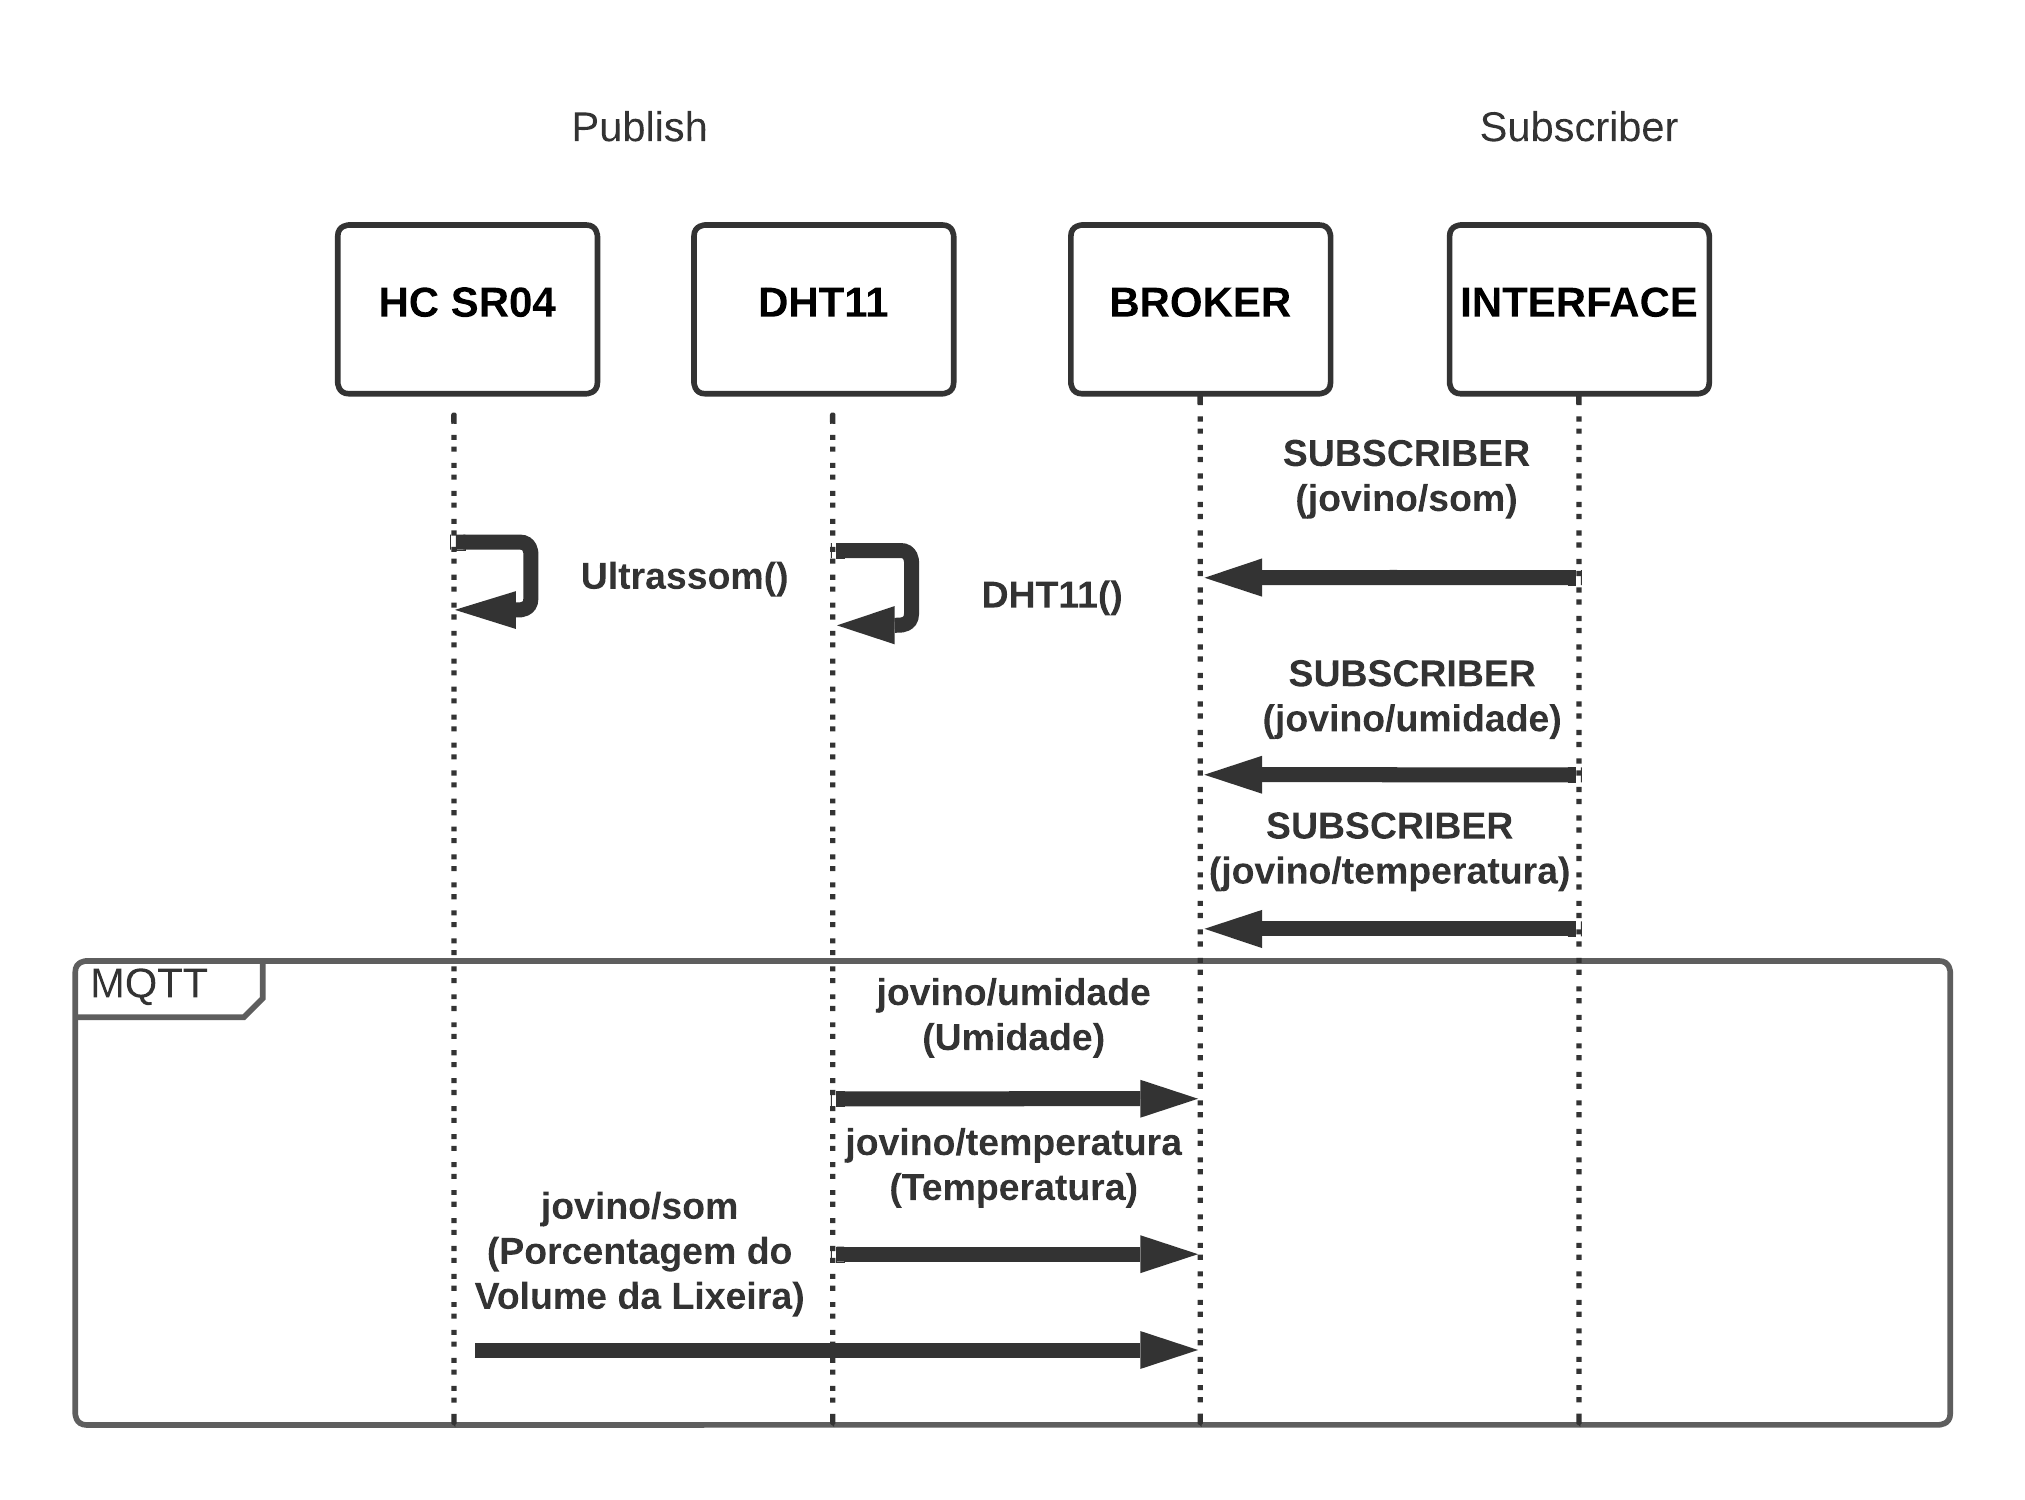
\includegraphics[width=\linewidth]{figures/mqtt.png}
    \caption{Sequência de publicação/assinatura (2024)}
  \end{subfigure}\hfill
  \begin{subfigure}{0.30\textwidth}\centering
    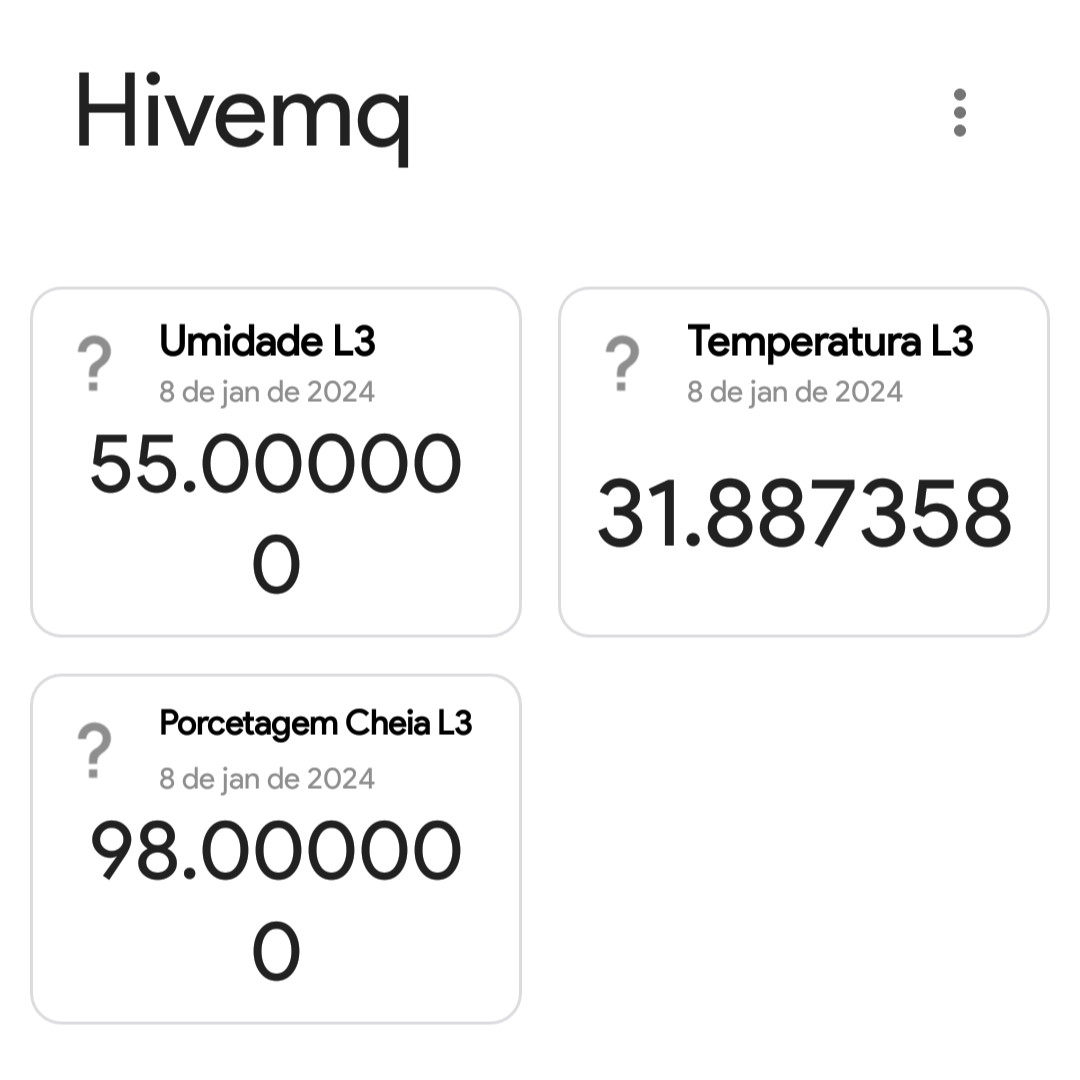
\includegraphics[width=\linewidth]{figures/dashboard.jpg}
    \caption{Aplicativo MQTT Dashboard}
  \end{subfigure}
  \caption{Material do protótipo de 2024, reproduzido do trabalho original.}
  \label{fig:prototipo}
\end{figure}

A auditoria do código original identificou 27 defeitos, cada um verificado no
código e, quando aplicável, na documentação das bibliotecas e nas folhas de
dados. A Tabela~\ref{tab:auditoria} resume os de maior impacto. Dois deles
comprometem diretamente a medida usada no trabalho: a ``porcentagem de volume''
era calculada como $d/T_{\max}\cdot 100$, que \emph{cresce} quando a lixeira
esvazia, e, em caso de eco perdido, a biblioteca de ultrassom usada retornava
51~cm, valor que a fórmula convertia em 102\%. O código também continha
credenciais de Wi-Fi em texto claro, publicadas em repositório público; elas
não são reproduzidas aqui, e recomenda-se trocá-las.

\begin{table}[ht]
\centering
\caption{Principais defeitos do firmware de 2024 e correções (auditoria completa em \texttt{firmware/AUDITORIA.md}).}
\label{tab:auditoria}
\footnotesize
\begin{tabularx}{\textwidth}{@{}>{\raggedright\arraybackslash}p{4.6cm}>{\raggedright\arraybackslash}X@{}}
\toprule
Defeito & Correção no firmware 2.0 \\
\midrule
Percentual proporcional ao espaço vazio, sem limites & ocupação $=100(H-(d-\mathit{off}))/H$, limitada a $[0,100]$ \\
Eco perdido convertido em 51~cm (102\%) & \texttt{pulseIn} com tempo limite; mediana de 5 pulsos com quórum de 3; \texttt{valida=false} \\
Índice de calor publicado como ``temperatura'' & publica a temperatura do ar \\
\texttt{dht.begin()} ausente; LED como entrada & inicialização corrigida \\
Broker público, sem autenticação nem TLS & broker configurável, usuário/senha, TLS opcional \\
Laços bloqueantes de Wi-Fi e MQTT & máquina de estados não bloqueante, recuo exponencial com \emph{jitter} \\
Sem LWT, sem estado, sem sequência & LWT retido, estado \texttt{online}, \texttt{boot} em NVS e \texttt{seq} \\
ECHO (5~V) direto em GPIO de 3,3~V & divisor 1~k$\Omega$/2~k$\Omega$ ($\approx 3{,}33$~V) \\
ECHO no GPIO12 (pino de \emph{strapping} da tensão da flash) & ECHO movido para o GPIO27 \\
Credenciais no código & \texttt{config.h} fora do controle de versão \\
\bottomrule
\end{tabularx}
\end{table}

O firmware 2.0 separa medição, transmissão e rede em módulos e usa um
agendador baseado em \texttt{millis()}, sem \texttt{delay()} no laço principal.
A distância é a mediana de uma rajada de cinco pulsos espaçados em 65~ms (a
folha de dados recomenda ciclo superior a 60~ms \cite{elecfreakssdhcsr04}),
com compensação opcional da velocidade do som pela temperatura do DHT11. A
telemetria é publicada a cada 60~s por padrão, com intervalo ajustável por
comando remoto. Eventos de limiar usam histerese, e um \emph{watchdog} de 30~s
reinicia o dispositivo em caso de travamento.

O firmware foi compilado com o \texttt{arduino-cli} 1.5.1 e o núcleo
\texttt{esp32} 3.3.12 para a placa DOIT ESP32 DevKit~V1, com todos os avisos
habilitados, sem erros nem avisos. A variante padrão ocupa \num{941910} bytes
de flash (71\%) e \num{51284} bytes de RAM estática (15\%). O firmware
\emph{não} foi executado em placa real nem no simulador Wokwi: o protótipo
físico não estava disponível, e a execução automatizada do Wokwi exige uma
credencial que não foi criada. Os arquivos de circuito para o Wokwi estão no
repositório, prontos para uso, mas não constituem resultado deste trabalho.
Assim, o comportamento em tempo de execução do firmware 2.0 permanece não
verificado; o que é verificado em execução é o contrato MQTT, exercitado pelos
dispositivos virtuais.

\subsection{Contrato de mensagens MQTT}

Os tópicos seguem o padrão \texttt{residuos/dispositivos/\{id\}/\{tipo\}}, com
quatro tipos (Tabela~\ref{tab:topicos}). A plataforma assina
\texttt{residuos/dispositivos/+/telemetria}, \texttt{.../+/estado} e
\texttt{.../+/eventos}. A Figura~\ref{fig:mqtt_seq} ilustra a sequência de
conexão, publicação e queda abrupta.

\begin{table}[ht]
\centering
\caption{Tópicos do contrato MQTT (esquema versão 1).}
\label{tab:topicos}
\footnotesize
\begin{tabular}{@{}llccl@{}}
\toprule
Sufixo & Sentido & QoS & Retido & Conteúdo \\
\midrule
\texttt{telemetria} & dispositivo $\to$ plataforma & 0 (ESP32) / 1 (virtual) & não & leituras periódicas \\
\texttt{estado} & dispositivo $\to$ plataforma & 1 & sim & \texttt{online}/\texttt{offline}; LWT \\
\texttt{eventos} & dispositivo $\to$ plataforma & 0/1 & não & limiar, falha de sensor, reinício \\
\texttt{comandos} & plataforma $\to$ dispositivo & 1 & não & intervalo, LED, \emph{ping} \\
\bottomrule
\end{tabular}
\end{table}

\begin{figure}[ht]
  \centering
  \resizebox{\textwidth}{!}{% Sequência MQTT: conexão com LWT, telemetria, falha abrupta
\begin{tikzpicture}[font=\sffamily\tiny, >={Stealth[length=1.7mm]}]
\def\yb{-8.6}
\foreach \x/\n/\c in {0/Dispositivo (ESP32 ou virtual)/orange!12, 6.4/Broker Mosquitto/blue!10, 12.8/Plataforma (ingestão)/green!10}{
  \node[draw, rounded corners=2pt, fill=\c, minimum width=30mm, minimum height=6mm] at (\x,0) {\n};
  \draw[dashed, gray] (\x,-0.3) -- (\x,\yb);}
\draw[->] (12.8,-0.8) -- node[above]{SUBSCRIBE \texttt{.../+/telemetria|estado|eventos} (QoS 1)} (6.4,-0.8);
\draw[->] (0,-1.5) -- node[above, align=center]{CONNECT (id = \texttt{LX-0007}, keepalive 15 s)\\Will: \texttt{.../estado} = offline, QoS 1, retido} (6.4,-1.5);
\draw[->] (0,-2.3) -- node[above]{PUBLISH \texttt{.../estado} = online (retido)} (6.4,-2.3);
\draw[->] (6.4,-2.6) -- (12.8,-2.6);
\foreach \y in {-3.4,-4.1}{
  \draw[->] (0,\y) -- node[above]{PUBLISH \texttt{.../telemetria} \{v, id, boot, seq, ts, leituras\}} (6.4,\y);
  \draw[->] (6.4,\y-0.2) -- (12.8,\y-0.2);}
\node[anchor=west, align=left] at (12.9,-3.9) {valida esquema\\deduplica (id, boot, seq)\\filtro de mediana};
\draw[->] (0,-5.0) -- node[above]{PUBLISH \texttt{.../eventos} \{tipo: limiar\_excedido\}} (6.4,-5.0);
\draw[->] (6.4,-5.2) -- (12.8,-5.2);
\node[red!70!black, font=\sffamily\scriptsize\bfseries] at (0,-6.0) {$\times$ queda sem DISCONNECT};
\draw[->, red!70!black] (6.4,-6.6) -- node[above]{Will: \texttt{.../estado} = offline, motivo = lwt (retido)} (12.8,-6.6);
\draw[->] (0,-7.6) -- node[above]{reconexão com recuo exponencial (1 $\to$ 32 s); estado = online} (6.4,-7.6);
\end{tikzpicture}
}
  \caption{Sequência de mensagens do contrato: conexão com \emph{Last Will}, publicação de estado retido, telemetria, evento e publicação do LWT pelo broker após queda sem DISCONNECT.}
  \label{fig:mqtt_seq}
\end{figure}

Cada telemetria é um objeto JSON com versão do esquema (\texttt{v}),
identificador (\texttt{id}), contador de inicializações persistido em memória
não volátil (\texttt{boot}), número de sequência (\texttt{seq}), instante da
medição (\texttt{ts}), origem do relógio (\texttt{ts\_src}) e uma lista de
leituras, cada uma com tipo, valor, unidade e validade:

\begin{small}
\begin{verbatim}
{"v":1, "id":"LX-0007", "boot":4, "seq":1532, "ts":1731580000, "ts_src":"ntp",
 "leituras":[{"tipo":"distancia","valor":31.2,"unidade":"cm","valida":true},
             {"tipo":"ocupacao","valor":78.8,"unidade":"%","valida":true}]}
\end{verbatim}
\end{small}

O par (\texttt{boot}, \texttt{seq}) identifica unicamente cada mensagem de um
dispositivo, o que permite descartar duplicatas geradas por reentregas com
QoS~1 sem confundi-las com mensagens novas após reinicialização.

\subsection{Ingestão e estado estimado}

A ingestão aplica, nesta ordem: validação de esquema (versão, coerência entre
\texttt{id} e tópico, tipos, unidades e faixa da ocupação); deduplicação por
(\texttt{id}, \texttt{boot}, \texttt{seq}); registro do último contato; descarte
de leituras inválidas para fins de estado; e rejeição, para o estado corrente,
de mensagens com instante anterior ao último estado aplicado ou à última coleta
registrada. A ocupação observada $\hat f_i$ é a mediana das três últimas
leituras válidas do ciclo corrente, o que elimina leituras espúrias isoladas.
Como a mediana introduz um atraso de uma leitura quando há tendência, o
instante associado ao estado é o da leitura mediana, e não o da mais recente;
esse detalhe foi revelado por um teste automatizado.

A taxa de enchimento $\hat r_i$ (fração do volume por hora) é estimada por
mínimos quadrados sobre as leituras das últimas 48~h do ciclo corrente, desde
que haja ao menos 6 leituras cobrindo 12~h; na falta delas, usa-se uma média
móvel exponencial ($\alpha = 0{,}3$) das taxas de ciclos anteriores e, por
último, a mediana das taxas da frota. A projeção para um instante futuro é
$\tilde f_i(t) = \hat f_i + \hat r_i\,(t - t^{\mathrm{obs}}_i)$. Um contêiner
cujo último estado tem mais de 24~h é marcado como \emph{desatualizado}; nesse
caso, as políticas podem usar a estimativa por taxa de longo prazo
(\emph{fallback}) ou manter o último valor observado. Quando um veículo
registra uma coleta, o estado é zerado e um novo ciclo começa.

\subsection{Persistência}

O SQLite armazena todas as mensagens de telemetria recebidas, com o resultado
da ingestão (aplicada, duplicada, fora de ordem ou inválida), o estado de
disponibilidade de cada dispositivo, os eventos, as mensagens rejeitadas, as
rotas planejadas e as coletas executadas. Nos experimentos em lote, os
resultados são gravados em arquivos JSON Lines, uma linha por execução, com a
configuração completa, a semente e as métricas; um manifesto registra o
\emph{commit} do código, as versões das dependências e a plataforma.

\subsection{Simulador}

O simulador é de tempo discreto, com passo de 15~min
(Figura~\ref{fig:simulacao}). Antes da execução, são sorteados, a partir de
fluxos aleatórios independentes derivados da semente, a geometria do cenário,
a matriz de geração de resíduos, os ruídos e falhas dos sensores e as perdas e
atrasos do canal. Como esses sorteios não dependem da política, duas políticas
executadas com a mesma semente enfrentam exatamente as mesmas condições, o que
foi verificado por teste automatizado.

\begin{figure}[ht]
  \centering
  % Laço da simulação em tempo discreto
\begin{tikzpicture}[font=\sffamily\scriptsize, node distance=3.2mm,
  st/.style={draw, rounded corners=2pt, text width=58mm, align=left, inner sep=3pt, fill=#1},
  st/.default=white, arr/.style={-{Stealth[length=1.8mm]}, thick}]
\node[st=gray!10] (init) {\textbf{Inicialização} (semente $s$): malha e posições; matriz de geração $q_{i,t}$; fluxos de ruído, falhas e perdas (números aleatórios comuns a todas as políticas)};
\node[st=red!8, below=of init] (plan) {\textbf{Se $t$ = 06h:} política escolhe contêineres e o OR-Tools gera as rotas do dia a partir do \emph{estado estimado}};
\node[st=orange!10, below=of plan] (gen) {\textbf{Geração:} $f_i \leftarrow f_i + q_{i,t}/V$; excedente acima de $V$ = transbordamento};
\node[st=yellow!15, below=of gen] (truck) {\textbf{Veículos:} avançam até o fim do passo; coletam o volume \emph{verdadeiro}; desvio ao depósito se a carga exceder $Q$; retornam se a jornada não comportar a próxima visita};
\node[st=blue!8, below=of truck] (sense) {\textbf{Sensores:} dispositivos programados medem $d$ (ruído, viés de superfície, falhas) e transmitem pelo canal (perda, atraso, duplicação, interrupções)};
\node[st=green!10, below=of sense] (ing) {\textbf{Ingestão:} mensagens que chegam no passo são validadas, deduplicadas e filtradas; atualiza ocupação e taxa estimadas};
\node[st=purple!8, below=of ing] (met) {\textbf{Métricas} (somente após 7 dias de aquecimento): km, visitas, transbordamento, ocupação na coleta, espera, telemetria, balanço de volume};
\draw[arr] (init) -- (plan);
\foreach \a/\b in {plan/gen, gen/truck, truck/sense, sense/ing, ing/met} \draw[arr] (\a) -- (\b);
\draw[arr] (met.east) -- ++(5mm,0) |- node[pos=0.25, right, align=left] {$t \leftarrow t+1$\\(15 min)} (plan.east);
\end{tikzpicture}

  \caption{Laço da simulação. As decisões usam apenas o estado estimado; o
  estado verdadeiro é usado na geração, na execução das coletas e nas
  métricas.}
  \label{fig:simulacao}
\end{figure}

A separação entre estado verdadeiro e estado estimado é central. As políticas
B, C e D só enxergam o que chegou pela telemetria; o estado verdadeiro é usado
para gerar resíduos, para determinar o volume efetivamente recolhido na
chegada do veículo e para calcular as métricas. A cada execução, o simulador
verifica o balanço de volume na janela avaliada: o volume gerado deve ser igual
à soma do volume coletado, do volume transbordado e da variação do estoque nos
contêineres.

O modo \emph{live} usa as mesmas classes, mas substitui o canal emulado pelo
broker: cada contêiner virtual é um cliente MQTT próprio, com LWT e
reconexão automática (paho-mqtt 2.2, MQTT 3.1.1), e a plataforma é um
assinante com sessão persistente que alimenta a mesma rotina de ingestão.
Nos experimentos em lote, o canal emulado permite processar centenas de
milhares de mensagens por execução; a equivalência entre os dois caminhos é
verificada no experimento E6.

\subsection{Políticas de coleta e roteirização}\label{sec:politicas}

A Figura~\ref{fig:planejamento} resume a decisão diária, tomada às 06h para o
turno das 07h às 15h. As quatro políticas diferem apenas na seleção dos
contêineres e na forma de atribuir prêmios; frota, capacidade, jornada,
velocidade, tempos de atendimento e regra de execução são os mesmos.

\begin{figure}[ht]
  \centering
  \resizebox{0.95\textwidth}{!}{% Fluxo de decisão diária e execução
\begin{tikzpicture}[font=\sffamily\scriptsize,
  b/.style={draw, rounded corners=2pt, align=center, minimum height=9mm, fill=#1},
  b/.default=white, d/.style={draw, diamond, aspect=2.2, align=center, inner sep=1pt, fill=yellow!12},
  arr/.style={-{Stealth[length=1.8mm]}, thick}]
\node[b=green!10, text width=34mm] (est) at (0,0) {Estado estimado\\$\hat f_i$, $\hat r_i$, idade do dado};
\node[d] (stale) at (0,-1.45) {dado\\$>$ 24 h?};
\node[b, text width=30mm] (fb) at (3.6,-1.45) {\emph{fallback}:\\$\hat f_i + \hat r^{\,\mathrm{longo}}_i\,\Delta t$};
\node[d] (pol) at (0,-3.0) {política};
\node[b=red!6, text width=24mm] (A) at (-4.95,-4.6) {\textbf{A}: vencidos no calendário $p_i$ e pendentes};
\node[b=red!6, text width=20mm] (B) at (-1.95,-4.6) {\textbf{B}: $\hat f_i \ge \theta_{hi}$\\(todos obrigatórios)};
\node[b=red!6, text width=24mm] (C) at (1.0,-4.6) {\textbf{C}: obrig. $\hat f_i\ge\theta_{hi}$\\opc. $\hat f_i\ge\theta_{lo}$};
\node[b=red!6, text width=29mm] (D) at (4.45,-4.6) {\textbf{D}: obrig. se $\tilde f_i(t_{\text{meio}})\ge\theta_{hi}$\\ou $\tilde f_i(t_{\text{próx}})\ge\theta_{crit}$};
\node[b=blue!8, text width=96mm] (vrp) at (0,-6.55) {CVRP com prêmios: $\min \sum d_{ij} + \sum_{i\ \text{não visitado}} \pi_i$ \quad (capacidade $Q$, jornada $T_{\max}$, $K$ veículos)\\OR-Tools com descida gulosa (A, B-OR, C, D) ou vizinho mais próximo + 2-opt (B)};
\node[b=yellow!15, text width=96mm] (exe) at (0,-8.25) {Execução com volumes verdadeiros: desvio ao depósito se a carga exceder $Q$;\\visitas que não cabem na jornada ficam não realizadas (A as reprograma para o dia seguinte)};
\draw[arr] (est) -- (stale);
\draw[arr] (stale) -- node[above]{sim} (fb);
\draw[arr] (fb) |- (pol);
\draw[arr] (stale) -- node[left]{não} (pol);
\foreach \x in {A,B,C,D} \draw[arr] (pol) -- (\x.north);
\foreach \x in {A,B,C,D} \draw[arr] (\x.south) -- (\x.south |- vrp.north);
\draw[arr] (vrp) -- (exe);
\end{tikzpicture}
}
  \caption{Decisão diária de coleta e execução das rotas.}
  \label{fig:planejamento}
\end{figure}

\begin{description}
  \item[A -- periódica fixa.] Cada contêiner recebe um período
  $p_i = \min(7, \max(1, \lfloor \gamma V/\mu_i \rfloor))$ dias, em que
  $\mu_i$ é a taxa média de geração de longo prazo e $\gamma = 0{,}8$ é a
  ocupação média desejada na coleta; as fases são distribuídas para equilibrar
  a carga diária. A política usa a taxa média \emph{verdadeira} do simulador,
  o que equivale a um planejador com histórico perfeito. Trata-se de uma
  linha de base deliberadamente exigente: a coleta fixa não é penalizada por
  um mau dimensionamento de frequências. Visitas não realizadas são
  reprogramadas para o dia seguinte.
  \item[B -- limiar.] São obrigatórios os contêineres com $\hat f_i \ge
  \theta_{hi} = 0{,}75$. As rotas são construídas pelo vizinho mais próximo,
  respeitando capacidade e jornada, e melhoradas por 2-opt. A variante B-OR
  usa a mesma seleção com o OR-Tools, para separar o efeito da seleção do
  efeito do roteirizador.
  \item[C -- dinâmica otimizada.] São obrigatórios os contêineres com
  $\hat f_i \ge \theta_{hi}$ e opcionais os com $\theta_{lo} = 0{,}50 \le
  \hat f_i < \theta_{hi}$. O prêmio de um opcional é $\pi_i = \lambda\,\hat
  f_i V$, com $\lambda = 1$~m por litro: o contêiner entra na rota se o desvio
  necessário for menor que o prêmio.
  \item[D -- preditiva.] Como C, mas com ocupações projetadas pela taxa
  estimada. É obrigatório o contêiner cuja projeção para o meio do turno é
  $\ge \theta_{hi}$ ou cuja projeção para o fim do turno seguinte é $\ge
  \theta_{crit} = 0{,}95$, isto é, que provavelmente transbordaria antes da
  próxima oportunidade de coleta.
\end{description}

O problema diário é um CVRP com prêmios. Sejam $S$ o conjunto de contêineres
selecionados, $K$ o número de veículos, $Q$ a capacidade por viagem, $q_i$ o
volume estimado, $d_{ij}$ a distância na malha (assimétrica, por causa das vias
de sentido único), $t_{ij}$ o tempo de viagem, $s$ o tempo de atendimento e
$T_{\max}$ a jornada. O resolvedor busca rotas $R_1,\dots,R_K$ que minimizem
\begin{equation}
  \sum_{k=1}^{K}\sum_{(i,j)\in R_k} d_{ij} \;+\; \sum_{i\in S\setminus \cup_k R_k} \pi_i
  \label{eq:objetivo}
\end{equation}
sujeitas a $\sum_{i\in R_k} q_i \le Q$ e $\sum_{(i,j)\in R_k}(t_{ij}+s) \le
T_{\max}$ para todo $k$. Contêineres obrigatórios recebem $\pi_i = 10^8$,
valor superior a qualquer distância possível, de modo que só são omitidos
quando não há solução viável que os inclua. O OR-Tools 9.15 é configurado com
solução inicial pelo arco mais barato e busca local por descida gulosa até um
ótimo local. Essa configuração é determinística: a mesma entrada produz sempre
a mesma rota, independentemente da velocidade da máquina. O efeito de
substituí-la pela busca local guiada, interrompida por tempo, é medido no
experimento E5.

Na execução, o veículo chega a cada contêiner e recolhe o volume verdadeiro
naquele instante. Se a carga excederia $Q$, ele vai ao depósito, descarrega e
retorna \cite{dror1989vehicle}; se a jornada não comporta a próxima visita e o
retorno, ele encerra a rota, e as visitas restantes são registradas como não
realizadas.

\subsection{Painel operacional}\label{sec:painel}

O painel web foi construído com FastAPI no servidor e HTML, CSS e JavaScript
sem bibliotecas externas no navegador, para funcionar sem acesso à internet.
Ele lê exclusivamente dados produzidos pela aplicação: o estado escrito pelo
modo \emph{live} a cada passo, o banco SQLite alimentado pela ingestão MQTT,
um traço gravado de simulação e o resumo dos experimentos. Há três visões:

\begin{itemize}
  \item \textbf{Operação ao vivo} (Figura~\ref{fig:painel}a): mapa da malha
  viária com os contêineres coloridos pela ocupação estimada, contêineres sem
  dado recente em contorno, dispositivos \emph{offline} marcados, depósito,
  veículos e rotas do dia desenhadas pelas ruas; indicadores de distância,
  coletas, transbordamento, dispositivos \emph{online} e mensagens
  (recebidas, duplicadas e rejeitadas); filtros por estado; histórico de
  telemetria de cada contêiner, consultado no SQLite; e lista de eventos
  MQTT. Um seletor alterna entre o estado estimado pela plataforma e o estado
  verdadeiro do simulador, o que permite observar a diferença entre o que o
  operador vê e o que de fato ocorre.
  \item \textbf{\emph{Replay} A $\times$ D} (Figura~\ref{fig:painel}b):
  reprodução sincronizada de duas execuções com a mesma semente, com controle
  de tempo e velocidade.
  \item \textbf{Resultados}: tabela do experimento E1 e fronteira do E2, lidas
  do resumo gerado pela análise.
\end{itemize}

\begin{figure}[ht]
  \centering
  \begin{subfigure}{\textwidth}\centering
    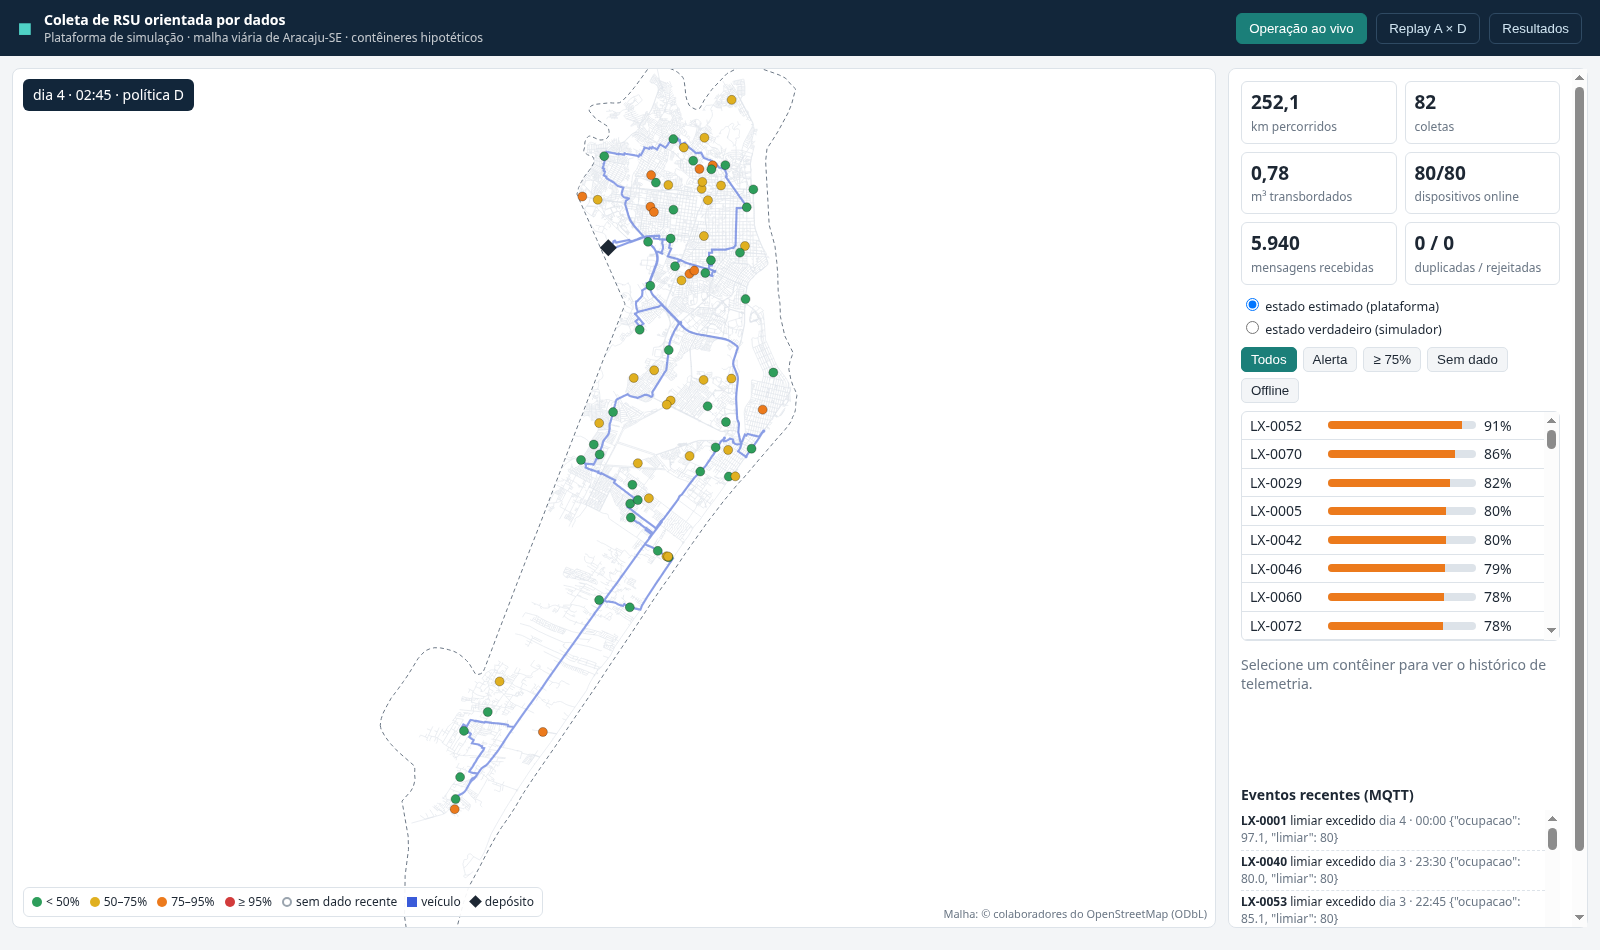
\includegraphics[width=0.93\textwidth]{figures/painel_ao_vivo.png}
    \caption{Operação ao vivo: telemetria recebida pelo broker, rotas do dia e histórico de um contêiner.}
  \end{subfigure}\\[4pt]
  \begin{subfigure}{\textwidth}\centering
    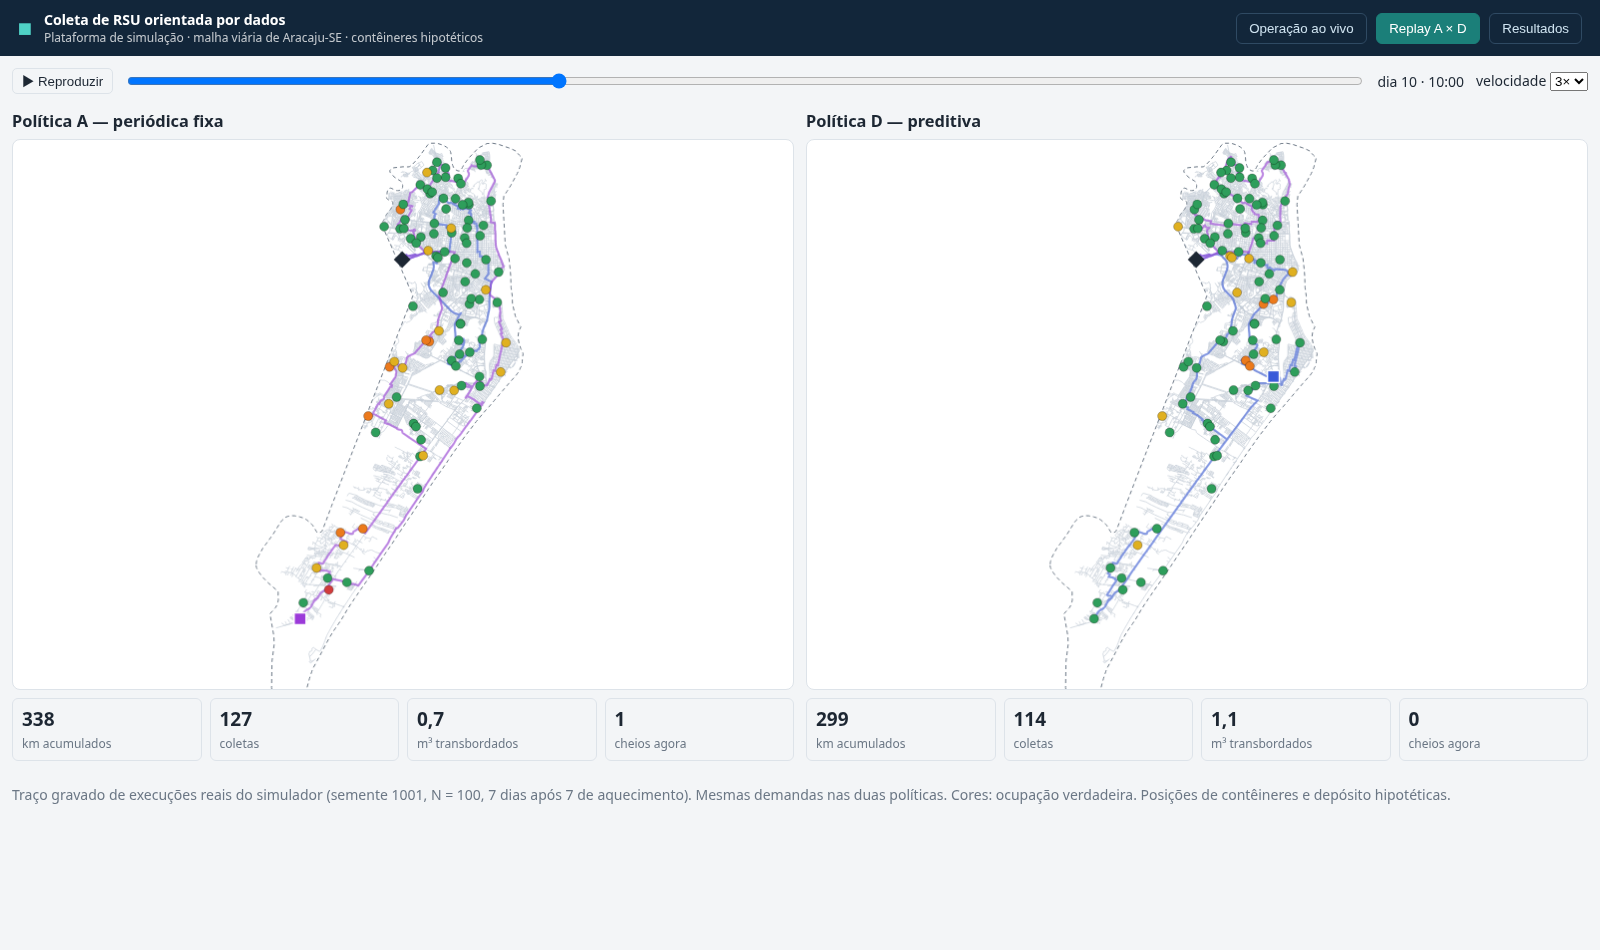
\includegraphics[width=0.93\textwidth]{figures/painel_replay.png}
    \caption{Replay sincronizado das políticas A e D (semente 1001, $N = 100$).}
  \end{subfigure}
  \caption{Capturas do painel operacional, obtidas com a aplicação em execução (navegador em modo \emph{headless}).}
  \label{fig:painel}
\end{figure}


\subsection{Verificação do software}

O pacote tem \NTestes{} testes automatizados (pytest), que cobrem: a fórmula de
ocupação e seus limites físicos; leituras inválidas; o viés de superfície do
modelo de sensor, comparado ao valor teórico $\sigma\sqrt{2/\pi}$; a fração de
indisponibilidade do processo de falhas, comparada a
$\mathrm{MTTR}/(\mathrm{MTBF}+\mathrm{MTTR})$; a média de longo prazo da
geração; o determinismo por semente; a validação do esquema de mensagens; a
deduplicação, a ordenação e o filtro de mediana; a estimativa de taxa em uma
série linear; o roteirizador em instâncias pequenas, comparado à enumeração
exata; o respeito à capacidade e à jornada; o balanço de volume para as quatro
políticas; e o uso de números aleatórios comuns entre políticas.

\section{Metodologia experimental}\label{sec:metodologia}

\subsection{Caracterização da pesquisa}

Trata-se de uma pesquisa aplicada, de abordagem quantitativa, conduzida por
experimentos computacionais com um modelo de simulação estocástica. O
protocolo (hipóteses, sementes, métricas e testes) foi registrado no
repositório antes das rodadas definitivas (\texttt{docs/protocolo-experimental.md}).
As rodadas-piloto, usadas para depuração e para medir o custo computacional,
empregaram as sementes 1 e 3; as rodadas definitivas usam as sementes 1001 a
1030, e os resultados do piloto não entram em nenhuma análise.

\subsection{Modelos}

\paragraph{Geração de resíduos.}
Para o contêiner $i$, no passo $t$ do dia $d$ (dia da semana $w$, hora $h$), o
volume solto gerado, em litros, é
\begin{equation}
  q_{i,t} = \mu_i \, I \, W_{p_i}(w) \, Z_{i,d} \, H_{p_i}(h) \, E_{i,t} + e_{i,t},
  \label{eq:demanda}
\end{equation}
em que $\mu_i$ é a taxa média diária de longo prazo, $I$ é a intensidade do
cenário, $W_p$ e $H_p$ são os perfis semanal (média 1) e horário (soma 1) do
perfil $p_i \in \{$residencial, comercial, institucional$\}$, $Z_{i,d}$ e
$E_{i,t}$ são fatores Gama de média 1 que representam a variação entre dias
(CV 0,25) e a chegada irregular dos descartes ao longo do dia (CV 1,0), e
$e_{i,t}$ representa descartes volumosos esporádicos (processo de Poisson, em
média um a cada 30 dias por contêiner, com 15\% a 45\% do volume do
contêiner). A heterogeneidade entre contêineres é dada por
$\mu_i = \bar\mu_{p_i}\,\eta_i$, com $\eta_i$ lognormal de média 1 e CV 0,35.
A distribuição Gama foi escolhida por ser não negativa e permitir controlar a
média e o coeficiente de variação de forma independente; a lognormal, por
produzir a assimetria à direita esperada entre pontos de coleta.

\paragraph{Estado do contêiner e transbordamento.}
A ocupação verdadeira $f_i \in [0,1]$ evolui como $f_i \leftarrow f_i +
q_{i,t}/V$. Se o resultado excede 1, o excedente $(f_i-1)V$ é contabilizado
como volume transbordado e $f_i$ é limitado a 1. O modelo, portanto, não
supõe que o resíduo excedente seja recolhido depois; ele representa uma falha
de serviço. Uma coleta zera $f_i$.

\paragraph{Sensor ultrassônico.}
Com contêiner prismático de seção constante, a fração de volume é igual à
fração de altura (Figura~\ref{fig:conteiner}). Com $D_0$ a distância do sensor
ao fundo, $\mathit{off}$ a zona morta de montagem e $H = D_0 - \mathit{off}$,
a distância verdadeira até a superfície é $d = D_0 - f H$, e a ocupação
calculada pelo firmware e pela plataforma é
\begin{equation}
  \hat o(d) = 100 \cdot \min\!\left\{1, \max\!\left\{0, \frac{H - (d - \mathit{off})}{H}\right\}\right\},
  \label{eq:ocupacao}
\end{equation}
considerada inválida se $d$ estiver fora de $[2, 400]$~cm ou além do fundo
($d > D_0 + 15$~cm). A medição simulada é
\begin{equation}
  d^{\mathrm{med}} = d + \sigma_r\,\varepsilon_1 - \sigma_s\,|\varepsilon_2|,\qquad
  \varepsilon_1,\varepsilon_2 \sim \mathcal N(0,1),
  \label{eq:sensor}
\end{equation}
em que o termo semi-normal negativo representa o retorno do primeiro eco pelo
ponto mais alto de uma superfície irregular e produz um viés de
superestimação da ocupação de $\sigma_s\sqrt{2/\pi}$. Com probabilidade de 1\%
a leitura é perdida (sem eco) e com 0,5\% é espúria, entre 3 e 20~cm,
simulando uma obstrução momentânea. A
Figura~\ref{fig:sensor}(b) mostra 1.500 leituras simuladas nos níveis base e
de ruído seis vezes maior. A formulação não se aplica a geometrias não
prismáticas sem uma curva altura--volume específica.

\begin{figure}[ht]
  \centering
  % Modelo geométrico do contêiner instrumentado
\begin{tikzpicture}[font=\sffamily\scriptsize, >={Stealth[length=1.6mm]}]
\def\W{3.2}\def\Hb{4.4}\def\off{0.4}\def\fl{1.9}
\fill[brown!35] (0,0) -- (\W,0) -- (\W,\fl) .. controls (2.2,\fl+0.35) and (1.2,\fl-0.25) .. (0,\fl+0.1) -- cycle;
\draw[thick] (0,\Hb) -- (0,0) -- (\W,0) -- (\W,\Hb);
\draw[thick] (-0.15,\Hb) -- (\W+0.15,\Hb);
\node[draw, fill=blue!15, minimum width=10mm, minimum height=3mm, inner sep=0] (s) at (\W/2,\Hb-0.15) {};
\node[above=1mm of s] {HC-SR04};
\fill[blue!8, opacity=.6] (\W/2-0.08,\Hb-0.3) -- (\W/2-0.08-0.55,1.95) -- (\W/2+0.08+0.55,2.05) -- (\W/2+0.08,\Hb-0.3) -- cycle;
\node[blue!60!black] at (\W/2+0.95,3.0) {cone $\approx 15^\circ$};
\draw[dashed, gray] (0,\Hb-\off) -- (\W,\Hb-\off);
\draw[<->] (\W+0.5,0) -- node[right] {$D_0$} (\W+0.5,\Hb-0.3);
\draw[<->] (\W+1.2,\Hb-0.3) -- node[right] {$\mathit{off}$} (\W+1.2,\Hb-\off);
\draw[<->] (\W+1.2,0) -- node[right] {$H = D_0-\mathit{off}$} (\W+1.2,\Hb-\off);
\draw[<->, red!70!black] (\W/2+0.15,\Hb-0.3) -- node[right] {$d$} (\W/2+0.15,2.08);
\draw[<->] (-0.4,0) -- node[left, align=right] {altura\\ocupada\\$h$} (-0.4,\fl);
\node[align=center] at (\W/2,0.7) {resíduos\\(superfície irregular)};
\end{tikzpicture}

  \caption{Geometria adotada para o contêiner instrumentado.}
  \label{fig:conteiner}
\end{figure}

\begin{figure}[ht]
  \centering
  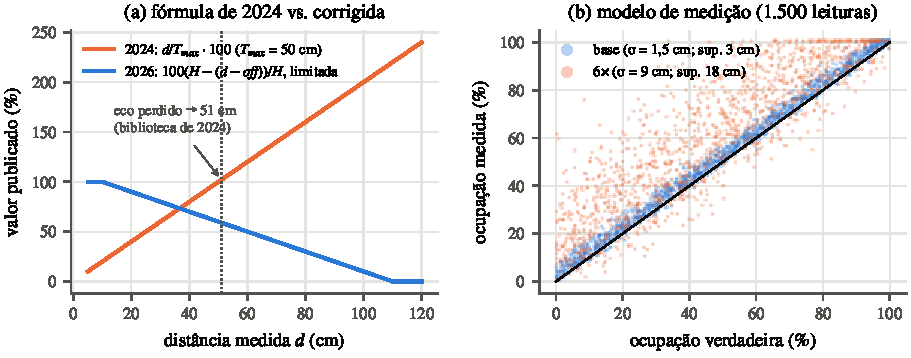
\includegraphics[width=\textwidth]{figures/fig_sensor.pdf}
  \caption{(a) Valor publicado em função da distância medida: a fórmula de 2024
  cresce quando o contêiner esvazia e ultrapassa 100\%; a fórmula corrigida
  é limitada a $[0,100]$. (b) Ocupação medida $\times$ verdadeira pelo modelo
  de sensor (Equação~\ref{eq:sensor}), nos níveis de ruído base e 6$\times$.}
  \label{fig:sensor}
\end{figure}

\paragraph{Disponibilidade e canal.}
Cada dispositivo alterna entre operacional e indisponível segundo uma cadeia
de Markov de dois estados, com tempo médio entre falhas de 60 dias e tempo
médio de reparo de 12~h. Opcionalmente, uma fração dos dispositivos falha
definitivamente em instante uniforme no horizonte, ou passa a repetir a mesma
leitura (sensor ``congelado''). Cada mensagem é perdida com probabilidade
$p_{\mathrm{perda}}$, duplicada com probabilidade 0,2\% e atrasada segundo uma
lognormal de mediana 0,5~s, com 0,2\% de atrasos longos (1 a 6~h). Interrupções
regionais tornam inacessíveis os dispositivos mais próximos de um centro
sorteado durante um intervalo; o firmware não armazena leituras para reenvio,
de modo que as mensagens desse período são perdidas.

\paragraph{Planejamento e execução.}
As políticas e a formulação do CVRP com prêmios foram apresentadas na
Seção~\ref{sec:politicas} (Equação~\ref{eq:objetivo}).

\subsection{Cenário, dados e parâmetros}\label{sec:parametros}

O cenário usa a malha viária dirigível do município de Aracaju, extraída do
OpenStreetMap \cite{haklay2008openstreetmap} a partir do extrato da região
Nordeste distribuído pela Geofabrik \cite{geofabrik2026nordeste}, com
integridade conferida por MD5. O limite municipal é a relação administrativa
do próprio OSM. Mantiveram-se as vias de uso automotivo, os sentidos de
circulação e a maior componente fortemente conexa: \num{45011} nós,
\num{86410} arcos dirigidos e \num{3058,7}~km de arcos. Os contêineres são
posicionados em interseções sorteadas (uniformemente, ou em agrupamentos no
experimento E4), o que faz a densidade de contêineres acompanhar a densidade
de ruas. O depósito é o nó mais próximo de um ponto hipotético no oeste da
área urbana (Figura~\ref{fig:cenario}). As distâncias são caminhos mínimos na
malha dirigida, calculados pelo algoritmo de Dijkstra (SciPy
\cite{virtanen2020scipy}).

\begin{figure}[ht]
  \centering
  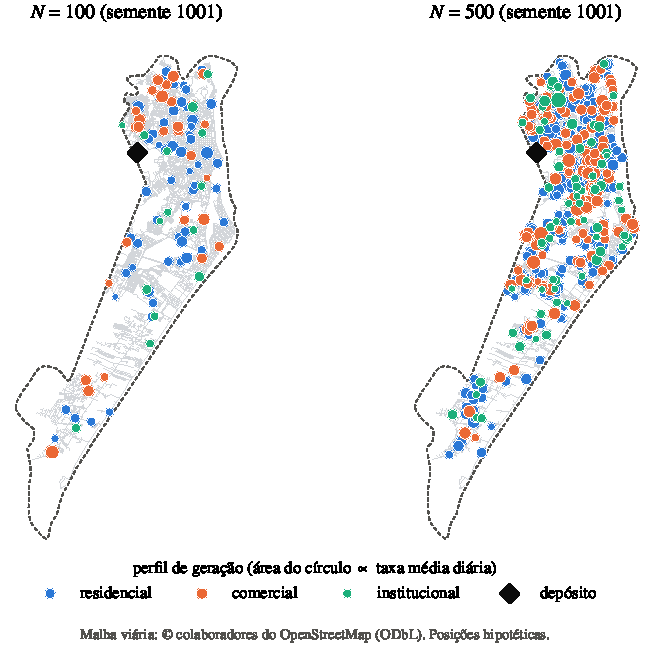
\includegraphics[width=0.92\textwidth]{figures/fig_cenario.pdf}
  \caption{Contêineres simulados sobre a malha viária de Aracaju para 100 e 500
  contêineres (semente 1001). As posições e o depósito são hipotéticos e não
  correspondem a equipamentos existentes.}
  \label{fig:cenario}
\end{figure}

A Tabela~\ref{tab:parametros} separa os parâmetros segundo sua natureza: dado
público observado (P), dado geográfico real (G), valor da literatura (L),
hipótese de cenário (H) e dado sintético (S). Os parâmetros de demanda são
hipóteses ancoradas em dados oficiais: com geração domiciliar de 0,88
kg/hab$\cdot$dia no Nordeste \cite[p.~26]{brasil2025sinisa} e densidade
aparente de 230~kg/m³ \cite{monteiro2001manual}, cada habitante gera cerca de
3,8~L/dia de resíduo solto, e um contêiner com taxa média de 300~L/dia
atenderia cerca de 78 pessoas. Não há dado municipal verificado de geração por
contêiner em Aracaju, e os perfis semanais e horários não foram calibrados com
medições; por isso, as conclusões são apresentadas como condicionais a esses
parâmetros, e os mais influentes são variados em E3 e E4.

\begin{table}[ht]
\centering
\caption{Parâmetros principais e sua natureza (P: dado público; G: geográfico real; L: literatura; H: hipótese; S: sintético). Lista completa em \texttt{docs/parametros.md}.}
\label{tab:parametros}
\scriptsize
\begin{tabularx}{\textwidth}{@{}>{\raggedright\arraybackslash}p{3.3cm}>{\raggedright\arraybackslash}p{3.0cm}c>{\raggedright\arraybackslash}X@{}}
\toprule
Parâmetro & Valor-base & Nat. & Fonte ou justificativa \\
\midrule
Malha viária & Aracaju, OSM, 45.011 nós & G & \cite{geofabrik2026nordeste} \\
Posição de contêineres e depósito & interseções sorteadas & S & hipotético \\
Geração domiciliar per capita & 0,88 kg/hab$\cdot$dia & P & \cite{brasil2025sinisa} (contexto) \\
Densidade aparente (solto) & 230 kg/m³ & L & \cite{monteiro2001manual} \\
Volume do contêiner & 1.100 L & L & \cite{monteiro2001manual} \\
Geometria & prismática; $D_0$ = 110 cm; $\mathit{off}$ = 10 cm & H & simplificação \\
Taxa média por perfil & 300 / 380 / 260 L/dia & H & $\approx$ 78 hab./contêiner \\
Mistura de perfis & 60\% / 25\% / 15\% & H & --- \\
Variabilidade & lognormal CV 0,35; Gama CV 0,25 e 1,0 & H & --- \\
Faixa do HC-SR04 & 2--400 cm & L & \cite{elecfreakssdhcsr04} \\
Ruído; irregularidade da superfície & $\sigma_r$ = 1,5 cm; $\sigma_s$ = 3 cm & H & variado em E3 \\
Leituras perdidas / espúrias & 1\% / 0,5\% & H & variado em E3 \\
MTBF / MTTR do dispositivo & 60 dias / 12 h & H & --- \\
Período de medição & 60 min & H & variado em E3 \\
Perda de mensagens & 1\% & H & variado em E3 \\
Capacidade do caminhão & 26.000 L soltos ($\approx$ 6 t) & L+H & 15 m³ \cite{monteiro2001manual} $\times$ 400 kg/m³ \cite{epa2016volume} $\div$ 230 kg/m³ \\
Tempo de atendimento & 60 s & L+H & 41,95 s medidos \cite{carlos2019influence} + posicionamento \\
Descarga & 15 min & L & \cite{monteiro2001manual} \\
Velocidade média & 20 km/h & H & variada em E4 \\
Jornada & 8 h (07h--15h) & H & --- \\
Frota & $\lceil \sum_i \mu_i / (0{,}7\,Q)\rceil$ & H & mesma para todas as políticas \\
Limiares & $\theta_{hi}$ = 0,75; $\theta_{lo}$ = 0,50; $\theta_{crit}$ = 0,95 & H & 70--75\% em \cite{akhtar2017backtracking}; varridos em E2 \\
\bottomrule
\end{tabularx}
\end{table}

A frota é dimensionada pela demanda média total, com utilização-alvo de 70\%,
e é a mesma para todas as políticas de um cenário. Com essa regra, os cenários
de 20, 100 e 500 contêineres usam \VehNVinteA{}, \VehNCemA{} e
\VehNQuinhentosA{} veículos, respectivamente. Como a área do município é fixa,
o número de contêineres altera também a densidade espacial: em $N = 20$, os
pontos estão distantes entre si, situação que favorece pouco a seleção
dinâmica.

\subsection{Experimentos}

A Figura~\ref{fig:protocolo} resume os seis experimentos. Cada execução simula
7 dias de aquecimento, descartados, seguidos de 28 dias avaliados (quatro
semanas completas, de modo que todos os dias da semana têm o mesmo peso). O
aquecimento elimina a influência do enchimento inicial (uniforme entre 0 e
50\%) e do estado inicial da plataforma, que começa sem histórico.

\begin{figure}[ht]
  \centering
  \resizebox{\textwidth}{!}{% Protocolo experimental
\begin{tikzpicture}[font=\sffamily\scriptsize, node distance=3mm and 4mm,
  e/.style={draw, rounded corners=2pt, text width=34mm, align=left, inner sep=3pt, fill=#1, minimum height=15mm},
  arr/.style={-{Stealth[length=1.8mm]}, thick}]
\node[draw, rounded corners=2pt, fill=gray!10, text width=118mm, align=center] (base) {Cenário-base: malha de Aracaju (OSM), contêineres hipotéticos de 1.100 L, 7 dias de aquecimento + 28 dias avaliados; sementes 1001--1030; números aleatórios comuns; métricas primárias: km/dia e transbordamento (\% do volume gerado)};
\node[e=red!6, below left=4mm and -38mm of base] (e1) {\textbf{E1} comparação principal\\$N\in\{20,100,500\}$\\A, B, B-OR, C, D\\30 sementes (450 execuções)};
\node[e=red!6, right=of e1] (e2) {\textbf{E2} fronteiras km $\times$ serviço\\5--7 níveis de limiar\\A, B-OR, C, D; 20 sementes (440)};
\node[e=red!6, right=of e2] (e3) {\textbf{E3} robustez da telemetria\\perda, interrupções, ruído, falhas, amostragem, \emph{fallback}\\30 sementes (1.860)};
\node[e=red!6, below=of e1] (e4) {\textbf{E4} sensibilidade\\demanda, variabilidade, mudança de regime, frota, layout, velocidade\\30 sementes (1.200)};
\node[e=red!6, right=of e4] (e5) {\textbf{E5} solver\\descida gulosa $\times$ GLS (5 s)\\$N=500$; 10 sementes (60)};
\node[e=blue!8, right=of e5] (e6) {\textbf{E6} MQTT real\\entrega e latência, equivalência, reinício do broker, LWT, mensagens inválidas};
\node[draw, rounded corners=2pt, fill=green!8, text width=118mm, align=center, below=4mm of e5] (st) {Análise pareada por semente: IC 95\% \emph{bootstrap} da diferença média; Wilcoxon bilateral; correção de Holm por família; correlação bisserial de postos; balanço de volume verificado em todas as execuções};
\draw[arr] (base.south) -- ++(0,-2mm);
\end{tikzpicture}
}
  \caption{Protocolo experimental.}
  \label{fig:protocolo}
\end{figure}

\begin{description}
  \item[E1 -- comparação principal.] Políticas A, B, B-OR, C e D com 20, 100 e
  500 contêineres; 30 sementes por combinação (\NExecEUm{} execuções).
  \item[E2 -- fronteira distância $\times$ serviço.] Com 100 contêineres, cada
  política é executada em vários níveis de seu parâmetro de agressividade:
  ocupação-alvo $\gamma \in \{0{,}4; \dots; 1{,}0\}$ para A e limiar
  $\theta_{hi} \in \{0{,}5; \dots; 0{,}9\}$ para B-OR, C e D (com $\theta_{lo}
  = \theta_{hi} - 0{,}25$ e $\theta_{crit} = \theta_{hi} + 0{,}2$);
  20 sementes (\NExecEDois{} execuções). O objetivo é comparar políticas no
  mesmo nível de serviço, e não apenas em seus parâmetros padrão.
  \item[E3 -- robustez da telemetria.] Com 100 contêineres, fatores variados um
  de cada vez: perda de mensagens (5\%, 20\%, 50\%); interrupções regionais de
  48~h atingindo 50\% dos dispositivos, em média uma vez por semana; medição
  ideal (sem ruído, sem viés de superfície e sem leituras inválidas ou
  espúrias) e ruído 3$\times$ e 6$\times$ ($\sigma_r$ e $\sigma_s$ multiplicados); falha permanente de 10\% e 30\% dos dispositivos;
  10\% de sensores congelados; período de medição de 15~min, 6~h e 24~h; e
  desativação do \emph{fallback} nas condições de falha de 30\% e de
  interrupção; 30 sementes (\NExecETres{} execuções).
  \item[E4 -- sensibilidade operacional.] Com 100 contêineres: intensidade de
  demanda 0,7 e 1,3 (com frota redimensionada); alta variabilidade (CV diário
  0,5, CV intradiário 2,0, descartes volumosos a cada 10 dias); mudança de
  regime (+60\% de geração em 30\% dos contêineres a partir do dia 14) e surto
  geral (+30\% em todos), ambos não antecipados pelo calendário de A nem pelo
  dimensionamento da frota; frota reduzida a um veículo; layout
  agrupado; e velocidades de 15 e 30~km/h; 30 sementes (\NExecEQuatro{} execuções).
  \item[E5 -- resolvedor.] Descida gulosa $\times$ busca local guiada com
  limite de 5~s por dia, para A, C e D com 500 contêineres; 10 sementes
  (\NExecECinco{} execuções).
  \item[E6 -- integração MQTT.] Broker Mosquitto real: entrega e latência com
  100 dispositivos virtuais em QoS~0 e QoS~1 (três repetições); equivalência
  entre o modo \emph{live} e o modo em lote com canal ideal; reinício do broker
  durante a publicação; queda abrupta de 10 dispositivos (LWT); e 50 mensagens
  malformadas.
\end{description}

\subsection{Métricas}

As métricas primárias são a \textbf{distância percorrida} (km/dia, incluindo
desvios de descarga e retorno ao depósito) e o \textbf{transbordamento}, isto
é, o volume que não coube nos contêineres, em percentual do volume gerado no
período avaliado. As duas são analisadas em conjunto, porque uma política que
deixa de atender contêineres percorre menos e transborda mais.

As métricas secundárias são: visitas por dia; km por m³ coletado; número de
episódios em que um contêiner atinge a capacidade; horas de contêiner cheio
por contêiner e dia; ocupação verdadeira média no momento da coleta;
percentual de coletas com ocupação abaixo de 50\%, aqui chamadas de
\emph{coletas prematuras}; tempo médio entre um contêiner cruzar 80\% e ser
coletado; utilização da capacidade dos veículos (volume coletado dividido
pelo número de viagens vezes $Q$); viagens extras de descarga; visitas
planejadas não realizadas; contêineres obrigatórios descartados pelo
planejador; tempo de execução do resolvedor; disponibilidade de telemetria
(leituras válidas entregues sobre leituras programadas); e o erro absoluto
médio da previsão de ocupação com 24~h de antecedência, comparado ao da
persistência (supor que a ocupação não muda), calculado apenas para
contêineres sem coleta no intervalo. Estimativas de combustível e emissões não
são usadas como métrica: a única fonte verificada para o consumo de
caminhões compactadores foi lida apenas no resumo e refere-se a outro país
\cite{nguyen2010fuel}.

\subsection{Análise estatística}

Para cada condição, são calculados média, desvio-padrão, mediana, quartis e
intervalo de confiança de 95\% da média por \emph{bootstrap} percentil, com
\num{10000} reamostragens e semente fixa
\cite{efron1979bootstrap,efron1993introduction}. As comparações pré-definidas
(B, B-OR, C e D contra A; D contra C; C contra B-OR; B-OR contra B) são
pareadas por semente. Para cada uma, reporta-se a diferença média com IC de
95\% por \emph{bootstrap}, a diferença relativa, o teste de postos sinalizados
de Wilcoxon bilateral \cite{wilcoxon1945individual} e a correlação bisserial
de postos pareada $r_{rb}$ \cite{kerby2014simple}, em que $r_{rb} = -1$
significa que a política alternativa teve valor menor que a de referência em
todas as sementes. Os valores $p$ são ajustados pelo procedimento de Holm
\cite{holm1979simple} dentro de cada família, definida como a combinação de
experimento e métrica. Testes de normalidade não foram usados para escolher o
teste: o Wilcoxon foi definido de antemão por não exigir normalidade das
diferenças. No E2, o desempenho no mesmo nível de serviço é obtido por
interpolação linear, para cada semente e política, da distância necessária
para transbordamento de 1\% e de 2\% do volume; sementes em que o nível não é
alcançado dentro da faixa varrida são excluídas da comparação, e seu número é
informado.

\subsection{Verificação, reprodutibilidade e ameaças à validade}

\paragraph{Verificação.}
Além dos testes automatizados, cada execução verifica o balanço de volume. Em
todas as \NExecTotal{} execuções, o maior resíduo absoluto foi de
\BalancoMaxResidual{}~L, compatível com erro de arredondamento em ponto
flutuante. O roteirizador foi comparado à enumeração exata em instâncias
pequenas, e os comprimentos das rotas reconstruídas pela malha coincidiram com
os usados pelo otimizador.

\paragraph{Reprodutibilidade.}
Cada execução é determinada pela configuração completa e pela semente,
gravadas junto com as métricas. Os resultados brutos, o manifesto (versão do
código, dependências, plataforma) e os scripts de análise estão no
repositório. A descida gulosa do OR-Tools foi escolhida por ser determinística.
Uma amostra das execuções foi repetida com a versão final do código, como
descrito na Seção~\ref{sec:resultados}.

\paragraph{Desvio do protocolo.}
Depois do início das rodadas definitivas, o código foi submetido a uma revisão
independente, feita por um revisor que não participou da implementação. Ela
encontrou quatro problemas, corrigidos antes da conclusão das rodadas e
registrados em \texttt{docs/desvios-protocolo.md}. (i)~A política A usava a
taxa média de geração sem os descartes volumosos (cerca de 3,5\% do volume no
cenário-base), contrariando a premissa de histórico perfeito e desfavorecendo
A; todas as execuções de A foram refeitas, e as anteriores foram arquivadas sem
uso. (ii)~A grade de limiares do E2 não levava todas as políticas a atravessar
1\% e 2\% de transbordamento, o que restringia a comparação no mesmo nível de
serviço a um subconjunto não aleatório de sementes; foram acrescentados os
níveis 0,3 e 0,4 (B-OR e C) e 1,0 (D). (iii)~A condição ``frota reduzida'' do
E4 resultava na mesma frota da base e foi redefinida como um único veículo.
(iv)~No E5, o limite de tempo de 5~s truncaria também a descida gulosa, que
passou a usar a mesma salvaguarda de 30~s do E1. A revisão confirmou, por
outro lado, a ausência de vazamento do estado verdadeiro para as políticas
B--D, a validade dos números aleatórios comuns entre políticas e a correção
das unidades do modelo de roteirização e dos procedimentos estatísticos.

\paragraph{Ameaças à validade.}
\emph{Interna}: os perfis de geração são hipóteses; o passo de 15~min
discretiza os instantes de coleta; o resolvedor é heurístico, e diferenças de
qualidade de rota podem se confundir com diferenças de política (mitigado pela
variante B-OR e pelo E5); B e C estimam a carga dos veículos pelo nível
observado no planejamento, e não pelo nível esperado na visita, o que lhes
impõe mais desvios de descarga; a taxa inicial da ingestão é a mediana
verdadeira das taxas, efeito restrito ao aquecimento descartado; e, na condição
de amostragem a cada 15~min, os sorteios de ruído e falhas diferem dos da base,
o que enfraquece o pareamento dessa condição. \emph{De construto}: o transbordamento é modelado
como volume recusado, sem efeito sobre o tempo de atendimento; o limiar de
50\% para ``coleta prematura'' é arbitrário, e por isso a distribuição completa
da ocupação na coleta também é apresentada; a espera considera apenas
episódios encerrados por coleta; e a disponibilidade de telemetria inclui
leituras válidas que chegam atrasadas e são descartadas pela ingestão. \emph{Externa}: os contêineres e o
depósito são hipotéticos; a velocidade é constante e não há trânsito; cada
veículo tem uma viagem planejada por turno, com desvios de descarga apenas
quando necessário; não há restrições de janela de horário; a política A usa
taxas médias verdadeiras, o que a favorece. \emph{De conclusão}: as
comparações são pareadas e ajustadas para multiplicidade, mas os fatores de E3
e E4 foram variados um de cada vez, e interações não foram estimadas.

\section{Resultados e discussão}\label{sec:resultados}

Todos os números desta seção são gerados pelos scripts de análise a partir dos
arquivos brutos e inseridos no texto por macros; nenhum valor foi digitado à
mão. Foram realizadas \NExecTotal{} execuções de simulação, com
\NExecErros{} falhas de execução, totalizando \CPUhoras{} horas de
processamento.

% provisório: 06a-plataforma


\subsection{Comparação principal (E1)}\label{sec:e1}

A Tabela~\ref{tab:e1} e a Figura~\ref{fig:e1} resumem o desempenho das cinco
políticas nas três escalas. As comparações pareadas com A estão nas
Tabelas~\ref{tab:e1km} e~\ref{tab:e1ov}.

\begin{table}[ht]
\centering
\caption{E1 -- médias por política e escala (30 sementes; IC 95\% \emph{bootstrap} entre colchetes). ``Espera'': tempo médio entre o contêiner atingir 80\% e ser coletado.}
\label{tab:e1}
\scriptsize
\setlength{\tabcolsep}{3.5pt}
\resizebox{\textwidth}{!}{\begin{tabular}{@{}clcccccc@{}}
\toprule
$N$ & Pol. & km/dia [IC 95\%] & Transb. \% [IC 95\%] & Ocup. coleta (\%) & Coletas $<$50\% (\%) & Visitas/dia & Espera (h) \\
\midrule
20 & \polA{} & 59,5 [56,1; 63,0] & 1,37 [1,08; 1,74] & 64 & 24,5 & 9,1 & 13,1 \\
 & \polB{} & 50,1 [47,6; 52,6] & 5,35 [4,72; 5,99] & 92 & 0,0 & 6,1 & 14,0 \\
 & \polBOR{} & 49,8 [47,4; 52,2] & 5,31 [4,66; 5,96] & 92 & 0,0 & 6,1 & 14,0 \\
 & \polC{} & 47,8 [45,2; 50,4] & 4,24 [3,67; 4,87] & 85 & 0,4 & 6,7 & 13,3 \\
 & \polD{} & 55,8 [52,9; 58,7] & 1,10 [0,86; 1,42] & 68 & 16,2 & 8,7 & 9,3 \\
\midrule
100 & \polA{} & 120,0 [118,2; 121,9] & 1,28 [1,20; 1,36] & 63 & 26,0 & 45,9 & 12,9 \\
 & \polB{} & 121,7 [119,5; 124,1] & 5,79 [5,62; 5,95] & 92 & 0,0 & 30,1 & 14,4 \\
 & \polBOR{} & 100,1 [98,4; 101,8] & 5,77 [5,58; 5,96] & 92 & 0,0 & 30,2 & 14,3 \\
 & \polC{} & 96,2 [94,4; 98,1] & 3,61 [3,48; 3,74] & 81 & 0,7 & 35,1 & 12,8 \\
 & \polD{} & 112,2 [110,5; 114,1] & 0,92 [0,85; 1,00] & 66 & 17,3 & 44,1 & 8,9 \\
\midrule
500 & \polA{} & 350,8 [348,0; 353,4] & 1,20 [1,16; 1,24] & 63 & 25,3 & 230,2 & 13,3 \\
 & \polB{} & 364,7 [361,2; 368,0] & 5,31 [5,20; 5,42] & 91 & 0,0 & 153,1 & 14,0 \\
 & \polBOR{} & 304,3 [302,0; 306,6] & 5,27 [5,16; 5,37] & 91 & 0,0 & 153,2 & 14,0 \\
 & \polC{} & 307,2 [304,3; 310,1] & 2,24 [2,17; 2,31] & 75 & 1,3 & 193,7 & 11,5 \\
 & \polD{} & 332,3 [330,2; 334,4] & 0,63 [0,60; 0,67] & 63 & 21,7 & 234,4 & 8,8 \\
\bottomrule
\end{tabular}
}
\end{table}

\begin{figure}[ht]
  \centering
  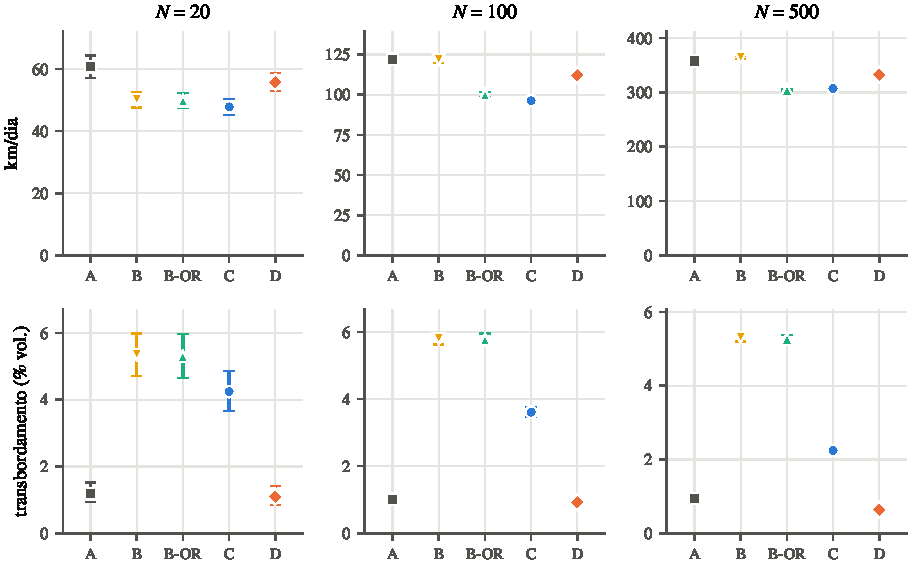
\includegraphics[width=\textwidth]{figures/fig_e1.pdf}
  \caption{E1 -- distância diária e transbordamento por política e escala (média e IC 95\%, 30 sementes).}
  \label{fig:e1}
\end{figure}

\paragraph{Quando coletar (QP1).}
Com os dados de nível, as políticas B e C coletam contêineres mais cheios:
em $N = 100$, a ocupação verdadeira média na coleta foi de \FillNCemB\% (B) e
\FillNCemC\% (C), contra \FillNCemA\% na coleta periódica, e as coletas com
ocupação abaixo de 50\% caíram de \BelowNCemA\% (A) para \BelowNCemB\% (B) e
\BelowNCemC\% (C). A distribuição completa (Figura~\ref{fig:hist}) mostra que A
espalha as coletas por toda a faixa de ocupação, enquanto B as concentra
acima de 75\%. A política preditiva ocupa uma posição intermediária
(\FillNCemD\% de ocupação média; \BelowNCemD\% de coletas abaixo de 50\%):
ela antecipa visitas a contêineres que provavelmente transbordariam antes da
próxima oportunidade e, ao fazê-lo, aceita coletá-los mais vazios. Coletar
mais cheio, portanto, não é sinônimo de coletar melhor: as políticas que mais
elevam a ocupação na coleta são também as que mais deixam contêineres
transbordar.

\begin{figure}[ht]
  \centering
  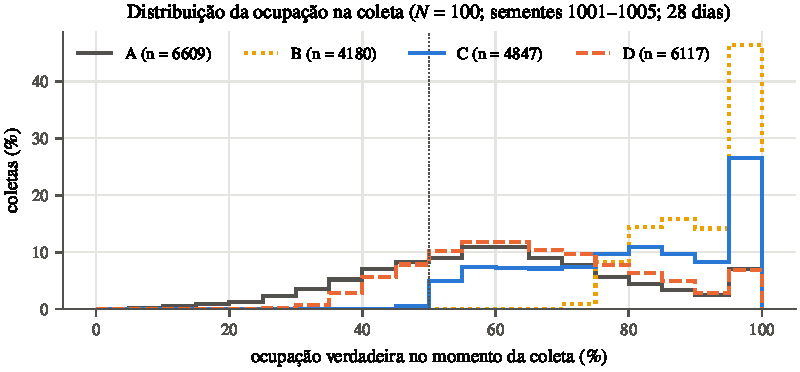
\includegraphics[width=\textwidth]{figures/fig_hist_coleta.pdf}
  \caption{Distribuição da ocupação verdadeira no momento da coleta ($N=100$; cinco sementes; 28 dias avaliados).}
  \label{fig:hist}
\end{figure}

\paragraph{Diferenças operacionais (QP2).}
Os resultados confirmam parcialmente as hipóteses pré-especificadas.
\emph{H2a} se confirma: C percorreu menos que A em todas as escalas, com
redução de \RelNVinteCvsAKm\%, \RelNCemCvsAKm\% e \RelNQuinhentosCvsAKm\% para
20, 100 e 500 contêineres ($p_{\mathrm{Holm}}$ \PNCemCvsAKm{} em $N = 100$;
$r_{rb} = -1$, isto é, menor distância em todas as 30 sementes). Mas essa
economia veio acompanhada de transbordamento maior: \OvNCemC\% do volume
gerado em C contra \OvNCemA\% em A ($N = 100$), uma diferença de
\DifNCemCvsAOv{} pontos percentuais (IC 95\%: \LoNCemCvsAOv{} a
\HiNCemCvsAOv). \emph{H2b} se confirma com folga: B transbordou
\OvNCemB\% do volume em $N = 100$, cerca de quatro vezes o valor de A, e só
visita contêineres que já estão perto do limite. O roteirizador também pesa:
com o vizinho mais próximo e 2-opt, B percorreu \RelNCemBvsAKm\% e
\RelNQuinhentosBvsAKm\% a mais que A em $N = 100$ e $N = 500$; com o OR-Tools
(B-OR), a mesma seleção percorreu \RelNCemBORvsAKm\% e
\RelNQuinhentosBORvsAKm\% em relação a A. Isso mostra que parte do ganho
atribuído à ``coleta inteligente'' em comparações informais pode vir apenas da
qualidade do roteirizador.

\emph{H2c} também se confirma: D transbordou menos que C em todas as escalas
(\OvNCemD\% contra \OvNCemC\% em $N = 100$; $p_{\mathrm{Holm}}$
\PNCemDvsCOv) e percorreu mais (\RelNCemDvsCKm\%). O resultado mais
relevante para a questão prática, porém, é a comparação com a linha de base:
D percorreu \RelNCemDvsAKm\% e \RelNQuinhentosDvsAKm\% em relação a A, em
$N = 100$ e $N = 500$, e ao mesmo tempo transbordou menos
(\RelNCemDvsAOv\% e \RelNQuinhentosDvsAOv\%; $p_{\mathrm{Holm}}$
\PNCemDvsAOv{} e \PNQuinhentosDvsAOv). Em $N = 20$, a redução de distância de
D (\RelNVinteDvsAKm\%) foi significativa, mas a de transbordamento
(\RelNVinteDvsAOv\%) não foi ($p_{\mathrm{Holm}} = $~\PNVinteDvsAOv). Com
poucos contêineres espalhados pela cidade, cada visita exige deslocamentos
longos, e a escolha de quais pontos visitar tem pouco efeito sobre a
distância total.

\begin{table}[ht]
\centering
\caption{E1 -- comparações pareadas de km/dia (alternativa $-$ referência; 30 pares; $r_{rb}$: correlação bisserial de postos; $p$ ajustado por Holm na família E1/km).}
\label{tab:e1km}
\scriptsize
\resizebox{\textwidth}{!}{\begin{tabular}{@{}llrcrrr@{}}
\toprule
Escala & Comparação & Dif. média & IC 95\% & Dif. (\%) & $r_{rb}$ & $p$ (Holm) \\
\midrule
$N=20$ & \polB{} $-$ \polA{} & $-$9,40 & [$-$10,80; $-$8,11] & $-$15,8 & $-$1,00 & $<$0,001 \\
$N=20$ & \polBOR{} $-$ \polA{} & $-$9,74 & [$-$11,20; $-$8,35] & $-$16,4 & $-$1,00 & $<$0,001 \\
$N=20$ & \polC{} $-$ \polA{} & $-$11,72 & [$-$13,11; $-$10,33] & $-$19,7 & $-$1,00 & $<$0,001 \\
$N=20$ & \polD{} $-$ \polA{} & $-$3,71 & [$-$4,70; $-$2,73] & $-$6,2 & $-$0,91 & $<$0,001 \\
$N=20$ & \polD{} $-$ \polC{} & 8,01 & [7,17; 8,84] & 16,8 & 1,00 & $<$0,001 \\
$N=20$ & \polC{} $-$ \polBOR{} & $-$1,98 & [$-$2,53; $-$1,44] & $-$4,0 & $-$0,94 & $<$0,001 \\
$N=20$ & \polBOR{} $-$ \polB{} & $-$0,33 & [$-$0,58; $-$0,11] & $-$0,7 & $-$0,57 & 0,014 \\
$N=100$ & \polB{} $-$ \polA{} & 1,75 & [0,17; 3,34] & 1,5 & 0,49 & 0,017 \\
$N=100$ & \polBOR{} $-$ \polA{} & $-$19,94 & [$-$20,91; $-$18,99] & $-$16,6 & $-$1,00 & $<$0,001 \\
$N=100$ & \polC{} $-$ \polA{} & $-$23,78 & [$-$24,77; $-$22,86] & $-$19,8 & $-$1,00 & $<$0,001 \\
$N=100$ & \polD{} $-$ \polA{} & $-$7,76 & [$-$8,60; $-$6,94] & $-$6,5 & $-$1,00 & $<$0,001 \\
$N=100$ & \polD{} $-$ \polC{} & 16,01 & [15,26; 16,73] & 16,6 & 1,00 & $<$0,001 \\
$N=100$ & \polC{} $-$ \polBOR{} & $-$3,84 & [$-$4,71; $-$3,03] & $-$3,8 & $-$1,00 & $<$0,001 \\
$N=100$ & \polBOR{} $-$ \polB{} & $-$21,70 & [$-$22,88; $-$20,58] & $-$17,8 & $-$1,00 & $<$0,001 \\
$N=500$ & \polB{} $-$ \polA{} & 13,84 & [11,33; 16,48] & 3,9 & 1,00 & $<$0,001 \\
$N=500$ & \polBOR{} $-$ \polA{} & $-$46,56 & [$-$48,14; $-$45,01] & $-$13,3 & $-$1,00 & $<$0,001 \\
$N=500$ & \polC{} $-$ \polA{} & $-$43,61 & [$-$44,97; $-$42,29] & $-$12,4 & $-$1,00 & $<$0,001 \\
$N=500$ & \polD{} $-$ \polA{} & $-$18,49 & [$-$19,91; $-$17,02] & $-$5,3 & $-$1,00 & $<$0,001 \\
$N=500$ & \polD{} $-$ \polC{} & 25,12 & [23,43; 26,76] & 8,2 & 1,00 & $<$0,001 \\
$N=500$ & \polC{} $-$ \polBOR{} & 2,95 & [1,20; 4,76] & 1,0 & 0,58 & 0,013 \\
$N=500$ & \polBOR{} $-$ \polB{} & $-$60,40 & [$-$63,16; $-$57,69] & $-$16,6 & $-$1,00 & $<$0,001 \\
\bottomrule
\end{tabular}
}
\end{table}

\begin{table}[ht]
\centering
\caption{E1 -- comparações pareadas de transbordamento (pontos percentuais do volume gerado; mesma estrutura da Tabela~\ref{tab:e1km}).}
\label{tab:e1ov}
\scriptsize
\resizebox{\textwidth}{!}{\begin{tabular}{@{}llrcrrr@{}}
\toprule
Escala & Comparação & Dif. média & IC 95\% & Dif. (\%) & $r_{rb}$ & $p$ (Holm) \\
\midrule
$N=20$ & \polB{} $-$ \polA{} & 3,98 & [3,44; 4,55] & 289,6 & 1,00 & $<$0,001 \\
$N=20$ & \polBOR{} $-$ \polA{} & 3,93 & [3,38; 4,56] & 286,6 & 1,00 & $<$0,001 \\
$N=20$ & \polC{} $-$ \polA{} & 2,87 & [2,38; 3,44] & 209,0 & 1,00 & $<$0,001 \\
$N=20$ & \polD{} $-$ \polA{} & $-$0,28 & [$-$0,49; $-$0,07] & $-$20,1 & $-$0,49 & 0,070 \\
$N=20$ & \polD{} $-$ \polC{} & $-$3,15 & [$-$3,66; $-$2,67] & $-$74,2 & $-$1,00 & $<$0,001 \\
$N=20$ & \polC{} $-$ \polBOR{} & $-$1,06 & [$-$1,32; $-$0,82] & $-$20,1 & $-$0,97 & $<$0,001 \\
$N=20$ & \polBOR{} $-$ \polB{} & $-$0,04 & [$-$0,12; 0,03] & $-$0,8 & $-$0,19 & 0,762 \\
$N=100$ & \polB{} $-$ \polA{} & 4,51 & [4,35; 4,66] & 353,7 & 1,00 & $<$0,001 \\
$N=100$ & \polBOR{} $-$ \polA{} & 4,49 & [4,32; 4,66] & 352,4 & 1,00 & $<$0,001 \\
$N=100$ & \polC{} $-$ \polA{} & 2,34 & [2,20; 2,47] & 183,2 & 1,00 & $<$0,001 \\
$N=100$ & \polD{} $-$ \polA{} & $-$0,35 & [$-$0,43; $-$0,26] & $-$27,5 & $-$0,95 & $<$0,001 \\
$N=100$ & \polD{} $-$ \polC{} & $-$2,69 & [$-$2,80; $-$2,58] & $-$74,4 & $-$1,00 & $<$0,001 \\
$N=100$ & \polC{} $-$ \polBOR{} & $-$2,16 & [$-$2,28; $-$2,04] & $-$37,4 & $-$1,00 & $<$0,001 \\
$N=100$ & \polBOR{} $-$ \polB{} & $-$0,02 & [$-$0,09; 0,06] & $-$0,3 & $-$0,09 & 0,762 \\
$N=500$ & \polB{} $-$ \polA{} & 4,11 & [4,00; 4,22] & 343,7 & 1,00 & $<$0,001 \\
$N=500$ & \polBOR{} $-$ \polA{} & 4,07 & [3,96; 4,18] & 340,3 & 1,00 & $<$0,001 \\
$N=500$ & \polC{} $-$ \polA{} & 1,04 & [0,98; 1,11] & 87,2 & 1,00 & $<$0,001 \\
$N=500$ & \polD{} $-$ \polA{} & $-$0,56 & [$-$0,60; $-$0,52] & $-$47,1 & $-$1,00 & $<$0,001 \\
$N=500$ & \polD{} $-$ \polC{} & $-$1,61 & [$-$1,65; $-$1,56] & $-$71,8 & $-$1,00 & $<$0,001 \\
$N=500$ & \polC{} $-$ \polBOR{} & $-$3,03 & [$-$3,09; $-$2,96] & $-$57,5 & $-$1,00 & $<$0,001 \\
$N=500$ & \polBOR{} $-$ \polB{} & $-$0,04 & [$-$0,08; 0,00] & $-$0,8 & $-$0,34 & 0,315 \\
\bottomrule
\end{tabular}
}
\end{table}

\subsection{Mesmo nível de serviço: fronteiras distância $\times$ transbordamento (E2)}\label{sec:e2}

As comparações do E1 dependem dos parâmetros padrão de cada política: um
limiar de 75\% em C é uma escolha, e não uma propriedade da política. O E2
varia esses parâmetros e traça, para cada política, a curva de distância
necessária para cada nível de transbordamento (Figura~\ref{fig:e2}).

\begin{figure}[ht]
  \centering
  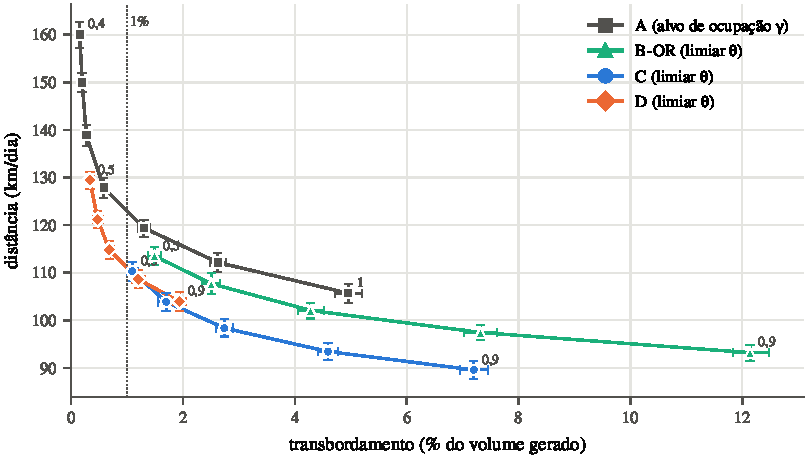
\includegraphics[width=\textwidth]{figures/fig_e2.pdf}
  \caption{E2 -- fronteiras distância $\times$ transbordamento ($N = 100$; 20 sementes por ponto; barras: IC 95\% nos dois eixos). Números junto aos pontos extremos: valor do parâmetro (ocupação-alvo $\gamma$ para A; limiar $\theta_{hi}$ para B-OR, C e D).}
  \label{fig:e2}
\end{figure}

A curva de A fica acima das demais em toda a faixa em que há sobreposição:
para manter o transbordamento em 1\% do volume gerado, A precisou, em média,
de \KmAtUmA{}~km/dia, contra \KmAtUmD{}~km/dia em D, uma redução de
\RelFrontUmDvsA\% (\NFrontUmDvsA{} sementes; $p_{\mathrm{Holm}}$
\PFrontUmDvsA). Com 2\% de transbordamento, a redução foi de
\RelFrontDoisCvsA\% para C e de \RelFrontDoisBORvsA\% para B-OR
(Tabela~\ref{tab:e2}). Onde as curvas de C e D se sobrepõem, elas ficam
próximas: com 2\%, D exigiu \RelFrontDoisDvsC\% de distância em relação a C
(\NFrontDoisDvsC{} sementes em que ambos alcançam o nível). B-OR, que não usa
contêineres opcionais, fica entre A e C.

\begin{table}[ht]
\centering
\caption{E2 -- distância necessária no mesmo nível de transbordamento (interpolação por semente; diferença em km/dia). Comparações com menos de 20 pares correspondem a sementes em que uma das políticas não alcança o nível dentro da faixa varrida.}
\label{tab:e2}
\scriptsize
\resizebox{\textwidth}{!}{\begin{tabular}{@{}llrcrrr@{}}
\toprule
Transb. & Comparação & Dif. média & IC 95\% & Dif. (\%) & $r_{rb}$ & $p$ (Holm) \\
\midrule
1,0\% & \polBOR{} $-$ \polA{} & $-$4,12 & [$-$5,51; $-$2,78] & $-$3,3 & $-$0,97 & $<$0,001 \\
1,0\% & \polC{} $-$ \polA{} & $-$10,84 & [$-$12,78; $-$9,01] & $-$8,8 & $-$1,00 & $<$0,001 \\
1,0\% & \polD{} $-$ \polA{} & $-$11,88 & [$-$13,55; $-$10,31] & $-$9,7 & $-$1,00 & $<$0,001 \\
1,0\% & \polD{} $-$ \polC{} & $-$1,03 & [$-$2,36; 0,31] & $-$0,9 & $-$0,33 & 0,202 \\
2,0\% & \polBOR{} $-$ \polA{} & $-$4,69 & [$-$5,66; $-$3,73] & $-$4,1 & $-$1,00 & $<$0,001 \\
2,0\% & \polC{} $-$ \polA{} & $-$13,07 & [$-$14,16; $-$12,00] & $-$11,3 & $-$1,00 & $<$0,001 \\
2,0\% & \polD{} $-$ \polA{} & $-$11,21 & [$-$12,02; $-$10,43] & $-$9,7 & $-$1,00 & $<$0,001 \\
2,0\% & \polD{} $-$ \polC{} & 1,86 & [1,03; 2,71] & 1,8 & 0,86 & $<$0,001 \\
\bottomrule
\end{tabular}
}
\end{table}

Essa análise muda a leitura do E1. A diferença entre C e D no E1 não indica
que a previsão seja necessária para obter ganhos; indica sobretudo que, com os
parâmetros padrão, C opera em um ponto de mais transbordamento da fronteira e
D em um ponto de menos. A vantagem robusta, observada em ambos, é a da seleção
orientada por dados sobre o calendário fixo: para o mesmo nível de serviço,
cerca de 10\% menos distância. A previsão serve, na prática, para alcançar
níveis baixos de transbordamento (abaixo de 1\%) que C só atinge com limiares
mais baixos e mais visitas. Esse valor, \RelFrontUmDvsA\%, é menor que os
ganhos médios relatados por estudos de simulação na meta-análise de
\cite{maciel2025impact} (cerca de 40\%) e próximo da média de implantações
reais (cerca de 12\%). Uma explicação plausível é que a linha de base aqui
é exigente: A tem frequências ajustadas contêiner a contêiner, com as taxas
médias verdadeiras, e rotas otimizadas pelo mesmo resolvedor.

\paragraph{Previsão.}
O preditor de taxa usado por D teve erro absoluto médio de \PredNCemD{} (em
fração do volume) para a ocupação 24~h à frente, contra \PersistNCemD{} da
persistência, em $N = 100$. Os erros foram calculados apenas para contêineres
sem coleta no intervalo e incluem o efeito do ruído de medição.

\subsection{Robustez a falhas de telemetria (E3)}\label{sec:e3}

O E3 perturba um fator por vez no cenário-base ($N = 100$). A
Tabela~\ref{tab:e3} mostra o transbordamento médio de cada política e a
disponibilidade de telemetria, e a Figura~\ref{fig:e3} mostra as mesmas médias
com seus intervalos. A política A não usa telemetria e serve de referência
fixa. A Tabela~\ref{tab:e3deg} compara cada condição com a base, dentro de
cada política.

\begin{table}[ht]
\centering
\caption{E3 -- transbordamento médio por condição e disponibilidade de telemetria (leituras válidas entregues/leituras programadas, na política C). Última coluna: distância de D. 30 sementes por célula; $N = 100$.}
\label{tab:e3}
\scriptsize
\resizebox{\textwidth}{!}{\begin{tabular}{@{}lrrrrrr@{}}
\toprule
 & Telemetria & \multicolumn{4}{c}{Transbordamento (\% do volume)} & km/dia \\
\cmidrule(lr){3-6}
Condição & disponível (\%) & \polA{} & \polBOR{} & \polC{} & \polD{} & \polD{} \\
\midrule
base & 97,2 & 1,28 & 5,77 & 3,61 & 0,92 & 112,2 \\
perda 5\% & 93,2 & 1,28 & 5,74 & 3,64 & 0,91 & 112,3 \\
perda 20\% & 78,5 & 1,28 & 5,82 & 3,61 & 0,88 & 113,1 \\
perda 50\% & 49,1 & 1,28 & 6,02 & 3,77 & 0,83 & 114,5 \\
interrupcao 48h & 84,8 & 1,28 & 6,36 & 4,06 & 0,89 & 113,2 \\
\bottomrule
\end{tabular}
}
\end{table}

\begin{figure}[ht]
  \centering
  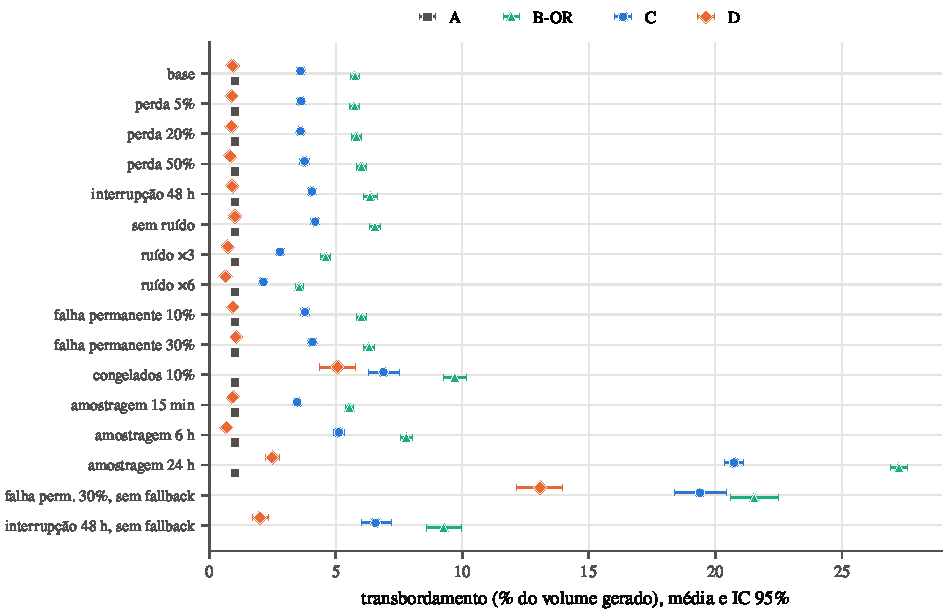
\includegraphics[width=\textwidth]{figures/fig_e3.pdf}
  \caption{E3 -- transbordamento por condição de telemetria (média e IC 95\%; 30 sementes; $N = 100$).}
  \label{fig:e3}
\end{figure}

\paragraph{Perda de mensagens e interrupções.}
Perdas independentes de 5\% e 20\% das mensagens não alteraram o
transbordamento de forma detectável em nenhuma política. Mesmo com 50\% de
perda, quando só metade das leituras chegou à plataforma, o efeito foi pequeno:
\DifETdegradacaoPerdaCZBORvsBOROv{} p.p. em B-OR ($p_{\mathrm{Holm}} =$
\PETdegradacaoPerdaCZBORvsBOROv), \DifETdegradacaoPerdaCZCvsCOv{} p.p. em C
(não significativo) e \DifETdegradacaoPerdaCZDvsDOv{} p.p. em D. Com uma
leitura por hora e decisões uma vez por dia, a plataforma tolera muitas
lacunas: basta que alguma leitura recente chegue antes do planejamento. As
interrupções regionais de 48~h, que deixam metade dos dispositivos sem
comunicação, tiveram efeito maior em B-OR
(+\DifETdegradacaoInterrupcaoQOHBORvsBOROv{} p.p.) e em C
(+\DifETdegradacaoInterrupcaoQOHCvsCOv{} p.p.; ambos $p_{\mathrm{Holm}}$
\PETdegradacaoInterrupcaoQOHCvsCOv), mas não em D
(\DifETdegradacaoInterrupcaoQOHDvsDOv{} p.p.; $p_{\mathrm{Holm}} =$
\PETdegradacaoInterrupcaoQOHDvsDOv).

\paragraph{Estimativa para dados desatualizados (H3b).}
O mecanismo de \emph{fallback}, que projeta a ocupação dos contêineres sem
dado recente pela taxa de longo prazo, foi decisivo. Com 30\% dos sensores em
falha permanente e o \emph{fallback} ativo, o transbordamento de C aumentou
\DifETdegradacaoFalhaPermTZCvsCOv{} p.p. em relação à base. Sem ele, isto é,
mantendo indefinidamente o último valor lido, o aumento foi de
\DifETdegradacaoFalhaPermTZSemFallbackCvsCOv{} p.p.; em D, de
\DifETdegradacaoFalhaPermTZDvsDOv{} p.p. com \emph{fallback} e
\DifETdegradacaoFalhaPermTZSemFallbackDvsDOv{} p.p. sem ele. Nas interrupções
de 48~h, desligar o \emph{fallback} elevou o aumento de C de
\DifETdegradacaoInterrupcaoQOHCvsCOv{} para
\DifETdegradacaoInterrupcaoQOHSemFallbackCvsCOv{} p.p. A hipótese H3b se
confirma. Um contêiner que para de reportar continua a encher, e uma
plataforma que trata o último valor lido como atual deixa de visitá-lo.

\paragraph{Falhas que a plataforma não detecta.}
Os sensores congelados (10\% dos dispositivos passam a repetir sempre a mesma
leitura, a partir de um instante sorteado) foram a perturbação mais grave
entre as de menor intensidade: +\DifETdegradacaoCongeladoUZBORvsBOROv{} p.p.
em B-OR, +\DifETdegradacaoCongeladoUZCvsCOv{} p.p. em C e
+\DifETdegradacaoCongeladoUZDvsDOv{} p.p. em D. O transbordamento de D
passou de valores próximos aos de A para cerca de cinco vezes o de A. Ao
contrário do sensor que se cala, o sensor congelado continua a enviar
mensagens válidas e recentes. O critério de desatualização não o identifica,
e o \emph{fallback} não é acionado. A ingestão implementada não verifica se
a ocupação permanece constante por tempo anormal. Essa verificação é simples
e deve preceder qualquer uso operacional (Seção~\ref{sec:limitacoes}).

\paragraph{Ruído e período de amostragem.}
O resultado contrário à hipótese H3a veio do ruído. Eliminar todo o erro de
medição \emph{aumentou} o transbordamento de B-OR, C e D
(+\DifETdegradacaoRuidoZBORvsBOROv, +\DifETdegradacaoRuidoZCvsCOv{} e
+\DifETdegradacaoRuidoZDvsDOv{} p.p.), e triplicar ou sextuplicar o ruído o
\emph{reduziu} (em C, \DifETdegradacaoRuidoTXCvsCOv{} e
\DifETdegradacaoRuidoSXCvsCOv{} p.p.), ao custo de mais distância
(Tabela~\ref{tab:e3}). O motivo está no modelo de medição
(Seção~\ref{sec:metodologia}). O termo de superfície irregular sempre encurta
a distância medida, porque o pulso reflete no pico da pilha. Por isso, ele
desloca a ocupação observada para cima, em média cerca de 0,8 vez o seu
desvio-padrão. Nas condições do E3, esse viés foi escalado junto com o ruído
simétrico e funcionou como margem de segurança: o contêiner parece mais cheio
do que está e é visitado antes. O E3, portanto, não separa o efeito do ruído
simétrico do efeito do viés sistemático, o que fica como limitação do
desenho. Em termos práticos, um limiar de 75\% sobre leituras enviesadas
para cima equivale a um limiar menor sobre a ocupação verdadeira, e a
calibração do sensor em campo altera o ponto de operação das políticas.

O período de amostragem separou as políticas. Com uma leitura a cada 6~h, o
transbordamento de C aumentou \DifETdegradacaoAmostraSHCvsCOv{} p.p.; com uma
a cada 24~h, \DifETdegradacaoAmostraDQHCvsCOv{} p.p., e o de B-OR,
\DifETdegradacaoAmostraDQHBORvsBOROv{} p.p. Em D, o aumento foi de
\DifETdegradacaoAmostraDQHDvsDOv{} p.p. com amostragem diária, e com 6~h o
transbordamento caiu (\DifETdegradacaoAmostraSHDvsDOv{} p.p.). As políticas
que decidem pelo valor observado dependem de dados frequentes, porque o valor
lido envelhece até o planejamento. A política que projeta a ocupação pela
taxa estimada compensa boa parte desse envelhecimento. Amostrar a cada 15
minutos, em vez de 1~h, não trouxe benefício relevante a nenhuma política.
Isso interessa ao projeto do dispositivo, porque cada leitura transmitida
consome energia.

\begin{table}[ht]
\centering
\caption{E3 -- variação do transbordamento em relação à base, dentro de cada política (p.p. do volume gerado; 30 pares; Holm na família E3/transbordamento).}
\label{tab:e3deg}
\scriptsize
\resizebox{\textwidth}{!}{\begin{tabular}{@{}llrcrrr@{}}
\toprule
Condição & Comparação & Dif. média & IC 95\% & Dif. (\%) & $r_{rb}$ & $p$ (Holm) \\
\midrule
perda 5\% & \polBOR{} (cond. $-$ base) & $-$0,02 & [$-$0,09; 0,04] & $-$0,4 & $-$0,11 & 1,000 \\
perda 20\% & \polBOR{} (cond. $-$ base) & 0,05 & [$-$0,02; 0,13] & 0,9 & 0,28 & 1,000 \\
perda 50\% & \polBOR{} (cond. $-$ base) & 0,25 & [0,15; 0,34] & 4,3 & 0,79 & 0,001 \\
interrupção 48 h & \polBOR{} (cond. $-$ base) & 0,59 & [0,41; 0,79] & 10,2 & 0,95 & $<$0,001 \\
sem ruído & \polBOR{} (cond. $-$ base) & 0,78 & [0,67; 0,89] & 13,6 & 1,00 & $<$0,001 \\
ruído $\times$3 & \polBOR{} (cond. $-$ base) & $-$1,16 & [$-$1,25; $-$1,07] & $-$20,1 & $-$1,00 & $<$0,001 \\
ruído $\times$6 & \polBOR{} (cond. $-$ base) & $-$2,21 & [$-$2,31; $-$2,10] & $-$38,2 & $-$1,00 & $<$0,001 \\
falha permanente 10\% & \polBOR{} (cond. $-$ base) & 0,24 & [0,14; 0,34] & 4,2 & 0,78 & 0,002 \\
falha permanente 30\% & \polBOR{} (cond. $-$ base) & 0,55 & [0,42; 0,68] & 9,5 & 0,97 & $<$0,001 \\
congelados 10\% & \polBOR{} (cond. $-$ base) & 3,94 & [3,49; 4,39] & 68,2 & 1,00 & $<$0,001 \\
amostragem 15 min & \polBOR{} (cond. $-$ base) & $-$0,23 & [$-$0,34; $-$0,11] & $-$3,9 & $-$0,71 & 0,008 \\
amostragem 6 h & \polBOR{} (cond. $-$ base) & 2,02 & [1,88; 2,15] & 35,0 & 1,00 & $<$0,001 \\
amostragem 24 h & \polBOR{} (cond. $-$ base) & 21,48 & [21,22; 21,73] & 372,4 & 1,00 & $<$0,001 \\
falha perm. 30\%, sem \emph{fallback} & \polBOR{} (cond. $-$ base) & 15,22 & [14,30; 16,18] & 240,8 & 1,00 & $<$0,001 \\
interrupção 48 h, sem \emph{fallback} & \polBOR{} (cond. $-$ base) & 2,91 & [2,37; 3,46] & 45,7 & 1,00 & $<$0,001 \\
perda 5\% & \polC{} (cond. $-$ base) & 0,03 & [$-$0,05; 0,12] & 0,8 & 0,05 & 1,000 \\
perda 20\% & \polC{} (cond. $-$ base) & 0,00 & [$-$0,08; 0,08] & $-$0,1 & $-$0,09 & 1,000 \\
perda 50\% & \polC{} (cond. $-$ base) & 0,16 & [0,04; 0,27] & 4,3 & 0,48 & 0,375 \\
interrupção 48 h & \polC{} (cond. $-$ base) & 0,45 & [0,31; 0,58] & 12,4 & 0,95 & $<$0,001 \\
sem ruído & \polC{} (cond. $-$ base) & 0,58 & [0,47; 0,70] & 16,1 & 0,99 & $<$0,001 \\
ruído $\times$3 & \polC{} (cond. $-$ base) & $-$0,81 & [$-$0,90; $-$0,72] & $-$22,5 & $-$1,00 & $<$0,001 \\
ruído $\times$6 & \polC{} (cond. $-$ base) & $-$1,47 & [$-$1,54; $-$1,39] & $-$40,7 & $-$1,00 & $<$0,001 \\
falha permanente 10\% & \polC{} (cond. $-$ base) & 0,18 & [0,07; 0,28] & 4,9 & 0,57 & 0,095 \\
falha permanente 30\% & \polC{} (cond. $-$ base) & 0,47 & [0,37; 0,57] & 13,0 & 0,99 & $<$0,001 \\
congelados 10\% & \polC{} (cond. $-$ base) & 3,28 & [2,69; 3,91] & 90,7 & 1,00 & $<$0,001 \\
amostragem 15 min & \polC{} (cond. $-$ base) & $-$0,13 & [$-$0,24; $-$0,02] & $-$3,6 & $-$0,45 & 0,469 \\
amostragem 6 h & \polC{} (cond. $-$ base) & 1,51 & [1,38; 1,64] & 41,9 & 1,00 & $<$0,001 \\
amostragem 24 h & \polC{} (cond. $-$ base) & 17,13 & [16,81; 17,43] & 474,5 & 1,00 & $<$0,001 \\
falha perm. 30\%, sem \emph{fallback} & \polC{} (cond. $-$ base) & 15,31 & [14,36; 16,30] & 375,3 & 1,00 & $<$0,001 \\
interrupção 48 h, sem \emph{fallback} & \polC{} (cond. $-$ base) & 2,51 & [2,02; 3,05] & 62,0 & 1,00 & $<$0,001 \\
perda 5\% & \polD{} (cond. $-$ base) & $-$0,02 & [$-$0,06; 0,03] & $-$1,8 & $-$0,10 & 1,000 \\
perda 20\% & \polD{} (cond. $-$ base) & $-$0,04 & [$-$0,09; 0,01] & $-$4,5 & $-$0,30 & 1,000 \\
perda 50\% & \polD{} (cond. $-$ base) & $-$0,09 & [$-$0,14; $-$0,04] & $-$9,7 & $-$0,66 & 0,024 \\
interrupção 48 h & \polD{} (cond. $-$ base) & $-$0,01 & [$-$0,06; 0,03] & $-$1,6 & $-$0,13 & 1,000 \\
sem ruído & \polD{} (cond. $-$ base) & 0,10 & [0,05; 0,14] & 10,3 & 0,70 & 0,010 \\
ruído $\times$3 & \polD{} (cond. $-$ base) & $-$0,18 & [$-$0,22; $-$0,14] & $-$19,7 & $-$0,96 & $<$0,001 \\
ruído $\times$6 & \polD{} (cond. $-$ base) & $-$0,28 & [$-$0,33; $-$0,23] & $-$30,1 & $-$0,99 & $<$0,001 \\
falha permanente 10\% & \polD{} (cond. $-$ base) & 0,02 & [$-$0,02; 0,06] & 2,3 & 0,14 & 1,000 \\
falha permanente 30\% & \polD{} (cond. $-$ base) & 0,13 & [0,07; 0,19] & 13,6 & 0,77 & 0,002 \\
congelados 10\% & \polD{} (cond. $-$ base) & 4,15 & [3,46; 4,88] & 448,7 & 1,00 & $<$0,001 \\
amostragem 15 min & \polD{} (cond. $-$ base) & 0,01 & [$-$0,04; 0,06] & 0,9 & 0,06 & 1,000 \\
amostragem 6 h & \polD{} (cond. $-$ base) & $-$0,24 & [$-$0,28; $-$0,19] & $-$25,5 & $-$1,00 & $<$0,001 \\
amostragem 24 h & \polD{} (cond. $-$ base) & 1,57 & [1,32; 1,84] & 169,5 & 1,00 & $<$0,001 \\
falha perm. 30\%, sem \emph{fallback} & \polD{} (cond. $-$ base) & 12,03 & [11,10; 12,90] & 1.145,3 & 1,00 & $<$0,001 \\
interrupção 48 h, sem \emph{fallback} & \polD{} (cond. $-$ base) & 1,10 & [0,82; 1,40] & 120,6 & 1,00 & $<$0,001 \\
\bottomrule
\end{tabular}
}
\end{table}

\subsection{Sensibilidade operacional (E4)}\label{sec:e4}

O E4 varia a demanda, a frota, o arranjo espacial e a velocidade. A
Figura~\ref{fig:e4} mostra, para cada condição, a diferença pareada de cada
política em relação a A, e as Tabelas~\ref{tab:e4km} e~\ref{tab:e4ov} trazem
os valores.

\begin{figure}[ht]
  \centering
  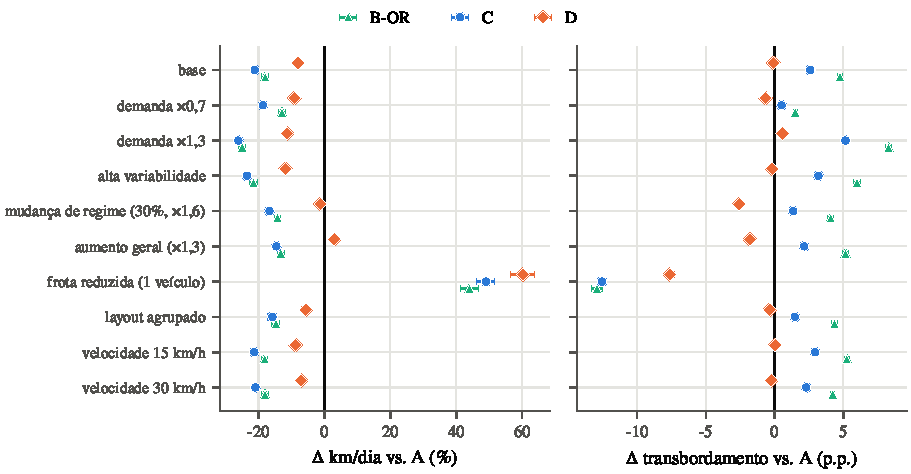
\includegraphics[width=\textwidth]{figures/fig_e4.pdf}
  \caption{E4 -- diferença pareada em relação a A por condição (média e IC 95\%; 30 sementes; $N = 100$). Esquerda: distância (\% de A); direita: transbordamento (pontos percentuais).}
  \label{fig:e4}
\end{figure}

\paragraph{Mudança na demanda (H4).}
A política A planeja o calendário com a taxa média verdadeira de cada
contêiner, mas não acompanha mudanças posteriores. Quando 30\% dos
contêineres passam a gerar 60\% a mais a partir do 14.º dia, o
transbordamento médio de A sobe de \OvNCemA\% para cerca de 4\%. O de D
sobe menos e fica \DifEQMudancaRegimeTZXUSDvsAOv{} p.p. em relação a A
($p_{\mathrm{Holm}}$ \PEQMudancaRegimeTZXUSDvsAOv), com distância
praticamente igual (\RelEQMudancaRegimeTZXUSDvsAKm\%). O mesmo padrão aparece
no aumento geral de 30\% da demanda (\DifEQSurtoGeralXUTDvsAOv{} p.p.), agora
com \RelEQSurtoGeralXUTDvsAKm\% de distância. C também se degrada menos que
A nessas condições, mas parte de um transbordamento maior e continua acima
dela. A hipótese H4 se confirma para mudanças de regime. É nelas que o
componente preditivo mostra seu valor mais claro. Quando a intensidade muda
desde o início e A a conhece (demanda $\times 0{,}7$ e $\times 1{,}3$), A
mantém cerca de 1\% de transbordamento. Ainda assim, com demanda baixa, D
reduziu ao mesmo tempo a distância (\RelEQDemandaZSeDvsAKm\%) e o
transbordamento (\DifEQDemandaZSeDvsAOv{} p.p.), e as reduções de distância
de C cresceram com a intensidade (\RelEQDemandaZSeCvsAKm\%,
\RelEQBaseCvsAKm\% e \RelEQDemandaUTCvsAKm\% para $\times 0{,}7$, base e
$\times 1{,}3$).

\paragraph{Frota insuficiente.}
Com um único veículo, a capacidade planejada (uma viagem de
26.000~L por turno, pela regra de execução do modelo) fica abaixo do
volume gerado por dia, e nenhuma política evita o transbordamento: A chegou a
31\%, e as demais ficaram entre 18\% e 24\% (Tabela~\ref{tab:e4ov}). Nessa
escassez, as políticas com telemetria transbordaram
\DifEQFrotaReduzidaCvsAOv{} p.p. (C) e \DifEQFrotaReduzidaDvsAOv{} p.p. (D)
em relação a A, porque priorizam os contêineres mais cheios. Em
contrapartida, percorreram mais (\RelEQFrotaReduzidaCvsAKm\% e
\RelEQFrotaReduzidaDvsAKm\%). Esse
resultado não indica que a telemetria substitua frota. Indica que, quando a
frota é insuficiente, os dados ajudam a decidir quem fica sem coleta.

\paragraph{Arranjo espacial e velocidade.}
Com contêineres agrupados em poucas áreas, todas as distâncias caem e D
reduziu a distância (\RelEQLayoutAgrupadoDvsAKm\%) e o transbordamento
(\DifEQLayoutAgrupadoDvsAOv{} p.p.) em relação a A. A velocidade do veículo
(15 ou 30~km/h) praticamente não alterou as diferenças relativas. No
cenário-base, a jornada de 8~h tem folga: em A, cada um dos dois veículos se
desloca cerca de 3~h por dia a 20~km/h.

\begin{table}[ht]
\centering
\caption{E4 -- comparações pareadas de km/dia por condição (alternativa $-$ referência; 30 pares; Holm na família E4/km).}
\label{tab:e4km}
\scriptsize
\resizebox{\textwidth}{!}{\begin{tabular}{@{}llrcrrr@{}}
\toprule
Condição & Comparação & Dif. média & IC 95\% & Dif. (\%) & $r_{rb}$ & $p$ (Holm) \\
\midrule
base & \polBOR{} $-$ \polA{} & $-$21,98 & [$-$23,19; $-$20,71] & $-$18,0 & $-$1,00 & $<$0,001 \\
base & \polC{} $-$ \polA{} & $-$25,81 & [$-$26,95; $-$24,61] & $-$21,2 & $-$1,00 & $<$0,001 \\
base & \polD{} $-$ \polA{} & $-$9,80 & [$-$10,97; $-$8,51] & $-$8,0 & $-$1,00 & $<$0,001 \\
base & \polD{} $-$ \polC{} & 16,01 & [15,28; 16,75] & 16,6 & 1,00 & $<$0,001 \\
demanda $\times$0,7 & \polBOR{} $-$ \polA{} & $-$12,69 & [$-$13,72; $-$11,66] & $-$12,9 & $-$1,00 & $<$0,001 \\
demanda $\times$0,7 & \polC{} $-$ \polA{} & $-$18,43 & [$-$19,49; $-$17,36] & $-$18,7 & $-$1,00 & $<$0,001 \\
demanda $\times$0,7 & \polD{} $-$ \polA{} & $-$8,98 & [$-$9,89; $-$8,03] & $-$9,1 & $-$1,00 & $<$0,001 \\
demanda $\times$0,7 & \polD{} $-$ \polC{} & 9,45 & [8,58; 10,24] & 11,8 & 1,00 & $<$0,001 \\
demanda $\times$1,3 & \polBOR{} $-$ \polA{} & $-$36,94 & [$-$38,49; $-$35,36] & $-$25,0 & $-$1,00 & $<$0,001 \\
demanda $\times$1,3 & \polC{} $-$ \polA{} & $-$38,63 & [$-$40,14; $-$37,10] & $-$26,1 & $-$1,00 & $<$0,001 \\
demanda $\times$1,3 & \polD{} $-$ \polA{} & $-$16,75 & [$-$18,07; $-$15,40] & $-$11,3 & $-$1,00 & $<$0,001 \\
demanda $\times$1,3 & \polD{} $-$ \polC{} & 21,89 & [21,09; 22,68] & 20,0 & 1,00 & $<$0,001 \\
alta variabilidade & \polBOR{} $-$ \polA{} & $-$27,56 & [$-$28,99; $-$26,11] & $-$21,5 & $-$1,00 & $<$0,001 \\
alta variabilidade & \polC{} $-$ \polA{} & $-$30,07 & [$-$31,46; $-$28,67] & $-$23,5 & $-$1,00 & $<$0,001 \\
alta variabilidade & \polD{} $-$ \polA{} & $-$15,08 & [$-$16,33; $-$13,94] & $-$11,8 & $-$1,00 & $<$0,001 \\
alta variabilidade & \polD{} $-$ \polC{} & 14,99 & [14,33; 15,64] & 15,3 & 1,00 & $<$0,001 \\
mudança de regime (30\%, $\times$1,6) & \polBOR{} $-$ \polA{} & $-$17,40 & [$-$18,65; $-$16,16] & $-$14,2 & $-$1,00 & $<$0,001 \\
mudança de regime (30\%, $\times$1,6) & \polC{} $-$ \polA{} & $-$20,38 & [$-$21,56; $-$19,18] & $-$16,7 & $-$1,00 & $<$0,001 \\
mudança de regime (30\%, $\times$1,6) & \polD{} $-$ \polA{} & $-$1,57 & [$-$2,82; $-$0,24] & $-$1,3 & $-$0,55 & 0,008 \\
mudança de regime (30\%, $\times$1,6) & \polD{} $-$ \polC{} & 18,82 & [18,07; 19,56] & 18,5 & 1,00 & $<$0,001 \\
aumento geral ($\times$1,3) & \polBOR{} $-$ \polA{} & $-$16,48 & [$-$17,87; $-$14,99] & $-$13,2 & $-$1,00 & $<$0,001 \\
aumento geral ($\times$1,3) & \polC{} $-$ \polA{} & $-$18,14 & [$-$19,38; $-$16,77] & $-$14,6 & $-$1,00 & $<$0,001 \\
aumento geral ($\times$1,3) & \polD{} $-$ \polA{} & 3,74 & [2,46; 5,25] & 3,0 & 0,94 & $<$0,001 \\
aumento geral ($\times$1,3) & \polD{} $-$ \polC{} & 21,88 & [21,05; 22,73] & 20,6 & 1,00 & $<$0,001 \\
frota reduzida (1 veículo) & \polBOR{} $-$ \polA{} & 23,60 & [22,19; 25,10] & 44,0 & 1,00 & $<$0,001 \\
frota reduzida (1 veículo) & \polC{} $-$ \polA{} & 26,30 & [24,81; 27,73] & 49,0 & 1,00 & $<$0,001 \\
frota reduzida (1 veículo) & \polD{} $-$ \polA{} & 32,29 & [30,24; 34,19] & 60,2 & 1,00 & $<$0,001 \\
frota reduzida (1 veículo) & \polD{} $-$ \polC{} & 5,99 & [4,36; 7,68] & 7,5 & 0,98 & $<$0,001 \\
layout agrupado & \polBOR{} $-$ \polA{} & $-$13,25 & [$-$14,53; $-$12,20] & $-$14,7 & $-$1,00 & $<$0,001 \\
layout agrupado & \polC{} $-$ \polA{} & $-$14,25 & [$-$15,49; $-$13,11] & $-$15,8 & $-$1,00 & $<$0,001 \\
layout agrupado & \polD{} $-$ \polA{} & $-$5,11 & [$-$6,25; $-$4,17] & $-$5,7 & $-$1,00 & $<$0,001 \\
layout agrupado & \polD{} $-$ \polC{} & 9,14 & [8,33; 9,95] & 12,0 & 1,00 & $<$0,001 \\
velocidade 15 km/h & \polBOR{} $-$ \polA{} & $-$22,12 & [$-$23,32; $-$20,89] & $-$18,2 & $-$1,00 & $<$0,001 \\
velocidade 15 km/h & \polC{} $-$ \polA{} & $-$25,93 & [$-$27,17; $-$24,72] & $-$21,3 & $-$1,00 & $<$0,001 \\
velocidade 15 km/h & \polD{} $-$ \polA{} & $-$10,68 & [$-$11,83; $-$9,48] & $-$8,8 & $-$1,00 & $<$0,001 \\
velocidade 15 km/h & \polD{} $-$ \polC{} & 15,25 & [14,69; 15,82] & 15,9 & 1,00 & $<$0,001 \\
velocidade 30 km/h & \polBOR{} $-$ \polA{} & $-$22,06 & [$-$23,26; $-$20,88] & $-$18,0 & $-$1,00 & $<$0,001 \\
velocidade 30 km/h & \polC{} $-$ \polA{} & $-$25,61 & [$-$26,88; $-$24,38] & $-$20,9 & $-$1,00 & $<$0,001 \\
velocidade 30 km/h & \polD{} $-$ \polA{} & $-$8,61 & [$-$9,71; $-$7,39] & $-$7,0 & $-$1,00 & $<$0,001 \\
velocidade 30 km/h & \polD{} $-$ \polC{} & 17,00 & [16,29; 17,68] & 17,6 & 1,00 & $<$0,001 \\
\bottomrule
\end{tabular}
}
\end{table}

\begin{table}[ht]
\centering
\caption{E4 -- comparações pareadas de transbordamento (p.p. do volume gerado; Holm na família E4/transbordamento).}
\label{tab:e4ov}
\scriptsize
\resizebox{\textwidth}{!}{\begin{tabular}{@{}llrcrrr@{}}
\toprule
Condição & Comparação & Dif. média & IC 95\% & Dif. (\%) & $r_{rb}$ & $p$ (Holm) \\
\midrule
base & \polBOR{} $-$ \polA{} & 4,76 & [4,59; 4,92] & 470,1 & 1,00 & $<$0,001 \\
base & \polC{} $-$ \polA{} & 2,60 & [2,47; 2,73] & 256,8 & 1,00 & $<$0,001 \\
base & \polD{} $-$ \polA{} & $-$0,09 & [$-$0,17; $-$0,01] & $-$8,7 & $-$0,40 & 0,115 \\
base & \polD{} $-$ \polC{} & $-$2,69 & [$-$2,80; $-$2,58] & $-$74,4 & $-$1,00 & $<$0,001 \\
demanda $\times$0,7 & \polBOR{} $-$ \polA{} & 1,50 & [1,34; 1,65] & 132,5 & 1,00 & $<$0,001 \\
demanda $\times$0,7 & \polC{} $-$ \polA{} & 0,51 & [0,35; 0,67] & 44,7 & 0,91 & $<$0,001 \\
demanda $\times$0,7 & \polD{} $-$ \polA{} & $-$0,65 & [$-$0,76; $-$0,55] & $-$57,8 & $-$1,00 & $<$0,001 \\
demanda $\times$0,7 & \polD{} $-$ \polC{} & $-$1,16 & [$-$1,28; $-$1,05] & $-$70,9 & $-$1,00 & $<$0,001 \\
demanda $\times$1,3 & \polBOR{} $-$ \polA{} & 8,30 & [8,09; 8,50] & 673,7 & 1,00 & $<$0,001 \\
demanda $\times$1,3 & \polC{} $-$ \polA{} & 5,16 & [4,97; 5,35] & 418,7 & 1,00 & $<$0,001 \\
demanda $\times$1,3 & \polD{} $-$ \polA{} & 0,58 & [0,49; 0,66] & 46,9 & 1,00 & $<$0,001 \\
demanda $\times$1,3 & \polD{} $-$ \polC{} & $-$4,58 & [$-$4,76; $-$4,40] & $-$71,7 & $-$1,00 & $<$0,001 \\
alta variabilidade & \polBOR{} $-$ \polA{} & 6,00 & [5,76; 6,24] & 151,6 & 1,00 & $<$0,001 \\
alta variabilidade & \polC{} $-$ \polA{} & 3,19 & [2,98; 3,39] & 80,7 & 1,00 & $<$0,001 \\
alta variabilidade & \polD{} $-$ \polA{} & $-$0,18 & [$-$0,32; $-$0,03] & $-$4,5 & $-$0,44 & 0,104 \\
alta variabilidade & \polD{} $-$ \polC{} & $-$3,37 & [$-$3,51; $-$3,22] & $-$47,1 & $-$1,00 & $<$0,001 \\
mudança de regime (30\%, $\times$1,6) & \polBOR{} $-$ \polA{} & 4,08 & [3,86; 4,29] & 97,0 & 1,00 & $<$0,001 \\
mudança de regime (30\%, $\times$1,6) & \polC{} $-$ \polA{} & 1,35 & [1,16; 1,54] & 32,2 & 1,00 & $<$0,001 \\
mudança de regime (30\%, $\times$1,6) & \polD{} $-$ \polA{} & $-$2,58 & [$-$2,72; $-$2,43] & $-$61,4 & $-$1,00 & $<$0,001 \\
mudança de regime (30\%, $\times$1,6) & \polD{} $-$ \polC{} & $-$3,93 & [$-$4,07; $-$3,79] & $-$70,8 & $-$1,00 & $<$0,001 \\
aumento geral ($\times$1,3) & \polBOR{} $-$ \polA{} & 5,16 & [4,94; 5,39] & 140,6 & 1,00 & $<$0,001 \\
aumento geral ($\times$1,3) & \polC{} $-$ \polA{} & 2,16 & [1,95; 2,38] & 58,7 & 1,00 & $<$0,001 \\
aumento geral ($\times$1,3) & \polD{} $-$ \polA{} & $-$1,80 & [$-$1,98; $-$1,61] & $-$48,9 & $-$1,00 & $<$0,001 \\
aumento geral ($\times$1,3) & \polD{} $-$ \polC{} & $-$3,95 & [$-$4,11; $-$3,80] & $-$67,8 & $-$1,00 & $<$0,001 \\
frota reduzida (1 veículo) & \polBOR{} $-$ \polA{} & $-$12,91 & [$-$13,28; $-$12,54] & $-$41,0 & $-$1,00 & $<$0,001 \\
frota reduzida (1 veículo) & \polC{} $-$ \polA{} & $-$12,56 & [$-$12,91; $-$12,20] & $-$39,9 & $-$1,00 & $<$0,001 \\
frota reduzida (1 veículo) & \polD{} $-$ \polA{} & $-$7,62 & [$-$7,96; $-$7,30] & $-$24,2 & $-$1,00 & $<$0,001 \\
frota reduzida (1 veículo) & \polD{} $-$ \polC{} & 4,94 & [4,77; 5,10] & 26,1 & 1,00 & $<$0,001 \\
layout agrupado & \polBOR{} $-$ \polA{} & 4,35 & [4,16; 4,55] & 437,6 & 1,00 & $<$0,001 \\
layout agrupado & \polC{} $-$ \polA{} & 1,48 & [1,36; 1,60] & 148,9 & 1,00 & $<$0,001 \\
layout agrupado & \polD{} $-$ \polA{} & $-$0,35 & [$-$0,42; $-$0,28] & $-$35,4 & $-$1,00 & $<$0,001 \\
layout agrupado & \polD{} $-$ \polC{} & $-$1,83 & [$-$1,95; $-$1,71] & $-$74,1 & $-$1,00 & $<$0,001 \\
velocidade 15 km/h & \polBOR{} $-$ \polA{} & 5,26 & [5,07; 5,46] & 497,4 & 1,00 & $<$0,001 \\
velocidade 15 km/h & \polC{} $-$ \polA{} & 2,95 & [2,80; 3,11] & 278,5 & 1,00 & $<$0,001 \\
velocidade 15 km/h & \polD{} $-$ \polA{} & 0,03 & [$-$0,06; 0,11] & 2,9 & 0,14 & 0,503 \\
velocidade 15 km/h & \polD{} $-$ \polC{} & $-$2,92 & [$-$3,06; $-$2,77] & $-$72,8 & $-$1,00 & $<$0,001 \\
velocidade 30 km/h & \polBOR{} $-$ \polA{} & 4,22 & [4,07; 4,38] & 422,8 & 1,00 & $<$0,001 \\
velocidade 30 km/h & \polC{} $-$ \polA{} & 2,30 & [2,15; 2,45] & 230,1 & 1,00 & $<$0,001 \\
velocidade 30 km/h & \polD{} $-$ \polA{} & $-$0,24 & [$-$0,31; $-$0,16] & $-$23,5 & $-$0,87 & $<$0,001 \\
velocidade 30 km/h & \polD{} $-$ \polC{} & $-$2,53 & [$-$2,66; $-$2,41] & $-$76,8 & $-$1,00 & $<$0,001 \\
\bottomrule
\end{tabular}
}
\end{table}

\subsection{Sensibilidade ao resolvedor (E5)}\label{sec:e5}

Com 500 contêineres, a descida gulosa do OR-Tools levou em média
\RefSolAT{}~s (A), \RefSolCT{}~s (C) e \RefSolDT{}~s (D) por planejamento
diário. A busca local guiada (GLS), interrompida após 5~s, encontrou rotas
mais curtas: a distância diária variou \RelSolAKm\% em A, \RelSolCKm\% em C e
\RelSolDKm\% em D ($p_{\mathrm{Holm}}$: \PSolAKm, \PSolCKm{} e \PSolDKm; 10
sementes). As diferenças são pequenas diante das diferenças entre políticas,
e a ordem se manteve com os dois resolvedores: com GLS, C percorreu
\AltSolCKm{}~km/dia, D \AltSolDKm{} e A \AltSolAKm. O transbordamento
praticamente não mudou (diferenças de \DifSolAOv, \DifSolCOv{} e
\DifSolDOv{}~p.p.). Como a melhoria do GLS foi um pouco maior em A, o uso da
descida gulosa nas rodadas principais tende a favorecer levemente as
políticas com telemetria, em menos de 1\% da distância de A. A escolha da
descida gulosa, motivada pelo determinismo, não altera as conclusões.

\subsection{Relação com a literatura}\label{sec:literatura}

As reduções de distância medidas aqui são menores que as frequentemente
relatadas por estudos de simulação. Com os parâmetros padrão, C percorreu
cerca de 21\% menos que A, mas transbordou mais. No mesmo nível de serviço, a
variação ficou entre \RelFrontUmCvsA\% e \RelFrontDoisCvsA\%. Duas escolhas de
desenho explicam boa parte da diferença. A primeira é que a linha de base usa
o mesmo resolvedor e frequências ajustadas por contêiner com taxas
verdadeiras. Muitos estudos comparam a coleta inteligente com uma rota fixa
pouco otimizada, o que mistura o efeito dos dados com o efeito da
roteirização. O E1 mostrou que essa mistura é grande: em $N = 100$ e $N = 500$, só trocar
o vizinho mais próximo pelo OR-Tools reduziu a distância de B em 17\% a 18\%. A
segunda escolha é medir o transbordamento junto com a distância. Uma política
que visita apenas contêineres acima de 75\% economiza distância, mas transfere
o custo para o serviço. \cite{brouwer2023comparison} descrevem o mesmo
compromisso entre número de coletas e número de transbordamentos. Os ganhos
modestos e a importância das hipóteses sobre a demanda também são coerentes
com a meta-análise de \cite{maciel2025impact}, em que os resultados de
implantações reais ficam bem abaixo dos de simulações.

\subsection{Implicações práticas}\label{sec:implicacoes}

Para um município que avalie sensores de nível, os resultados sugerem cinco
cuidados. Eles valem para o modelo estudado e precisam ser confirmados em
campo.
\begin{enumerate}
  \item Comparar com uma linha de base bem roteirizada. Parte do ganho da
        ``coleta inteligente'' pode ser obtida apenas com melhor roteirização
        da coleta atual.
  \item Fixar o nível de serviço antes de medir a economia. Reduções de
        distância obtidas com mais transbordamento não são ganhos de
        eficiência.
  \item Tratar dados ausentes explicitamente. A estimativa por taxa para
        contêineres sem dado recente foi a diferença entre degradação
        pequena e falha grave.
  \item Detectar sensores que continuam a reportar valores implausíveis
        (constantes, por exemplo). Esse é o modo de falha mais perigoso
        encontrado.
  \item Não superdimensionar a frequência de amostragem: uma leitura por hora
        foi suficiente, e a previsão compensou leituras ainda mais
        espaçadas.
\end{enumerate}
O valor dos dados aparece mais claramente quando a demanda muda e o calendário
fixo fica defasado, situação comum em áreas de crescimento urbano, eventos e
sazonalidade turística.

\subsection{Limitações}\label{sec:limitacoes}

Os resultados valem para o modelo e os parâmetros descritos. Os perfis de
geração, a heterogeneidade entre contêineres e os descartes volumosos são
hipóteses de cenário e não foram calibrados com medições de campo. As
posições dos contêineres e do depósito são hipotéticas, e os resultados não
descrevem o serviço real de Aracaju. O veículo percorre a malha a velocidade
constante, sem trânsito, e cada veículo faz uma rota planejada por turno, com
desvios ao depósito apenas quando a carga excede a capacidade. Por isso, o
cenário de frota reduzida mede sobretudo a restrição de capacidade. O
transbordamento é modelado como volume recusado, sem efeitos sobre os
contêineres vizinhos ou sobre o comportamento da população. O E3 não separa o
ruído simétrico do viés da superfície irregular, e os fatores do E3 e do E4
foram variados um de cada vez, sem estimar interações. O resolvedor é
heurístico, e a qualidade das rotas pode variar com o tamanho da instância
(Seção~\ref{sec:e5}). A plataforma não detecta sensores congelados. O
firmware foi compilado, mas não executado em hardware, e a integração MQTT
foi verificada com dispositivos virtuais em \emph{broker} local, não em rede
celular ou Wi-Fi urbana. Por fim, a política A recebe as taxas médias
verdadeiras, um planejador que nenhum município possui. Uma linha de base
estimada com histórico real tenderia a ser pior, e as diferenças em relação a
ela seriam maiores. Esse efeito não foi quantificado.


% provisório: 07-conclusao


\bibliographystyle{sbc}
\bibliography{referencias}

\appendix
\section{Reprodução dos experimentos}\label{ap:reproducao}

O repositório do projeto contém o código, os dados brutos e os scripts
necessários para reproduzir todos os resultados. Com Python~3.12 e Docker ou
Podman, a sequência é:

\begin{small}
\begin{verbatim}
uv venv --python 3.12 .venv && source .venv/bin/activate
uv pip install -e ".[dev]"            # versões fixadas em requirements-lock.txt
python -m pytest -q                   # testes automatizados
scripts/broker.sh start               # Mosquitto 2.0.20 em 127.0.0.1:1883
python -m experiments.run E1 E2 E3 E4 --workers 5
python -m experiments.run E5 --workers 3
python -m experiments.mqtt_integration
python -m experiments.replay && python -m experiments.analysis
python -m experiments.figures && python -m experiments.animations
python scripts/verify_reproducibility.py
scripts/build_paper.sh                # TeX Live 2026 em contêiner
\end{verbatim}
\end{small}

O executor grava uma linha por execução em \texttt{experiments/raw/E*.jsonl},
com a configuração completa, a semente e as métricas, e pula execuções já
concluídas, o que permite interromper e retomar a rodada. Os manifestos
registram o \emph{commit} do código, as versões das bibliotecas e a
plataforma.

\section{Material suplementar}\label{ap:suplementar}

As animações abaixo foram geradas a partir de execuções gravadas e estão no
diretório \texttt{animations/} do repositório, em GIF e MP4. Nenhuma delas é
ilustração conceitual: os quadros reproduzem os estados registrados.

\begin{description}
  \item[A\_enchimento] Ocupação de seis contêineres ao longo de 7 dias
  (política A, semente 1001).
  \item[B\_telemetria\_mqtt] Telemetria recebida pela plataforma pelo broker
  Mosquitto em uma execução do modo \emph{live} (80 contêineres virtuais), com
  eventos de limiar.
  \item[C\_coleta\_veiculos] Veículos executando as rotas da política D na
  malha de Aracaju.
  \item[D\_comparacao\_A\_D] Comparação sincronizada das políticas A e D com a
  mesma demanda.
  \item[E\_falha\_comunicacao] Estado verdadeiro e estado visto pela plataforma
  durante uma interrupção regional de 48~h.
\end{description}

\section{Mapa de pinos do firmware 2.0}\label{ap:pinos}

\begin{table}[ht]
\centering
\caption{Ligações do protótipo com o firmware 2.0 (DOIT ESP32 DevKit V1).}
\footnotesize
\begin{tabular}{@{}lll@{}}
\toprule
Sinal & GPIO & Observação \\
\midrule
HC-SR04 TRIG & 14 & nível alto de 3,3~V é suficiente para o disparo \\
HC-SR04 ECHO & 27 & via divisor 1~k$\Omega$ (série) / 2~k$\Omega$ (terra): $5 \times 2/3 \approx 3{,}33$~V \\
DHT11 DATA & 4 & alimentação em 3,3~V; \emph{pull-up} de 4,7--10~k$\Omega$ para 3,3~V \\
LED & 2 & LED da placa; saída \\
\bottomrule
\end{tabular}
\end{table}

\section{Declaração de uso de ferramentas de inteligência artificial}\label{ap:ia}

O desenvolvimento desta versão contou com a assistência de um modelo de
linguagem (Claude, da Anthropic) na revisão bibliográfica (busca e conferência
de metadados), na escrita e revisão do código, na execução dos experimentos e
na redação do texto. Todas as referências tiveram os metadados conferidos em
fontes oficiais (Crossref, OpenAlex ou página do editor), e o registro dessa
verificação, incluindo quais textos foram lidos integralmente e quais apenas
pelo resumo, está em \texttt{paper/references/biblioteca.csv}. Os resultados
numéricos foram produzidos pelos programas do repositório e inseridos no texto
automaticamente. A responsabilidade pelo conteúdo é dos autores, e o uso dessa
assistência deve observar as normas da instituição.


\end{document}
